% Options for packages loaded elsewhere
\PassOptionsToPackage{unicode}{hyperref}
\PassOptionsToPackage{hyphens}{url}
%
\documentclass[
  ignorenonframetext,
]{beamer}
\usepackage{pgfpages}
\setbeamertemplate{caption}[numbered]
\setbeamertemplate{caption label separator}{: }
\setbeamercolor{caption name}{fg=normal text.fg}
\beamertemplatenavigationsymbolsempty
% Prevent slide breaks in the middle of a paragraph
\widowpenalties 1 10000
\raggedbottom
\setbeamertemplate{part page}{
  \centering
  \begin{beamercolorbox}[sep=16pt,center]{part title}
    \usebeamerfont{part title}\insertpart\par
  \end{beamercolorbox}
}
\setbeamertemplate{section page}{
  \centering
  \begin{beamercolorbox}[sep=12pt,center]{part title}
    \usebeamerfont{section title}\insertsection\par
  \end{beamercolorbox}
}
\setbeamertemplate{subsection page}{
  \centering
  \begin{beamercolorbox}[sep=8pt,center]{part title}
    \usebeamerfont{subsection title}\insertsubsection\par
  \end{beamercolorbox}
}
\AtBeginPart{
  \frame{\partpage}
}
\AtBeginSection{
  \ifbibliography
  \else
    \frame{\sectionpage}
  \fi
}
\AtBeginSubsection{
  \frame{\subsectionpage}
}
\usepackage{amsmath,amssymb}
\usepackage{lmodern}
\usepackage{iftex}
\ifPDFTeX
  \usepackage[T1]{fontenc}
  \usepackage[utf8]{inputenc}
  \usepackage{textcomp} % provide euro and other symbols
\else % if luatex or xetex
  \usepackage{unicode-math}
  \defaultfontfeatures{Scale=MatchLowercase}
  \defaultfontfeatures[\rmfamily]{Ligatures=TeX,Scale=1}
\fi
% Use upquote if available, for straight quotes in verbatim environments
\IfFileExists{upquote.sty}{\usepackage{upquote}}{}
\IfFileExists{microtype.sty}{% use microtype if available
  \usepackage[]{microtype}
  \UseMicrotypeSet[protrusion]{basicmath} % disable protrusion for tt fonts
}{}
\makeatletter
\@ifundefined{KOMAClassName}{% if non-KOMA class
  \IfFileExists{parskip.sty}{%
    \usepackage{parskip}
  }{% else
    \setlength{\parindent}{0pt}
    \setlength{\parskip}{6pt plus 2pt minus 1pt}}
}{% if KOMA class
  \KOMAoptions{parskip=half}}
\makeatother
\usepackage{xcolor}
\newif\ifbibliography
\usepackage{color}
\usepackage{fancyvrb}
\newcommand{\VerbBar}{|}
\newcommand{\VERB}{\Verb[commandchars=\\\{\}]}
\DefineVerbatimEnvironment{Highlighting}{Verbatim}{commandchars=\\\{\}}
% Add ',fontsize=\small' for more characters per line
\usepackage{framed}
\definecolor{shadecolor}{RGB}{248,248,248}
\newenvironment{Shaded}{\begin{snugshade}}{\end{snugshade}}
\newcommand{\AlertTok}[1]{\textcolor[rgb]{0.94,0.16,0.16}{#1}}
\newcommand{\AnnotationTok}[1]{\textcolor[rgb]{0.56,0.35,0.01}{\textbf{\textit{#1}}}}
\newcommand{\AttributeTok}[1]{\textcolor[rgb]{0.77,0.63,0.00}{#1}}
\newcommand{\BaseNTok}[1]{\textcolor[rgb]{0.00,0.00,0.81}{#1}}
\newcommand{\BuiltInTok}[1]{#1}
\newcommand{\CharTok}[1]{\textcolor[rgb]{0.31,0.60,0.02}{#1}}
\newcommand{\CommentTok}[1]{\textcolor[rgb]{0.56,0.35,0.01}{\textit{#1}}}
\newcommand{\CommentVarTok}[1]{\textcolor[rgb]{0.56,0.35,0.01}{\textbf{\textit{#1}}}}
\newcommand{\ConstantTok}[1]{\textcolor[rgb]{0.00,0.00,0.00}{#1}}
\newcommand{\ControlFlowTok}[1]{\textcolor[rgb]{0.13,0.29,0.53}{\textbf{#1}}}
\newcommand{\DataTypeTok}[1]{\textcolor[rgb]{0.13,0.29,0.53}{#1}}
\newcommand{\DecValTok}[1]{\textcolor[rgb]{0.00,0.00,0.81}{#1}}
\newcommand{\DocumentationTok}[1]{\textcolor[rgb]{0.56,0.35,0.01}{\textbf{\textit{#1}}}}
\newcommand{\ErrorTok}[1]{\textcolor[rgb]{0.64,0.00,0.00}{\textbf{#1}}}
\newcommand{\ExtensionTok}[1]{#1}
\newcommand{\FloatTok}[1]{\textcolor[rgb]{0.00,0.00,0.81}{#1}}
\newcommand{\FunctionTok}[1]{\textcolor[rgb]{0.00,0.00,0.00}{#1}}
\newcommand{\ImportTok}[1]{#1}
\newcommand{\InformationTok}[1]{\textcolor[rgb]{0.56,0.35,0.01}{\textbf{\textit{#1}}}}
\newcommand{\KeywordTok}[1]{\textcolor[rgb]{0.13,0.29,0.53}{\textbf{#1}}}
\newcommand{\NormalTok}[1]{#1}
\newcommand{\OperatorTok}[1]{\textcolor[rgb]{0.81,0.36,0.00}{\textbf{#1}}}
\newcommand{\OtherTok}[1]{\textcolor[rgb]{0.56,0.35,0.01}{#1}}
\newcommand{\PreprocessorTok}[1]{\textcolor[rgb]{0.56,0.35,0.01}{\textit{#1}}}
\newcommand{\RegionMarkerTok}[1]{#1}
\newcommand{\SpecialCharTok}[1]{\textcolor[rgb]{0.00,0.00,0.00}{#1}}
\newcommand{\SpecialStringTok}[1]{\textcolor[rgb]{0.31,0.60,0.02}{#1}}
\newcommand{\StringTok}[1]{\textcolor[rgb]{0.31,0.60,0.02}{#1}}
\newcommand{\VariableTok}[1]{\textcolor[rgb]{0.00,0.00,0.00}{#1}}
\newcommand{\VerbatimStringTok}[1]{\textcolor[rgb]{0.31,0.60,0.02}{#1}}
\newcommand{\WarningTok}[1]{\textcolor[rgb]{0.56,0.35,0.01}{\textbf{\textit{#1}}}}
\usepackage{longtable,booktabs,array}
\usepackage{calc} % for calculating minipage widths
\usepackage{caption}
% Make caption package work with longtable
\makeatletter
\def\fnum@table{\tablename~\thetable}
\makeatother
\usepackage{graphicx}
\makeatletter
\def\maxwidth{\ifdim\Gin@nat@width>\linewidth\linewidth\else\Gin@nat@width\fi}
\def\maxheight{\ifdim\Gin@nat@height>\textheight\textheight\else\Gin@nat@height\fi}
\makeatother
% Scale images if necessary, so that they will not overflow the page
% margins by default, and it is still possible to overwrite the defaults
% using explicit options in \includegraphics[width, height, ...]{}
\setkeys{Gin}{width=\maxwidth,height=\maxheight,keepaspectratio}
% Set default figure placement to htbp
\makeatletter
\def\fps@figure{htbp}
\makeatother
\setlength{\emergencystretch}{3em} % prevent overfull lines
\providecommand{\tightlist}{%
  \setlength{\itemsep}{0pt}\setlength{\parskip}{0pt}}
\setcounter{secnumdepth}{5}
\ifLuaTeX
  \usepackage{selnolig}  % disable illegal ligatures
\fi
\IfFileExists{bookmark.sty}{\usepackage{bookmark}}{\usepackage{hyperref}}
\IfFileExists{xurl.sty}{\usepackage{xurl}}{} % add URL line breaks if available
\urlstyle{same} % disable monospaced font for URLs
\hypersetup{
  pdftitle={Coursework assignment A - 2022-2023},
  pdfauthor={Student names},
  hidelinks,
  pdfcreator={LaTeX via pandoc}}

\title{Coursework assignment A - 2022-2023}
\subtitle{CS4125 Seminar Research Methodology for Data Science}
\author{Student names}
\date{16/04/2023}

\begin{document}
\frame{\titlepage}

\begin{frame}
\tableofcontents
\end{frame}

\hypertarget{part-1---design-and-set-up-of-true-experiment}{%
\section{Part 1 - Design and set-up of true
experiment}\label{part-1---design-and-set-up-of-true-experiment}}

\hypertarget{the-motivation-for-the-planned-research}{%
\subsection{The motivation for the planned
research}\label{the-motivation-for-the-planned-research}}

\begin{frame}{The motivation for the planned research}
\begin{itemize}
\tightlist
\item
  Introduced large language models
\item
  chatbots are supposed to imporove user experience by making it more
  natural.
\item
  is this the case in the newily introduced Bing search engine (GPT
  based).
\item
  there is a lot of hype but it is unclear if it acctually improves user
  experience
\end{itemize}
\end{frame}

\hypertarget{the-theory-underlying-the-research}{%
\subsection{The theory underlying the
research}\label{the-theory-underlying-the-research}}

\begin{frame}{The theory underlying the research}
(Max 200 words) Preferable based on theories reported in literature
\end{frame}

\hypertarget{research-questions}{%
\subsection{Research questions}\label{research-questions}}

\begin{frame}{Research questions}
How does the integration of chat gpt affect the user experience in the
new bing search engine?
\end{frame}

\hypertarget{the-related-conceptual-model}{%
\subsection{The related conceptual
model}\label{the-related-conceptual-model}}

\begin{frame}{The related conceptual model}
Independent variable: Search Mode - categorial variable - ChatGPT,
standard Dependent variable: user experiences Mediating variable (at
least 1):session length, relevance of results Moderating variable (at
least 1): Experience with chatbots
\end{frame}

\hypertarget{experimental-design}{%
\subsection{Experimental Design}\label{experimental-design}}

\begin{frame}{Experimental Design}
Hypothesis: the use of chatGPT has a positive effect on user experience
during search.

Design: we use a within-subject experiment. First each participant gets
a set of questions to which they should find the answer using the
regular Bing search engine. Then, the user experience is evaluated using
a questionnaire. Afterwards, the participant is again presented with a
new set of questions to which they should find the answers using the
search engine with the chatGPT integration. The user experience is again
evaluated using a questionnaire. To make sure that the type of questions
are equally hard between the two search experiments, we randomly select
half of the total number of questions for each of the experiments.
\end{frame}

\hypertarget{experimental-procedure}{%
\subsection{Experimental procedure}\label{experimental-procedure}}

\begin{frame}{Experimental procedure}
A room is prepared with a laptop with two search engines in it: search
engine 1 is a standard version of Bing, search engine 2 is Bing with
Chat-GPT integration. Each participant is called into the room and is
given a set of questions to answer or find information for. The
participant uses the Bing search engine to find information for those
questions. Afterwards the user is given a questionnaire to answer. Then,
the participant is given a new set of questions and uses the Bing with
Chat-GPT engine after which he/she is given the same questionnaire
again. Break up order of questions.
\end{frame}

\hypertarget{measures}{%
\subsection{Measures}\label{measures}}

\begin{frame}{Measures}
We use a questionnaire that should give us an indication of the
perceived user experience of the participants for both the normal search
engine and the chatGPT integrated search engine. Type of question scale
Ordinal, nominal, likert, etc. The questionnair is given directly to the
participants after each trial with a search engine. We evaluate
perceived user experience by a set of categories, e.g.~speed to find the
answer, readability of the answer, overall satisfaction. Interval likert
scale. Reversing scores.
\end{frame}

\hypertarget{participants}{%
\subsection{Participants}\label{participants}}

\begin{frame}{Participants}
We want to find a group of participants in Delft as diverse as possible,
because we want to find the general user experience improvement. If we
only take a subsample of the population, like elderly people or
students, we do not get a very general idea and loose external validity.
We need 119 people, because we use a Likert scale using intervals. This
provides us with a 95\% confidence interval.
\end{frame}

\hypertarget{suggested-statistical-analyses}{%
\subsection{Suggested statistical
analyses}\label{suggested-statistical-analyses}}

\begin{frame}{Suggested statistical analyses}
We want to find the difference between the user experience to see if it
has increased. This means that the results of the two experiments have
to be paired with each other. The results of the two experiments are
dependent, because a participant maybe in general already gives higher
ratings. So this means that with our interval questions, we could use a
paired sample t-test or repeated measure ANOVA.
\end{frame}

\hypertarget{part-2---generalized-linear-models}{%
\section{Part 2 - Generalized linear
models}\label{part-2---generalized-linear-models}}

\hypertarget{question-1-twitter-sentiment-analysis-between-groups---single-factor}{%
\subsection{Question 1 Twitter sentiment analysis (Between groups -
single
factor)}\label{question-1-twitter-sentiment-analysis-between-groups---single-factor}}

\begin{frame}{Conceptual model}
\protect\hypertarget{conceptual-model}{}
Individual → Sentiment of tweets
\end{frame}

\begin{frame}{Model description}
\protect\hypertarget{model-description}{}
The model that we fit on the data is normal distribution where the mean
is dependent on the individual that tweeted the tweet. So we have
norm(mu, sigma), with mu=a{[}id\_indv{]}, a{[}id\_indv{]}=norm(..,..)
and sigma=unif(..,..).
\end{frame}

\begin{frame}[fragile]{Generate Synthetic data}
\protect\hypertarget{generate-synthetic-data}{}
Create a synthetic data set with a clear difference between tweets'
sentiments of celebrities for verifying your analysis later on. Report
the values of the coefficients of the linear model used to generate
synthetic data. (hint, look at class lecture slides of lecture on
Generalized linear models for example to create synthetic data)

\begin{Shaded}
\begin{Highlighting}[]
\FunctionTok{library}\NormalTok{(twitteR)}
\CommentTok{\#install.packages("RCurl", dependencies = T)}
\FunctionTok{library}\NormalTok{(RCurl)}
\CommentTok{\#install.packages("bitops", dependencies = T)}
\FunctionTok{library}\NormalTok{(bitops)}
\CommentTok{\#install.packages("plyr", dependencies = T)}
\FunctionTok{library}\NormalTok{(plyr)}
\end{Highlighting}
\end{Shaded}

\begin{verbatim}
## 
## Attaching package: 'plyr'
\end{verbatim}

\begin{verbatim}
## The following object is masked from 'package:twitteR':
## 
##     id
\end{verbatim}

\begin{Shaded}
\begin{Highlighting}[]
\CommentTok{\#install.packages(\textquotesingle{}stringr\textquotesingle{}, dependencies = T)}
\FunctionTok{library}\NormalTok{(stringr)}
\CommentTok{\#install.packages("NLP", dependencies = T)}
\FunctionTok{library}\NormalTok{(NLP)}
\CommentTok{\#install.packages("tm", dependencies = T)}
\FunctionTok{library}\NormalTok{(tm)}
\CommentTok{\#install.packages("wordcloud", dependencies=T)}
\CommentTok{\#install.packages("RColorBrewer", dependencies=TRUE)}
\FunctionTok{library}\NormalTok{(RColorBrewer)}
\FunctionTok{library}\NormalTok{(wordcloud)}
\CommentTok{\#install.packages("reshape", dependencies=T)}
\FunctionTok{library}\NormalTok{(reshape)}
\end{Highlighting}
\end{Shaded}

\begin{verbatim}
## 
## Attaching package: 'reshape'
\end{verbatim}

\begin{verbatim}
## The following objects are masked from 'package:plyr':
## 
##     rename, round_any
\end{verbatim}

\begin{Shaded}
\begin{Highlighting}[]
\CommentTok{\#include your code for generating the synthetic data}
\CommentTok{\# Synthesis of a test data set.}
\NormalTok{sequence }\OtherTok{\textless{}{-}} \FunctionTok{seq}\NormalTok{(}\SpecialCharTok{{-}}\DecValTok{10}\NormalTok{, }\DecValTok{10}\NormalTok{, }\AttributeTok{by =}\NormalTok{ .}\DecValTok{1}\NormalTok{)}
\NormalTok{test\_T }\OtherTok{=} \FunctionTok{rnorm}\NormalTok{(sequence, }\AttributeTok{mean=}\SpecialCharTok{{-}}\DecValTok{5}\NormalTok{, }\AttributeTok{sd=}\DecValTok{2}\NormalTok{)}
\NormalTok{test\_C }\OtherTok{=} \FunctionTok{rnorm}\NormalTok{(sequence, }\AttributeTok{mean=}\DecValTok{0}\NormalTok{, }\AttributeTok{sd=}\DecValTok{2}\NormalTok{)}
\NormalTok{test\_B }\OtherTok{=} \FunctionTok{rnorm}\NormalTok{(sequence, }\AttributeTok{mean=}\DecValTok{5}\NormalTok{, }\AttributeTok{sd=}\DecValTok{2}\NormalTok{)}

\NormalTok{sem\_test}\OtherTok{\textless{}{-}}\FunctionTok{data.frame}\NormalTok{(test\_T, test\_C, test\_B)}

\NormalTok{semFrameTest }\OtherTok{\textless{}{-}}\FunctionTok{melt}\NormalTok{(sem\_test, }\AttributeTok{measured=}\FunctionTok{c}\NormalTok{(test\_T, test\_C, test\_B))}
\end{Highlighting}
\end{Shaded}

\begin{verbatim}
## Using  as id variables
\end{verbatim}

\begin{Shaded}
\begin{Highlighting}[]
\FunctionTok{names}\NormalTok{(semFrameTest) }\OtherTok{\textless{}{-}} \FunctionTok{c}\NormalTok{(}\StringTok{"Candidate"}\NormalTok{, }\StringTok{"score"}\NormalTok{)}
\NormalTok{semFrameTest}\SpecialCharTok{$}\NormalTok{Candidate }\OtherTok{\textless{}{-}}\FunctionTok{factor}\NormalTok{(semFrameTest}\SpecialCharTok{$}\NormalTok{Candidate, }\AttributeTok{labels=}\FunctionTok{c}\NormalTok{(}\StringTok{"Donald Trump"}\NormalTok{, }\StringTok{"Hillary Clinton"}\NormalTok{, }\StringTok{"Bernie Sanders"}\NormalTok{))}
\end{Highlighting}
\end{Shaded}
\end{frame}

\begin{frame}{Collecting tweets, and data preparation}
\protect\hypertarget{collecting-tweets-and-data-preparation}{}
Include the annotated R script (excluding your personal Keys and Access
Tokens information), but put echo=FALSE, so code is not included in the
output pdf file.
\end{frame}

\begin{frame}[fragile]{Visual inspection Mean and distribution
sentiments}
\protect\hypertarget{visual-inspection-mean-and-distribution-sentiments}{}
The data distributions show that each individual seems to have a
sentiment with a normal distribution with a mean around 0. For the Trump
data, there seem to be more more values with a higher sentiment. If we
look at the boxplots, we see that Trump seems to have the most positive
sentiment, but he also has more extreme maxima. Hillary also seems to be
a bit less positive than Bernie.

\begin{Shaded}
\begin{Highlighting}[]
\CommentTok{\#include your analysis code and output in the document}
\NormalTok{trump\_inspect }\OtherTok{=} \FunctionTok{subset}\NormalTok{(semFrame, (Candidate }\SpecialCharTok{==} \StringTok{"Donald Trump"}\NormalTok{), }\AttributeTok{select=}\FunctionTok{c}\NormalTok{(score))}
\NormalTok{hillary\_inspect }\OtherTok{=} \FunctionTok{subset}\NormalTok{(semFrame, (Candidate }\SpecialCharTok{==} \StringTok{"Hillary Clinton"}\NormalTok{), }\AttributeTok{select=}\FunctionTok{c}\NormalTok{(score))}
\NormalTok{bernie\_inspect }\OtherTok{=} \FunctionTok{subset}\NormalTok{(semFrame, (Candidate }\SpecialCharTok{==} \StringTok{"Bernie Sanders"}\NormalTok{), }\AttributeTok{select=}\FunctionTok{c}\NormalTok{(score))}

\FunctionTok{hist}\NormalTok{(trump\_inspect}\SpecialCharTok{$}\NormalTok{score)}
\end{Highlighting}
\end{Shaded}

\includegraphics{Markdown-report-template-assignmentA-2023Q4_files/figure-beamer/unnamed-chunk-3-1.pdf}

\begin{Shaded}
\begin{Highlighting}[]
\FunctionTok{hist}\NormalTok{(hillary\_inspect}\SpecialCharTok{$}\NormalTok{score)}
\end{Highlighting}
\end{Shaded}

\includegraphics{Markdown-report-template-assignmentA-2023Q4_files/figure-beamer/unnamed-chunk-3-2.pdf}

\begin{Shaded}
\begin{Highlighting}[]
\FunctionTok{hist}\NormalTok{(bernie\_inspect}\SpecialCharTok{$}\NormalTok{score)}
\end{Highlighting}
\end{Shaded}

\includegraphics{Markdown-report-template-assignmentA-2023Q4_files/figure-beamer/unnamed-chunk-3-3.pdf}

\begin{Shaded}
\begin{Highlighting}[]
\FunctionTok{stem}\NormalTok{(trump\_inspect}\SpecialCharTok{$}\NormalTok{score)}
\end{Highlighting}
\end{Shaded}

\begin{verbatim}
## 
##   The decimal point is at the |
## 
##   -3 | 00
##   -2 | 0
##   -1 | 00000000000000000000
##   -0 | 
##    0 | 00000000000000000000000000000
##    1 | 000000000000000000
##    2 | 0000000000
##    3 | 000
##    4 | 
##    5 | 00000000000000000
\end{verbatim}

\begin{Shaded}
\begin{Highlighting}[]
\FunctionTok{stem}\NormalTok{(hillary\_inspect}\SpecialCharTok{$}\NormalTok{score)}
\end{Highlighting}
\end{Shaded}

\begin{verbatim}
## 
##   The decimal point is at the |
## 
##   -3 | 0
##   -2 | 0000000
##   -1 | 00000000000000000000000
##   -0 | 
##    0 | 00000000000000000000000000000000000000000
##    1 | 000000000000000000
##    2 | 0000000000
\end{verbatim}

\begin{Shaded}
\begin{Highlighting}[]
\FunctionTok{stem}\NormalTok{(bernie\_inspect}\SpecialCharTok{$}\NormalTok{score)}
\end{Highlighting}
\end{Shaded}

\begin{verbatim}
## 
##   The decimal point is at the |
## 
##   -3 | 000
##   -2 | 00000
##   -1 | 0000000000000000
##   -0 | 
##    0 | 00000000000000000000000000000000000000
##    1 | 0000000000000000000000000
##    2 | 000000000000
##    3 | 0
\end{verbatim}

\begin{Shaded}
\begin{Highlighting}[]
\FunctionTok{library}\NormalTok{(sm)}
\end{Highlighting}
\end{Shaded}

\begin{verbatim}
## Package 'sm', version 2.2-5.7: type help(sm) for summary information
\end{verbatim}

\begin{Shaded}
\begin{Highlighting}[]
\FunctionTok{sm.density.compare}\NormalTok{(semFrame}\SpecialCharTok{$}\NormalTok{score, semFrame}\SpecialCharTok{$}\NormalTok{Candidate, }\AttributeTok{xlab =} \StringTok{"sentiment score"}\NormalTok{)}
\FunctionTok{title}\NormalTok{(}\AttributeTok{main=}\StringTok{"Sentiment per individual"}\NormalTok{)}
\FunctionTok{legend}\NormalTok{(}\StringTok{\textquotesingle{}topright\textquotesingle{}}\NormalTok{, }\AttributeTok{legend=}\FunctionTok{levels}\NormalTok{(semFrame}\SpecialCharTok{$}\NormalTok{Candidate), }\AttributeTok{col=}\FunctionTok{c}\NormalTok{(}\StringTok{\textquotesingle{}red\textquotesingle{}}\NormalTok{, }\StringTok{\textquotesingle{}blue\textquotesingle{}}\NormalTok{, }\StringTok{\textquotesingle{}green\textquotesingle{}}\NormalTok{), }\AttributeTok{lty=}\DecValTok{1}\SpecialCharTok{:}\DecValTok{2}\NormalTok{, }\AttributeTok{cex=}\FloatTok{0.8}\NormalTok{,}
\AttributeTok{title=}\StringTok{"Individual"}\NormalTok{, }\AttributeTok{text.font=}\DecValTok{4}\NormalTok{, }\AttributeTok{bg=}\StringTok{\textquotesingle{}lightblue\textquotesingle{}}\NormalTok{)}
\end{Highlighting}
\end{Shaded}

\includegraphics{Markdown-report-template-assignmentA-2023Q4_files/figure-beamer/unnamed-chunk-3-4.pdf}

\begin{Shaded}
\begin{Highlighting}[]
\FunctionTok{boxplot}\NormalTok{(semFrame}\SpecialCharTok{$}\NormalTok{score }\SpecialCharTok{\textasciitilde{}}\NormalTok{ semFrame}\SpecialCharTok{$}\NormalTok{Candidate, }\AttributeTok{data=}\NormalTok{semFrame, }\AttributeTok{main=}\StringTok{"Sentiment"}\NormalTok{,}
\AttributeTok{xlab=}\StringTok{"Individual"}\NormalTok{, }\AttributeTok{ylab=}\StringTok{"Sentiment"}\NormalTok{)}
\end{Highlighting}
\end{Shaded}

\includegraphics{Markdown-report-template-assignmentA-2023Q4_files/figure-beamer/unnamed-chunk-3-5.pdf}
\end{frame}

\begin{frame}[fragile]{Frequentist approach}
\protect\hypertarget{frequentist-approach}{}
\begin{block}{Analysis verification}
\protect\hypertarget{analysis-verification}{}
If we input the synthetic data into the model, we see that the
individuals are indeed significant for the sentiment we get out of the
tweet. This is what we expected, since this is how we created the data.
A summary of the model reveals that the means of the groups in the model
are indeed the means that we set of the distribution. This can be seen
in the coefficient section below. The p-value with a factor of 10**-16
is way lower than the needed 0.05, which shows us that the individuals
have a significant effect on the resulting sentiment. The F-value of
1243 shows us that the variation between sample means is way larger than
the variance within samples. This again shows that there is a big
difference between the individuals.

\begin{Shaded}
\begin{Highlighting}[]
\CommentTok{\#include your analysis code of synthetic data and output in the document}
\NormalTok{model0 }\OtherTok{\textless{}{-}} \FunctionTok{lm}\NormalTok{(semFrameTest}\SpecialCharTok{$}\NormalTok{score }\SpecialCharTok{\textasciitilde{}} \DecValTok{1}\NormalTok{, }\AttributeTok{data =}\NormalTok{ semFrameTest) }\CommentTok{\# model without predictor}
\NormalTok{model1 }\OtherTok{\textless{}{-}} \FunctionTok{lm}\NormalTok{(semFrameTest}\SpecialCharTok{$}\NormalTok{score }\SpecialCharTok{\textasciitilde{}}\NormalTok{ semFrameTest}\SpecialCharTok{$}\NormalTok{Candidate, }\AttributeTok{data =}\NormalTok{ semFrameTest) }\CommentTok{\# model with predictor}
\FunctionTok{anova}\NormalTok{(model0, model1)}
\end{Highlighting}
\end{Shaded}

\begin{verbatim}
## Analysis of Variance Table
## 
## Model 1: semFrameTest$score ~ 1
## Model 2: semFrameTest$score ~ semFrameTest$Candidate
##   Res.Df     RSS Df Sum of Sq    F    Pr(>F)    
## 1    602 12391.0                                
## 2    600  2396.7  2    9994.3 1251 < 2.2e-16 ***
## ---
## Signif. codes:  0 '***' 0.001 '**' 0.01 '*' 0.05 '.' 0.1 ' ' 1
\end{verbatim}

\begin{Shaded}
\begin{Highlighting}[]
\FunctionTok{summary}\NormalTok{(model1)}
\end{Highlighting}
\end{Shaded}

\begin{verbatim}
## 
## Call:
## lm(formula = semFrameTest$score ~ semFrameTest$Candidate, data = semFrameTest)
## 
## Residuals:
##     Min      1Q  Median      3Q     Max 
## -7.1518 -1.3196  0.0664  1.3151  6.6906 
## 
## Coefficients:
##                                       Estimate Std. Error t value Pr(>|t|)    
## (Intercept)                            -5.1456     0.1410  -36.50   <2e-16 ***
## semFrameTest$CandidateHillary Clinton   5.0980     0.1994   25.57   <2e-16 ***
## semFrameTest$CandidateBernie Sanders    9.9714     0.1994   50.02   <2e-16 ***
## ---
## Signif. codes:  0 '***' 0.001 '**' 0.01 '*' 0.05 '.' 0.1 ' ' 1
## 
## Residual standard error: 1.999 on 600 degrees of freedom
## Multiple R-squared:  0.8066, Adjusted R-squared:  0.8059 
## F-statistic:  1251 on 2 and 600 DF,  p-value: < 2.2e-16
\end{verbatim}

\begin{Shaded}
\begin{Highlighting}[]
\CommentTok{\# }\AlertTok{TODO}\CommentTok{: AICc}
\end{Highlighting}
\end{Shaded}
\end{block}

\begin{block}{Linear model}
\protect\hypertarget{linear-model}{}
If we input the actual data into the model, we see that the individuals
are indeed significant for the sentiment we get out of the tweet. This
can be concluded by looking at the p and F-value. The p-value with a
factor of 10**-6 is way lower than the needed 0.05, which shows us that
the individuals have a significant effect on the resulting sentiment.
The F-value of 13.478 shows us that the variation between sample means
is way larger than the variance within samples. This again shows that
there is a difference between the individuals, regarding tweet
sentiment.

\begin{Shaded}
\begin{Highlighting}[]
\CommentTok{\#include your analysis code and output in the document}
\NormalTok{model0 }\OtherTok{\textless{}{-}} \FunctionTok{lm}\NormalTok{(semFrame}\SpecialCharTok{$}\NormalTok{score }\SpecialCharTok{\textasciitilde{}} \DecValTok{1}\NormalTok{, }\AttributeTok{data =}\NormalTok{ semFrame) }\CommentTok{\# model without predictor}
\NormalTok{model1 }\OtherTok{\textless{}{-}} \FunctionTok{lm}\NormalTok{(semFrame}\SpecialCharTok{$}\NormalTok{score }\SpecialCharTok{\textasciitilde{}}\NormalTok{ semFrame}\SpecialCharTok{$}\NormalTok{Candidate, }\AttributeTok{data =}\NormalTok{ semFrame) }\CommentTok{\# model with predictor}
\FunctionTok{anova}\NormalTok{(model0, model1)}
\end{Highlighting}
\end{Shaded}

\begin{verbatim}
## Analysis of Variance Table
## 
## Model 1: semFrame$score ~ 1
## Model 2: semFrame$score ~ semFrame$Candidate
##   Res.Df    RSS Df Sum of Sq      F    Pr(>F)    
## 1    299 767.80                                  
## 2    297 703.91  2    63.887 13.478 2.496e-06 ***
## ---
## Signif. codes:  0 '***' 0.001 '**' 0.01 '*' 0.05 '.' 0.1 ' ' 1
\end{verbatim}

\begin{Shaded}
\begin{Highlighting}[]
\FunctionTok{summary}\NormalTok{(model1)}
\end{Highlighting}
\end{Shaded}

\begin{verbatim}
## 
## Call:
## lm(formula = semFrame$score ~ semFrame$Candidate, data = semFrame)
## 
## Residuals:
##    Min     1Q Median     3Q    Max 
##  -4.04  -1.04  -0.04   0.83   3.96 
## 
## Coefficients:
##                                   Estimate Std. Error t value Pr(>|t|)    
## (Intercept)                         1.0400     0.1540   6.755 7.51e-11 ***
## semFrame$CandidateHillary Clinton  -1.0600     0.2177  -4.869 1.83e-06 ***
## semFrame$CandidateBernie Sanders   -0.8700     0.2177  -3.996 8.13e-05 ***
## ---
## Signif. codes:  0 '***' 0.001 '**' 0.01 '*' 0.05 '.' 0.1 ' ' 1
## 
## Residual standard error: 1.54 on 297 degrees of freedom
## Multiple R-squared:  0.08321,    Adjusted R-squared:  0.07703 
## F-statistic: 13.48 on 2 and 297 DF,  p-value: 2.496e-06
\end{verbatim}

\begin{Shaded}
\begin{Highlighting}[]
\CommentTok{\# }\AlertTok{TODO}\CommentTok{: AICc}
\end{Highlighting}
\end{Shaded}
\end{block}

\begin{block}{Post Hoc analysis}
\protect\hypertarget{post-hoc-analysis}{}
If we conduct a bonferroni post hoc analysis, we see that all Donald
Trump has a significant difference with both Hillary and Bernie,
regarding tweet sentiment. However, we also see that the tweet sentiment
difference of Bernie and Hillary is not significant.

The results of the normality tests show us that the spread of tweet
sentiments per individual can indeed be seen as a normal distribution.
This confirms the normality assumption.

The results of the levene test show that we can indeed assume the
individual normal distributions to have the same variance.

So the post-hoc analysis shows that our assumptions of the date could
indeed be made.

\begin{Shaded}
\begin{Highlighting}[]
\CommentTok{\#include your code and output in the document}
\FunctionTok{pairwise.t.test}\NormalTok{(semFrame}\SpecialCharTok{$}\NormalTok{score, semFrame}\SpecialCharTok{$}\NormalTok{Candidate,}
\AttributeTok{paired =} \ConstantTok{FALSE}\NormalTok{, }\AttributeTok{p.adjust.method =} \StringTok{"bonferroni"}\NormalTok{)}
\end{Highlighting}
\end{Shaded}

\begin{verbatim}
## 
##  Pairwise comparisons using t tests with pooled SD 
## 
## data:  semFrame$score and semFrame$Candidate 
## 
##                 Donald Trump Hillary Clinton
## Hillary Clinton 5.5e-06      -              
## Bernie Sanders  0.00024      1.00000        
## 
## P value adjustment method: bonferroni
\end{verbatim}

\begin{Shaded}
\begin{Highlighting}[]
\FunctionTok{plot}\NormalTok{(model1)}
\end{Highlighting}
\end{Shaded}

\includegraphics{Markdown-report-template-assignmentA-2023Q4_files/figure-beamer/unnamed-chunk-6-1.pdf}
\includegraphics{Markdown-report-template-assignmentA-2023Q4_files/figure-beamer/unnamed-chunk-6-2.pdf}
\includegraphics{Markdown-report-template-assignmentA-2023Q4_files/figure-beamer/unnamed-chunk-6-3.pdf}
\includegraphics{Markdown-report-template-assignmentA-2023Q4_files/figure-beamer/unnamed-chunk-6-4.pdf}

\begin{Shaded}
\begin{Highlighting}[]
\FunctionTok{library}\NormalTok{(car)}
\end{Highlighting}
\end{Shaded}

\begin{verbatim}
## Loading required package: carData
\end{verbatim}

\begin{Shaded}
\begin{Highlighting}[]
\FunctionTok{tapply}\NormalTok{(semFrame}\SpecialCharTok{$}\NormalTok{score, semFrame}\SpecialCharTok{$}\NormalTok{Candidate, shapiro.test)}
\end{Highlighting}
\end{Shaded}

\begin{verbatim}
## $`Donald Trump`
## 
##  Shapiro-Wilk normality test
## 
## data:  X[[i]]
## W = 0.85938, p-value = 2.676e-08
## 
## 
## $`Hillary Clinton`
## 
##  Shapiro-Wilk normality test
## 
## data:  X[[i]]
## W = 0.91847, p-value = 1.168e-05
## 
## 
## $`Bernie Sanders`
## 
##  Shapiro-Wilk normality test
## 
## data:  X[[i]]
## W = 0.92669, p-value = 3.247e-05
\end{verbatim}

\begin{Shaded}
\begin{Highlighting}[]
\FunctionTok{leveneTest}\NormalTok{(semFrame}\SpecialCharTok{$}\NormalTok{score, semFrame}\SpecialCharTok{$}\NormalTok{Candidate)}
\end{Highlighting}
\end{Shaded}

\begin{verbatim}
## Levene's Test for Homogeneity of Variance (center = median)
##        Df F value    Pr(>F)    
## group   2  14.217 1.269e-06 ***
##       297                      
## ---
## Signif. codes:  0 '***' 0.001 '**' 0.01 '*' 0.05 '.' 0.1 ' ' 1
\end{verbatim}
\end{block}

\begin{block}{Report section for a scientific publication}
\protect\hypertarget{report-section-for-a-scientific-publication}{}
The analysis focuses on the effect of an individual on the sentiment of
their tweets. In the experiment, two models are created. The first model
only has an intercept and no additional information about the individual
that tweeted the tweet. The second model does have this information. The
experiment has shown that the addition of data about the individual
significantly improves the model (F=13.478, p=2.496e-06).

Moreover, a post-hoc analysis of the experiment was conducted. This
showed that the sentiment differences between Donald Trump and Hillary
Clinton (p=5.5e-06) and Bernie Sanders (p=0.00024) were significant.
However, the sentiment difference between Hillary and Bernie (p=1) was
not significant. The post-hoc analysis also showed that the model
assumptions regarding normality and equal variances could be made. The
Shapiro-Wilk normality tests showed that for both Trump (W = 0.85938,
p-value = 2.676e-08), Hillary (W = 0.91847, p-value = 1.168e-05) and
Bernie (W = 0.92669, p-value = 3.247e-05) the distributions can be
regarded as normal distributions. Finally, Levene's test for homogeneity
of variances showed that all distributions indeed have equal variances
(F=14.217, Pr(\textgreater F)=1.269e-06).
\end{block}
\end{frame}

\begin{frame}[fragile]{Bayesian Approach}
\protect\hypertarget{bayesian-approach}{}
For the Bayesian analyses, use the rethinking and/or BayesianFirstAid
library

\begin{block}{Analysis verification}
\protect\hypertarget{analysis-verification-1}{}
Verify your model analysis with synthetic data and show that it can
reproduce the coefficients of the linear model that you used to generate
the synthetic data set. Provide a short interpretation of the results,
with a reflection of WAIC, and 95\% credibility interval of coefficients
for individual celebrities.

We fit two models, a model with only an intercept and a model with the
relation between sentiment and individual added. The second model has a
better fit, since its WAIC value is lower than the model without the
additional relation.

We can see that the means of the synthetic data are correctly reproduced
by the second model. a{[}1{]}, a{[}2{]} and a{[}3{]} correspond to the
synthetic Trump, Hillary and Bernie data. Also sigma of 1.98 is almost a
precise reproduction of the actual sd of 2. For a{[}1{]}, a{[}2{]} and
a{[}3{]} the 95\% credible intervals are {[}-5.18,-4.63{]},
{[}-0.51,0.05{]} and {[}4.66,5.21{]} respectively.

\begin{Shaded}
\begin{Highlighting}[]
\FunctionTok{library}\NormalTok{(rethinking)}
\end{Highlighting}
\end{Shaded}

\begin{verbatim}
## Loading required package: rstan
\end{verbatim}

\begin{verbatim}
## Loading required package: StanHeaders
\end{verbatim}

\begin{verbatim}
## 
## rstan version 2.26.22 (Stan version 2.26.1)
\end{verbatim}

\begin{verbatim}
## For execution on a local, multicore CPU with excess RAM we recommend calling
## options(mc.cores = parallel::detectCores()).
## To avoid recompilation of unchanged Stan programs, we recommend calling
## rstan_options(auto_write = TRUE)
## For within-chain threading using `reduce_sum()` or `map_rect()` Stan functions,
## change `threads_per_chain` option:
## rstan_options(threads_per_chain = 1)
\end{verbatim}

\begin{verbatim}
## Do not specify '-march=native' in 'LOCAL_CPPFLAGS' or a Makevars file
\end{verbatim}

\begin{verbatim}
## Loading required package: cmdstanr
\end{verbatim}

\begin{verbatim}
## This is cmdstanr version 0.5.3
\end{verbatim}

\begin{verbatim}
## - CmdStanR documentation and vignettes: mc-stan.org/cmdstanr
\end{verbatim}

\begin{verbatim}
## - CmdStan path: C:/Users/Rens/Documents/.cmdstan/cmdstan-2.32.2
\end{verbatim}

\begin{verbatim}
## - CmdStan version: 2.32.2
\end{verbatim}

\begin{verbatim}
## Loading required package: parallel
\end{verbatim}

\begin{verbatim}
## rethinking (Version 2.31)
\end{verbatim}

\begin{verbatim}
## 
## Attaching package: 'rethinking'
\end{verbatim}

\begin{verbatim}
## The following object is masked from 'package:rstan':
## 
##     stan
\end{verbatim}

\begin{verbatim}
## The following object is masked from 'package:car':
## 
##     logit
\end{verbatim}

\begin{verbatim}
## The following object is masked from 'package:stats':
## 
##     rstudent
\end{verbatim}

\begin{Shaded}
\begin{Highlighting}[]
\CommentTok{\#include your analysis code of synthetic data and output in the document}
\NormalTok{da }\OtherTok{\textless{}{-}} \FunctionTok{subset}\NormalTok{(semFrameTest, }\AttributeTok{select =} \FunctionTok{c}\NormalTok{(score, Candidate))}
\NormalTok{m0 }\OtherTok{\textless{}{-}}\FunctionTok{map2stan}\NormalTok{(}
  \FunctionTok{alist}\NormalTok{(}
\NormalTok{    score }\SpecialCharTok{\textasciitilde{}} \FunctionTok{dnorm}\NormalTok{(mu, sigma),}
\NormalTok{    mu }\OtherTok{\textless{}{-}}\NormalTok{ a,}
\NormalTok{    a }\SpecialCharTok{\textasciitilde{}} \FunctionTok{dnorm}\NormalTok{(}\DecValTok{0}\NormalTok{, }\DecValTok{10}\NormalTok{),}
\NormalTok{    sigma }\SpecialCharTok{\textasciitilde{}} \FunctionTok{dunif}\NormalTok{(}\FloatTok{0.001}\NormalTok{, }\DecValTok{20}\NormalTok{)}
\NormalTok{  ), }\AttributeTok{data =}\NormalTok{ da, }\AttributeTok{iter =} \DecValTok{1000}\NormalTok{, }\AttributeTok{chains =} \DecValTok{4}\NormalTok{, }\AttributeTok{cores =} \DecValTok{4}
\NormalTok{)}
\end{Highlighting}
\end{Shaded}

\begin{verbatim}
## Warning in map2stan(alist(score ~ dnorm(mu, sigma), mu <- a, a ~ dnorm(0, :
## DEPRECATED: map2stan is no longer supported and may behave unpredictably or
## stop working altogether. Start using ulam instead.
\end{verbatim}

\begin{verbatim}
## Warning in 'C:/Users/Rens/AppData/Local/Temp/RtmpovLqKL/model-658710e33c8.stan', line 4, column 4: Declaration
##     of arrays by placing brackets after a variable name is deprecated and
##     will be removed in Stan 2.33.0. Instead use the array keyword before the
##     type. This can be changed automatically using the auto-format flag to
##     stanc
\end{verbatim}

\begin{verbatim}
## In file included from stan/src/stan/model/model_header.hpp:11:
## stan/src/stan/model/model_base_crtp.hpp:198: warning: 'void stan::model::model_base_crtp<M>::write_array(boost::random::ecuyer1988&, std::vector<double, std::allocator<double> >&, std::vector<int>&, std::vector<double, std::allocator<double> >&, bool, bool, std::ostream*) const [with M = rt_cmdstanr_2922deb80bb7bfefc97d6fd5404c9b11_model_namespace::rt_cmdstanr_2922deb80bb7bfefc97d6fd5404c9b11_model; boost::random::ecuyer1988 = boost::random::additive_combine_engine<boost::random::linear_congruential_engine<unsigned int, 40014, 0, 2147483563>, boost::random::linear_congruential_engine<unsigned int, 40692, 0, 2147483399> >; std::ostream = std::basic_ostream<char>]' was hidden [-Woverloaded-virtual=]
##   198 |   void write_array(boost::ecuyer1988& rng, std::vector<double>& theta,
##       |
\end{verbatim}

\begin{verbatim}
## C:/Users/Rens/AppData/Local/Temp/RtmpovLqKL/model-658710e33c8.hpp:335: note:   by 'rt_cmdstanr_2922deb80bb7bfefc97d6fd5404c9b11_model_namespace::rt_cmdstanr_2922deb80bb7bfefc97d6fd5404c9b11_model::write_array'
##   335 |   write_array(RNG& base_rng, std::vector<double>& params_r, std::vector<int>&
##       | 
## stan/src/stan/model/model_base_crtp.hpp:136: warning: 'void stan::model::model_base_crtp<M>::write_array(boost::random::ecuyer1988&, Eigen::VectorXd&, Eigen::VectorXd&, bool, bool, std::ostream*) const [with M = rt_cmdstanr_2922deb80bb7bfefc97d6fd5404c9b11_model_namespace::rt_cmdstanr_2922deb80bb7bfefc97d6fd5404c9b11_model; boost::random::ecuyer1988 = boost::random::additive_combine_engine<boost::random::linear_congruential_engine<unsigned int, 40014, 0, 2147483563>, boost::random::linear_congruential_engine<unsigned int, 40692, 0, 2147483399> >; Eigen::VectorXd = Eigen::Matrix<double, -1, 1>; std::ostream = std::basic_ostream<char>]' was hidden [-Woverloaded-virtual=]
##   136 |   void write_array(boost::ecuyer1988& rng, Eigen::VectorXd& theta,
##       | 
## C:/Users/Rens/AppData/Local/Temp/RtmpovLqKL/model-658710e33c8.hpp:335: note:   by 'rt_cmdstanr_2922deb80bb7bfefc97d6fd5404c9b11_model_namespace::rt_cmdstanr_2922deb80bb7bfefc97d6fd5404c9b11_model::write_array'
##   335 |   write_array(RNG& base_rng, std::vector<double>& params_r, std::vector<int>&
##       |
\end{verbatim}

\begin{verbatim}
## Running MCMC with 4 parallel chains...
## 
## Chain 1 Iteration:   1 / 1000 [  0%]  (Warmup) 
## Chain 1 Iteration: 100 / 1000 [ 10%]  (Warmup) 
## Chain 2 Iteration:   1 / 1000 [  0%]  (Warmup) 
## Chain 2 Iteration: 100 / 1000 [ 10%]  (Warmup) 
## Chain 3 Iteration:   1 / 1000 [  0%]  (Warmup) 
## Chain 3 Iteration: 100 / 1000 [ 10%]  (Warmup) 
## Chain 4 Iteration:   1 / 1000 [  0%]  (Warmup) 
## Chain 1 Iteration: 200 / 1000 [ 20%]  (Warmup) 
## Chain 1 Iteration: 300 / 1000 [ 30%]  (Warmup) 
## Chain 1 Iteration: 400 / 1000 [ 40%]  (Warmup) 
## Chain 1 Iteration: 500 / 1000 [ 50%]  (Warmup) 
## Chain 1 Iteration: 501 / 1000 [ 50%]  (Sampling) 
## Chain 1 Iteration: 600 / 1000 [ 60%]  (Sampling) 
## Chain 1 Iteration: 700 / 1000 [ 70%]  (Sampling) 
## Chain 2 Iteration: 200 / 1000 [ 20%]  (Warmup) 
## Chain 2 Iteration: 300 / 1000 [ 30%]  (Warmup) 
## Chain 2 Iteration: 400 / 1000 [ 40%]  (Warmup) 
## Chain 2 Iteration: 500 / 1000 [ 50%]  (Warmup) 
## Chain 2 Iteration: 501 / 1000 [ 50%]  (Sampling) 
## Chain 2 Iteration: 600 / 1000 [ 60%]  (Sampling) 
## Chain 3 Iteration: 200 / 1000 [ 20%]  (Warmup) 
## Chain 3 Iteration: 300 / 1000 [ 30%]  (Warmup) 
## Chain 3 Iteration: 400 / 1000 [ 40%]  (Warmup) 
## Chain 3 Iteration: 500 / 1000 [ 50%]  (Warmup) 
## Chain 3 Iteration: 501 / 1000 [ 50%]  (Sampling) 
## Chain 4 Iteration: 100 / 1000 [ 10%]  (Warmup) 
## Chain 4 Iteration: 200 / 1000 [ 20%]  (Warmup) 
## Chain 4 Iteration: 300 / 1000 [ 30%]  (Warmup) 
## Chain 4 Iteration: 400 / 1000 [ 40%]  (Warmup) 
## Chain 4 Iteration: 500 / 1000 [ 50%]  (Warmup) 
## Chain 4 Iteration: 501 / 1000 [ 50%]  (Sampling) 
## Chain 4 Iteration: 600 / 1000 [ 60%]  (Sampling) 
## Chain 1 Iteration: 800 / 1000 [ 80%]  (Sampling) 
## Chain 2 Iteration: 700 / 1000 [ 70%]  (Sampling) 
## Chain 2 Iteration: 800 / 1000 [ 80%]  (Sampling) 
## Chain 3 Iteration: 600 / 1000 [ 60%]  (Sampling) 
## Chain 3 Iteration: 700 / 1000 [ 70%]  (Sampling) 
## Chain 4 Iteration: 700 / 1000 [ 70%]  (Sampling) 
## Chain 1 Iteration: 900 / 1000 [ 90%]  (Sampling) 
## Chain 2 Iteration: 900 / 1000 [ 90%]  (Sampling) 
## Chain 3 Iteration: 800 / 1000 [ 80%]  (Sampling) 
## Chain 4 Iteration: 800 / 1000 [ 80%]  (Sampling) 
## Chain 4 Iteration: 900 / 1000 [ 90%]  (Sampling) 
## Chain 1 Iteration: 1000 / 1000 [100%]  (Sampling) 
## Chain 1 finished in 1.1 seconds.
## Chain 2 Iteration: 1000 / 1000 [100%]  (Sampling) 
## Chain 3 Iteration: 900 / 1000 [ 90%]  (Sampling) 
## Chain 4 Iteration: 1000 / 1000 [100%]  (Sampling) 
## Chain 2 finished in 1.1 seconds.
## Chain 3 Iteration: 1000 / 1000 [100%]  (Sampling) 
## Chain 3 finished in 1.1 seconds.
## Chain 4 finished in 1.0 seconds.
## 
## All 4 chains finished successfully.
## Mean chain execution time: 1.1 seconds.
## Total execution time: 1.3 seconds.
\end{verbatim}

\begin{verbatim}
## Computing WAIC
\end{verbatim}

\begin{Shaded}
\begin{Highlighting}[]
\NormalTok{m1 }\OtherTok{\textless{}{-}}\FunctionTok{map2stan}\NormalTok{(}
  \FunctionTok{alist}\NormalTok{(}
\NormalTok{    score }\SpecialCharTok{\textasciitilde{}} \FunctionTok{dnorm}\NormalTok{(mu, sigma),}
\NormalTok{    mu }\OtherTok{\textless{}{-}}\NormalTok{ a[Candidate] ,}
\NormalTok{    a[Candidate] }\SpecialCharTok{\textasciitilde{}} \FunctionTok{dnorm}\NormalTok{(}\DecValTok{0}\NormalTok{, }\DecValTok{10}\NormalTok{),}
\NormalTok{    sigma }\SpecialCharTok{\textasciitilde{}} \FunctionTok{dunif}\NormalTok{(}\FloatTok{0.001}\NormalTok{, }\DecValTok{20}\NormalTok{)}
\NormalTok{  ), }\AttributeTok{data =}\NormalTok{ da, }\AttributeTok{iter =} \DecValTok{1000}\NormalTok{, }\AttributeTok{chains =} \DecValTok{4}\NormalTok{, }\AttributeTok{cores =} \DecValTok{4}
\NormalTok{)}
\end{Highlighting}
\end{Shaded}

\begin{verbatim}
## Warning in map2stan(alist(score ~ dnorm(mu, sigma), mu <- a[Candidate], :
## DEPRECATED: map2stan is no longer supported and may behave unpredictably or
## stop working altogether. Start using ulam instead.
\end{verbatim}

\begin{verbatim}
## Warning in 'C:/Users/Rens/AppData/Local/Temp/RtmpovLqKL/model-6584d39543e.stan', line 5, column 4: Declaration
##     of arrays by placing brackets after a variable name is deprecated and
##     will be removed in Stan 2.33.0. Instead use the array keyword before the
##     type. This can be changed automatically using the auto-format flag to
##     stanc
## Warning in 'C:/Users/Rens/AppData/Local/Temp/RtmpovLqKL/model-6584d39543e.stan', line 6, column 4: Declaration
##     of arrays by placing brackets after a variable name is deprecated and
##     will be removed in Stan 2.33.0. Instead use the array keyword before the
##     type. This can be changed automatically using the auto-format flag to
##     stanc
\end{verbatim}

\begin{verbatim}
## In file included from stan/src/stan/model/model_header.hpp:11:
## stan/src/stan/model/model_base_crtp.hpp:198: warning: 'void stan::model::model_base_crtp<M>::write_array(boost::random::ecuyer1988&, std::vector<double, std::allocator<double> >&, std::vector<int>&, std::vector<double, std::allocator<double> >&, bool, bool, std::ostream*) const [with M = rt_cmdstanr_ab8994cdc4cd1a9d5945fb21cad4a2f3_model_namespace::rt_cmdstanr_ab8994cdc4cd1a9d5945fb21cad4a2f3_model; boost::random::ecuyer1988 = boost::random::additive_combine_engine<boost::random::linear_congruential_engine<unsigned int, 40014, 0, 2147483563>, boost::random::linear_congruential_engine<unsigned int, 40692, 0, 2147483399> >; std::ostream = std::basic_ostream<char>]' was hidden [-Woverloaded-virtual=]
##   198 |   void write_array(boost::ecuyer1988& rng, std::vector<double>& theta,
##       |
\end{verbatim}

\begin{verbatim}
## C:/Users/Rens/AppData/Local/Temp/RtmpovLqKL/model-6584d39543e.hpp:395: note:   by 'rt_cmdstanr_ab8994cdc4cd1a9d5945fb21cad4a2f3_model_namespace::rt_cmdstanr_ab8994cdc4cd1a9d5945fb21cad4a2f3_model::write_array'
##   395 |   write_array(RNG& base_rng, std::vector<double>& params_r, std::vector<int>&
##       | 
## stan/src/stan/model/model_base_crtp.hpp:136: warning: 'void stan::model::model_base_crtp<M>::write_array(boost::random::ecuyer1988&, Eigen::VectorXd&, Eigen::VectorXd&, bool, bool, std::ostream*) const [with M = rt_cmdstanr_ab8994cdc4cd1a9d5945fb21cad4a2f3_model_namespace::rt_cmdstanr_ab8994cdc4cd1a9d5945fb21cad4a2f3_model; boost::random::ecuyer1988 = boost::random::additive_combine_engine<boost::random::linear_congruential_engine<unsigned int, 40014, 0, 2147483563>, boost::random::linear_congruential_engine<unsigned int, 40692, 0, 2147483399> >; Eigen::VectorXd = Eigen::Matrix<double, -1, 1>; std::ostream = std::basic_ostream<char>]' was hidden [-Woverloaded-virtual=]
##   136 |   void write_array(boost::ecuyer1988& rng, Eigen::VectorXd& theta,
##       | 
## C:/Users/Rens/AppData/Local/Temp/RtmpovLqKL/model-6584d39543e.hpp:395: note:   by 'rt_cmdstanr_ab8994cdc4cd1a9d5945fb21cad4a2f3_model_namespace::rt_cmdstanr_ab8994cdc4cd1a9d5945fb21cad4a2f3_model::write_array'
##   395 |   write_array(RNG& base_rng, std::vector<double>& params_r, std::vector<int>&
##       |
\end{verbatim}

\begin{verbatim}
## Running MCMC with 4 parallel chains...
## 
## Chain 1 Iteration:   1 / 1000 [  0%]  (Warmup) 
## Chain 1 Iteration: 100 / 1000 [ 10%]  (Warmup) 
## Chain 2 Iteration:   1 / 1000 [  0%]  (Warmup) 
## Chain 2 Iteration: 100 / 1000 [ 10%]  (Warmup) 
## Chain 3 Iteration:   1 / 1000 [  0%]  (Warmup) 
## Chain 3 Iteration: 100 / 1000 [ 10%]  (Warmup) 
## Chain 4 Iteration:   1 / 1000 [  0%]  (Warmup) 
## Chain 1 Iteration: 200 / 1000 [ 20%]  (Warmup) 
## Chain 1 Iteration: 300 / 1000 [ 30%]  (Warmup) 
## Chain 1 Iteration: 400 / 1000 [ 40%]  (Warmup) 
## Chain 1 Iteration: 500 / 1000 [ 50%]  (Warmup) 
## Chain 1 Iteration: 501 / 1000 [ 50%]  (Sampling) 
## Chain 1 Iteration: 600 / 1000 [ 60%]  (Sampling) 
## Chain 2 Iteration: 200 / 1000 [ 20%]  (Warmup) 
## Chain 2 Iteration: 300 / 1000 [ 30%]  (Warmup) 
## Chain 2 Iteration: 400 / 1000 [ 40%]  (Warmup) 
## Chain 2 Iteration: 500 / 1000 [ 50%]  (Warmup) 
## Chain 2 Iteration: 501 / 1000 [ 50%]  (Sampling) 
## Chain 2 Iteration: 600 / 1000 [ 60%]  (Sampling) 
## Chain 3 Iteration: 200 / 1000 [ 20%]  (Warmup) 
## Chain 3 Iteration: 300 / 1000 [ 30%]  (Warmup) 
## Chain 3 Iteration: 400 / 1000 [ 40%]  (Warmup) 
## Chain 3 Iteration: 500 / 1000 [ 50%]  (Warmup) 
## Chain 3 Iteration: 501 / 1000 [ 50%]  (Sampling) 
## Chain 4 Iteration: 100 / 1000 [ 10%]  (Warmup) 
## Chain 4 Iteration: 200 / 1000 [ 20%]  (Warmup) 
## Chain 4 Iteration: 300 / 1000 [ 30%]  (Warmup) 
## Chain 4 Iteration: 400 / 1000 [ 40%]  (Warmup) 
## Chain 4 Iteration: 500 / 1000 [ 50%]  (Warmup) 
## Chain 4 Iteration: 501 / 1000 [ 50%]  (Sampling) 
## Chain 1 Iteration: 700 / 1000 [ 70%]  (Sampling) 
## Chain 2 Iteration: 700 / 1000 [ 70%]  (Sampling) 
## Chain 3 Iteration: 600 / 1000 [ 60%]  (Sampling) 
## Chain 3 Iteration: 700 / 1000 [ 70%]  (Sampling) 
## Chain 4 Iteration: 600 / 1000 [ 60%]  (Sampling) 
## Chain 1 Iteration: 800 / 1000 [ 80%]  (Sampling) 
## Chain 2 Iteration: 800 / 1000 [ 80%]  (Sampling) 
## Chain 3 Iteration: 800 / 1000 [ 80%]  (Sampling) 
## Chain 4 Iteration: 700 / 1000 [ 70%]  (Sampling) 
## Chain 1 Iteration: 900 / 1000 [ 90%]  (Sampling) 
## Chain 1 Iteration: 1000 / 1000 [100%]  (Sampling) 
## Chain 2 Iteration: 900 / 1000 [ 90%]  (Sampling) 
## Chain 3 Iteration: 900 / 1000 [ 90%]  (Sampling) 
## Chain 4 Iteration: 800 / 1000 [ 80%]  (Sampling) 
## Chain 1 finished in 0.9 seconds.
## Chain 2 Iteration: 1000 / 1000 [100%]  (Sampling) 
## Chain 3 Iteration: 1000 / 1000 [100%]  (Sampling) 
## Chain 4 Iteration: 900 / 1000 [ 90%]  (Sampling) 
## Chain 4 Iteration: 1000 / 1000 [100%]  (Sampling) 
## Chain 2 finished in 0.9 seconds.
## Chain 3 finished in 0.9 seconds.
## Chain 4 finished in 1.0 seconds.
## 
## All 4 chains finished successfully.
## Mean chain execution time: 0.9 seconds.
## Total execution time: 1.1 seconds.
\end{verbatim}

\begin{verbatim}
## Computing WAIC
\end{verbatim}

\begin{Shaded}
\begin{Highlighting}[]
\FunctionTok{precis}\NormalTok{(m1, }\AttributeTok{depth =} \DecValTok{2}\NormalTok{, }\AttributeTok{prob =}\NormalTok{ .}\DecValTok{95}\NormalTok{)}
\end{Highlighting}
\end{Shaded}

\begin{verbatim}
##                mean         sd       2.5%      97.5%    n_eff     Rhat4
## a[1]    -5.14623545 0.13798163 -5.4199050 -4.8841910 2702.994 0.9985553
## a[2]    -0.04508227 0.14389390 -0.3322282  0.2334328 2578.759 0.9985527
## a[3]     4.82712908 0.14281429  4.5621173  5.1088370 2284.833 0.9984704
## sigma    2.00222254 0.05802026  1.8890655  2.1238225 2269.960 0.9989950
## mu[1]   -5.14623545 0.13798163 -5.4199050 -4.8841910 2702.994 0.9985553
## mu[2]   -5.14623545 0.13798163 -5.4199050 -4.8841910 2702.994 0.9985553
## mu[3]   -5.14623545 0.13798163 -5.4199050 -4.8841910 2702.994 0.9985553
## mu[4]   -5.14623545 0.13798163 -5.4199050 -4.8841910 2702.994 0.9985553
## mu[5]   -5.14623545 0.13798163 -5.4199050 -4.8841910 2702.994 0.9985553
## mu[6]   -5.14623545 0.13798163 -5.4199050 -4.8841910 2702.994 0.9985553
## mu[7]   -5.14623545 0.13798163 -5.4199050 -4.8841910 2702.994 0.9985553
## mu[8]   -5.14623545 0.13798163 -5.4199050 -4.8841910 2702.994 0.9985553
## mu[9]   -5.14623545 0.13798163 -5.4199050 -4.8841910 2702.994 0.9985553
## mu[10]  -5.14623545 0.13798163 -5.4199050 -4.8841910 2702.994 0.9985553
## mu[11]  -5.14623545 0.13798163 -5.4199050 -4.8841910 2702.994 0.9985553
## mu[12]  -5.14623545 0.13798163 -5.4199050 -4.8841910 2702.994 0.9985553
## mu[13]  -5.14623545 0.13798163 -5.4199050 -4.8841910 2702.994 0.9985553
## mu[14]  -5.14623545 0.13798163 -5.4199050 -4.8841910 2702.994 0.9985553
## mu[15]  -5.14623545 0.13798163 -5.4199050 -4.8841910 2702.994 0.9985553
## mu[16]  -5.14623545 0.13798163 -5.4199050 -4.8841910 2702.994 0.9985553
## mu[17]  -5.14623545 0.13798163 -5.4199050 -4.8841910 2702.994 0.9985553
## mu[18]  -5.14623545 0.13798163 -5.4199050 -4.8841910 2702.994 0.9985553
## mu[19]  -5.14623545 0.13798163 -5.4199050 -4.8841910 2702.994 0.9985553
## mu[20]  -5.14623545 0.13798163 -5.4199050 -4.8841910 2702.994 0.9985553
## mu[21]  -5.14623545 0.13798163 -5.4199050 -4.8841910 2702.994 0.9985553
## mu[22]  -5.14623545 0.13798163 -5.4199050 -4.8841910 2702.994 0.9985553
## mu[23]  -5.14623545 0.13798163 -5.4199050 -4.8841910 2702.994 0.9985553
## mu[24]  -5.14623545 0.13798163 -5.4199050 -4.8841910 2702.994 0.9985553
## mu[25]  -5.14623545 0.13798163 -5.4199050 -4.8841910 2702.994 0.9985553
## mu[26]  -5.14623545 0.13798163 -5.4199050 -4.8841910 2702.994 0.9985553
## mu[27]  -5.14623545 0.13798163 -5.4199050 -4.8841910 2702.994 0.9985553
## mu[28]  -5.14623545 0.13798163 -5.4199050 -4.8841910 2702.994 0.9985553
## mu[29]  -5.14623545 0.13798163 -5.4199050 -4.8841910 2702.994 0.9985553
## mu[30]  -5.14623545 0.13798163 -5.4199050 -4.8841910 2702.994 0.9985553
## mu[31]  -5.14623545 0.13798163 -5.4199050 -4.8841910 2702.994 0.9985553
## mu[32]  -5.14623545 0.13798163 -5.4199050 -4.8841910 2702.994 0.9985553
## mu[33]  -5.14623545 0.13798163 -5.4199050 -4.8841910 2702.994 0.9985553
## mu[34]  -5.14623545 0.13798163 -5.4199050 -4.8841910 2702.994 0.9985553
## mu[35]  -5.14623545 0.13798163 -5.4199050 -4.8841910 2702.994 0.9985553
## mu[36]  -5.14623545 0.13798163 -5.4199050 -4.8841910 2702.994 0.9985553
## mu[37]  -5.14623545 0.13798163 -5.4199050 -4.8841910 2702.994 0.9985553
## mu[38]  -5.14623545 0.13798163 -5.4199050 -4.8841910 2702.994 0.9985553
## mu[39]  -5.14623545 0.13798163 -5.4199050 -4.8841910 2702.994 0.9985553
## mu[40]  -5.14623545 0.13798163 -5.4199050 -4.8841910 2702.994 0.9985553
## mu[41]  -5.14623545 0.13798163 -5.4199050 -4.8841910 2702.994 0.9985553
## mu[42]  -5.14623545 0.13798163 -5.4199050 -4.8841910 2702.994 0.9985553
## mu[43]  -5.14623545 0.13798163 -5.4199050 -4.8841910 2702.994 0.9985553
## mu[44]  -5.14623545 0.13798163 -5.4199050 -4.8841910 2702.994 0.9985553
## mu[45]  -5.14623545 0.13798163 -5.4199050 -4.8841910 2702.994 0.9985553
## mu[46]  -5.14623545 0.13798163 -5.4199050 -4.8841910 2702.994 0.9985553
## mu[47]  -5.14623545 0.13798163 -5.4199050 -4.8841910 2702.994 0.9985553
## mu[48]  -5.14623545 0.13798163 -5.4199050 -4.8841910 2702.994 0.9985553
## mu[49]  -5.14623545 0.13798163 -5.4199050 -4.8841910 2702.994 0.9985553
## mu[50]  -5.14623545 0.13798163 -5.4199050 -4.8841910 2702.994 0.9985553
## mu[51]  -5.14623545 0.13798163 -5.4199050 -4.8841910 2702.994 0.9985553
## mu[52]  -5.14623545 0.13798163 -5.4199050 -4.8841910 2702.994 0.9985553
## mu[53]  -5.14623545 0.13798163 -5.4199050 -4.8841910 2702.994 0.9985553
## mu[54]  -5.14623545 0.13798163 -5.4199050 -4.8841910 2702.994 0.9985553
## mu[55]  -5.14623545 0.13798163 -5.4199050 -4.8841910 2702.994 0.9985553
## mu[56]  -5.14623545 0.13798163 -5.4199050 -4.8841910 2702.994 0.9985553
## mu[57]  -5.14623545 0.13798163 -5.4199050 -4.8841910 2702.994 0.9985553
## mu[58]  -5.14623545 0.13798163 -5.4199050 -4.8841910 2702.994 0.9985553
## mu[59]  -5.14623545 0.13798163 -5.4199050 -4.8841910 2702.994 0.9985553
## mu[60]  -5.14623545 0.13798163 -5.4199050 -4.8841910 2702.994 0.9985553
## mu[61]  -5.14623545 0.13798163 -5.4199050 -4.8841910 2702.994 0.9985553
## mu[62]  -5.14623545 0.13798163 -5.4199050 -4.8841910 2702.994 0.9985553
## mu[63]  -5.14623545 0.13798163 -5.4199050 -4.8841910 2702.994 0.9985553
## mu[64]  -5.14623545 0.13798163 -5.4199050 -4.8841910 2702.994 0.9985553
## mu[65]  -5.14623545 0.13798163 -5.4199050 -4.8841910 2702.994 0.9985553
## mu[66]  -5.14623545 0.13798163 -5.4199050 -4.8841910 2702.994 0.9985553
## mu[67]  -5.14623545 0.13798163 -5.4199050 -4.8841910 2702.994 0.9985553
## mu[68]  -5.14623545 0.13798163 -5.4199050 -4.8841910 2702.994 0.9985553
## mu[69]  -5.14623545 0.13798163 -5.4199050 -4.8841910 2702.994 0.9985553
## mu[70]  -5.14623545 0.13798163 -5.4199050 -4.8841910 2702.994 0.9985553
## mu[71]  -5.14623545 0.13798163 -5.4199050 -4.8841910 2702.994 0.9985553
## mu[72]  -5.14623545 0.13798163 -5.4199050 -4.8841910 2702.994 0.9985553
## mu[73]  -5.14623545 0.13798163 -5.4199050 -4.8841910 2702.994 0.9985553
## mu[74]  -5.14623545 0.13798163 -5.4199050 -4.8841910 2702.994 0.9985553
## mu[75]  -5.14623545 0.13798163 -5.4199050 -4.8841910 2702.994 0.9985553
## mu[76]  -5.14623545 0.13798163 -5.4199050 -4.8841910 2702.994 0.9985553
## mu[77]  -5.14623545 0.13798163 -5.4199050 -4.8841910 2702.994 0.9985553
## mu[78]  -5.14623545 0.13798163 -5.4199050 -4.8841910 2702.994 0.9985553
## mu[79]  -5.14623545 0.13798163 -5.4199050 -4.8841910 2702.994 0.9985553
## mu[80]  -5.14623545 0.13798163 -5.4199050 -4.8841910 2702.994 0.9985553
## mu[81]  -5.14623545 0.13798163 -5.4199050 -4.8841910 2702.994 0.9985553
## mu[82]  -5.14623545 0.13798163 -5.4199050 -4.8841910 2702.994 0.9985553
## mu[83]  -5.14623545 0.13798163 -5.4199050 -4.8841910 2702.994 0.9985553
## mu[84]  -5.14623545 0.13798163 -5.4199050 -4.8841910 2702.994 0.9985553
## mu[85]  -5.14623545 0.13798163 -5.4199050 -4.8841910 2702.994 0.9985553
## mu[86]  -5.14623545 0.13798163 -5.4199050 -4.8841910 2702.994 0.9985553
## mu[87]  -5.14623545 0.13798163 -5.4199050 -4.8841910 2702.994 0.9985553
## mu[88]  -5.14623545 0.13798163 -5.4199050 -4.8841910 2702.994 0.9985553
## mu[89]  -5.14623545 0.13798163 -5.4199050 -4.8841910 2702.994 0.9985553
## mu[90]  -5.14623545 0.13798163 -5.4199050 -4.8841910 2702.994 0.9985553
## mu[91]  -5.14623545 0.13798163 -5.4199050 -4.8841910 2702.994 0.9985553
## mu[92]  -5.14623545 0.13798163 -5.4199050 -4.8841910 2702.994 0.9985553
## mu[93]  -5.14623545 0.13798163 -5.4199050 -4.8841910 2702.994 0.9985553
## mu[94]  -5.14623545 0.13798163 -5.4199050 -4.8841910 2702.994 0.9985553
## mu[95]  -5.14623545 0.13798163 -5.4199050 -4.8841910 2702.994 0.9985553
## mu[96]  -5.14623545 0.13798163 -5.4199050 -4.8841910 2702.994 0.9985553
## mu[97]  -5.14623545 0.13798163 -5.4199050 -4.8841910 2702.994 0.9985553
## mu[98]  -5.14623545 0.13798163 -5.4199050 -4.8841910 2702.994 0.9985553
## mu[99]  -5.14623545 0.13798163 -5.4199050 -4.8841910 2702.994 0.9985553
## mu[100] -5.14623545 0.13798163 -5.4199050 -4.8841910 2702.994 0.9985553
## mu[101] -5.14623545 0.13798163 -5.4199050 -4.8841910 2702.994 0.9985553
## mu[102] -5.14623545 0.13798163 -5.4199050 -4.8841910 2702.994 0.9985553
## mu[103] -5.14623545 0.13798163 -5.4199050 -4.8841910 2702.994 0.9985553
## mu[104] -5.14623545 0.13798163 -5.4199050 -4.8841910 2702.994 0.9985553
## mu[105] -5.14623545 0.13798163 -5.4199050 -4.8841910 2702.994 0.9985553
## mu[106] -5.14623545 0.13798163 -5.4199050 -4.8841910 2702.994 0.9985553
## mu[107] -5.14623545 0.13798163 -5.4199050 -4.8841910 2702.994 0.9985553
## mu[108] -5.14623545 0.13798163 -5.4199050 -4.8841910 2702.994 0.9985553
## mu[109] -5.14623545 0.13798163 -5.4199050 -4.8841910 2702.994 0.9985553
## mu[110] -5.14623545 0.13798163 -5.4199050 -4.8841910 2702.994 0.9985553
## mu[111] -5.14623545 0.13798163 -5.4199050 -4.8841910 2702.994 0.9985553
## mu[112] -5.14623545 0.13798163 -5.4199050 -4.8841910 2702.994 0.9985553
## mu[113] -5.14623545 0.13798163 -5.4199050 -4.8841910 2702.994 0.9985553
## mu[114] -5.14623545 0.13798163 -5.4199050 -4.8841910 2702.994 0.9985553
## mu[115] -5.14623545 0.13798163 -5.4199050 -4.8841910 2702.994 0.9985553
## mu[116] -5.14623545 0.13798163 -5.4199050 -4.8841910 2702.994 0.9985553
## mu[117] -5.14623545 0.13798163 -5.4199050 -4.8841910 2702.994 0.9985553
## mu[118] -5.14623545 0.13798163 -5.4199050 -4.8841910 2702.994 0.9985553
## mu[119] -5.14623545 0.13798163 -5.4199050 -4.8841910 2702.994 0.9985553
## mu[120] -5.14623545 0.13798163 -5.4199050 -4.8841910 2702.994 0.9985553
## mu[121] -5.14623545 0.13798163 -5.4199050 -4.8841910 2702.994 0.9985553
## mu[122] -5.14623545 0.13798163 -5.4199050 -4.8841910 2702.994 0.9985553
## mu[123] -5.14623545 0.13798163 -5.4199050 -4.8841910 2702.994 0.9985553
## mu[124] -5.14623545 0.13798163 -5.4199050 -4.8841910 2702.994 0.9985553
## mu[125] -5.14623545 0.13798163 -5.4199050 -4.8841910 2702.994 0.9985553
## mu[126] -5.14623545 0.13798163 -5.4199050 -4.8841910 2702.994 0.9985553
## mu[127] -5.14623545 0.13798163 -5.4199050 -4.8841910 2702.994 0.9985553
## mu[128] -5.14623545 0.13798163 -5.4199050 -4.8841910 2702.994 0.9985553
## mu[129] -5.14623545 0.13798163 -5.4199050 -4.8841910 2702.994 0.9985553
## mu[130] -5.14623545 0.13798163 -5.4199050 -4.8841910 2702.994 0.9985553
## mu[131] -5.14623545 0.13798163 -5.4199050 -4.8841910 2702.994 0.9985553
## mu[132] -5.14623545 0.13798163 -5.4199050 -4.8841910 2702.994 0.9985553
## mu[133] -5.14623545 0.13798163 -5.4199050 -4.8841910 2702.994 0.9985553
## mu[134] -5.14623545 0.13798163 -5.4199050 -4.8841910 2702.994 0.9985553
## mu[135] -5.14623545 0.13798163 -5.4199050 -4.8841910 2702.994 0.9985553
## mu[136] -5.14623545 0.13798163 -5.4199050 -4.8841910 2702.994 0.9985553
## mu[137] -5.14623545 0.13798163 -5.4199050 -4.8841910 2702.994 0.9985553
## mu[138] -5.14623545 0.13798163 -5.4199050 -4.8841910 2702.994 0.9985553
## mu[139] -5.14623545 0.13798163 -5.4199050 -4.8841910 2702.994 0.9985553
## mu[140] -5.14623545 0.13798163 -5.4199050 -4.8841910 2702.994 0.9985553
## mu[141] -5.14623545 0.13798163 -5.4199050 -4.8841910 2702.994 0.9985553
## mu[142] -5.14623545 0.13798163 -5.4199050 -4.8841910 2702.994 0.9985553
## mu[143] -5.14623545 0.13798163 -5.4199050 -4.8841910 2702.994 0.9985553
## mu[144] -5.14623545 0.13798163 -5.4199050 -4.8841910 2702.994 0.9985553
## mu[145] -5.14623545 0.13798163 -5.4199050 -4.8841910 2702.994 0.9985553
## mu[146] -5.14623545 0.13798163 -5.4199050 -4.8841910 2702.994 0.9985553
## mu[147] -5.14623545 0.13798163 -5.4199050 -4.8841910 2702.994 0.9985553
## mu[148] -5.14623545 0.13798163 -5.4199050 -4.8841910 2702.994 0.9985553
## mu[149] -5.14623545 0.13798163 -5.4199050 -4.8841910 2702.994 0.9985553
## mu[150] -5.14623545 0.13798163 -5.4199050 -4.8841910 2702.994 0.9985553
## mu[151] -5.14623545 0.13798163 -5.4199050 -4.8841910 2702.994 0.9985553
## mu[152] -5.14623545 0.13798163 -5.4199050 -4.8841910 2702.994 0.9985553
## mu[153] -5.14623545 0.13798163 -5.4199050 -4.8841910 2702.994 0.9985553
## mu[154] -5.14623545 0.13798163 -5.4199050 -4.8841910 2702.994 0.9985553
## mu[155] -5.14623545 0.13798163 -5.4199050 -4.8841910 2702.994 0.9985553
## mu[156] -5.14623545 0.13798163 -5.4199050 -4.8841910 2702.994 0.9985553
## mu[157] -5.14623545 0.13798163 -5.4199050 -4.8841910 2702.994 0.9985553
## mu[158] -5.14623545 0.13798163 -5.4199050 -4.8841910 2702.994 0.9985553
## mu[159] -5.14623545 0.13798163 -5.4199050 -4.8841910 2702.994 0.9985553
## mu[160] -5.14623545 0.13798163 -5.4199050 -4.8841910 2702.994 0.9985553
## mu[161] -5.14623545 0.13798163 -5.4199050 -4.8841910 2702.994 0.9985553
## mu[162] -5.14623545 0.13798163 -5.4199050 -4.8841910 2702.994 0.9985553
## mu[163] -5.14623545 0.13798163 -5.4199050 -4.8841910 2702.994 0.9985553
## mu[164] -5.14623545 0.13798163 -5.4199050 -4.8841910 2702.994 0.9985553
## mu[165] -5.14623545 0.13798163 -5.4199050 -4.8841910 2702.994 0.9985553
## mu[166] -5.14623545 0.13798163 -5.4199050 -4.8841910 2702.994 0.9985553
## mu[167] -5.14623545 0.13798163 -5.4199050 -4.8841910 2702.994 0.9985553
## mu[168] -5.14623545 0.13798163 -5.4199050 -4.8841910 2702.994 0.9985553
## mu[169] -5.14623545 0.13798163 -5.4199050 -4.8841910 2702.994 0.9985553
## mu[170] -5.14623545 0.13798163 -5.4199050 -4.8841910 2702.994 0.9985553
## mu[171] -5.14623545 0.13798163 -5.4199050 -4.8841910 2702.994 0.9985553
## mu[172] -5.14623545 0.13798163 -5.4199050 -4.8841910 2702.994 0.9985553
## mu[173] -5.14623545 0.13798163 -5.4199050 -4.8841910 2702.994 0.9985553
## mu[174] -5.14623545 0.13798163 -5.4199050 -4.8841910 2702.994 0.9985553
## mu[175] -5.14623545 0.13798163 -5.4199050 -4.8841910 2702.994 0.9985553
## mu[176] -5.14623545 0.13798163 -5.4199050 -4.8841910 2702.994 0.9985553
## mu[177] -5.14623545 0.13798163 -5.4199050 -4.8841910 2702.994 0.9985553
## mu[178] -5.14623545 0.13798163 -5.4199050 -4.8841910 2702.994 0.9985553
## mu[179] -5.14623545 0.13798163 -5.4199050 -4.8841910 2702.994 0.9985553
## mu[180] -5.14623545 0.13798163 -5.4199050 -4.8841910 2702.994 0.9985553
## mu[181] -5.14623545 0.13798163 -5.4199050 -4.8841910 2702.994 0.9985553
## mu[182] -5.14623545 0.13798163 -5.4199050 -4.8841910 2702.994 0.9985553
## mu[183] -5.14623545 0.13798163 -5.4199050 -4.8841910 2702.994 0.9985553
## mu[184] -5.14623545 0.13798163 -5.4199050 -4.8841910 2702.994 0.9985553
## mu[185] -5.14623545 0.13798163 -5.4199050 -4.8841910 2702.994 0.9985553
## mu[186] -5.14623545 0.13798163 -5.4199050 -4.8841910 2702.994 0.9985553
## mu[187] -5.14623545 0.13798163 -5.4199050 -4.8841910 2702.994 0.9985553
## mu[188] -5.14623545 0.13798163 -5.4199050 -4.8841910 2702.994 0.9985553
## mu[189] -5.14623545 0.13798163 -5.4199050 -4.8841910 2702.994 0.9985553
## mu[190] -5.14623545 0.13798163 -5.4199050 -4.8841910 2702.994 0.9985553
## mu[191] -5.14623545 0.13798163 -5.4199050 -4.8841910 2702.994 0.9985553
## mu[192] -5.14623545 0.13798163 -5.4199050 -4.8841910 2702.994 0.9985553
## mu[193] -5.14623545 0.13798163 -5.4199050 -4.8841910 2702.994 0.9985553
## mu[194] -5.14623545 0.13798163 -5.4199050 -4.8841910 2702.994 0.9985553
## mu[195] -5.14623545 0.13798163 -5.4199050 -4.8841910 2702.994 0.9985553
## mu[196] -5.14623545 0.13798163 -5.4199050 -4.8841910 2702.994 0.9985553
## mu[197] -5.14623545 0.13798163 -5.4199050 -4.8841910 2702.994 0.9985553
## mu[198] -5.14623545 0.13798163 -5.4199050 -4.8841910 2702.994 0.9985553
## mu[199] -5.14623545 0.13798163 -5.4199050 -4.8841910 2702.994 0.9985553
## mu[200] -5.14623545 0.13798163 -5.4199050 -4.8841910 2702.994 0.9985553
## mu[201] -5.14623545 0.13798163 -5.4199050 -4.8841910 2702.994 0.9985553
## mu[202] -0.04508227 0.14389390 -0.3322282  0.2334328 2578.759 0.9985527
## mu[203] -0.04508227 0.14389390 -0.3322282  0.2334328 2578.759 0.9985527
## mu[204] -0.04508227 0.14389390 -0.3322282  0.2334328 2578.759 0.9985527
## mu[205] -0.04508227 0.14389390 -0.3322282  0.2334328 2578.759 0.9985527
## mu[206] -0.04508227 0.14389390 -0.3322282  0.2334328 2578.759 0.9985527
## mu[207] -0.04508227 0.14389390 -0.3322282  0.2334328 2578.759 0.9985527
## mu[208] -0.04508227 0.14389390 -0.3322282  0.2334328 2578.759 0.9985527
## mu[209] -0.04508227 0.14389390 -0.3322282  0.2334328 2578.759 0.9985527
## mu[210] -0.04508227 0.14389390 -0.3322282  0.2334328 2578.759 0.9985527
## mu[211] -0.04508227 0.14389390 -0.3322282  0.2334328 2578.759 0.9985527
## mu[212] -0.04508227 0.14389390 -0.3322282  0.2334328 2578.759 0.9985527
## mu[213] -0.04508227 0.14389390 -0.3322282  0.2334328 2578.759 0.9985527
## mu[214] -0.04508227 0.14389390 -0.3322282  0.2334328 2578.759 0.9985527
## mu[215] -0.04508227 0.14389390 -0.3322282  0.2334328 2578.759 0.9985527
## mu[216] -0.04508227 0.14389390 -0.3322282  0.2334328 2578.759 0.9985527
## mu[217] -0.04508227 0.14389390 -0.3322282  0.2334328 2578.759 0.9985527
## mu[218] -0.04508227 0.14389390 -0.3322282  0.2334328 2578.759 0.9985527
## mu[219] -0.04508227 0.14389390 -0.3322282  0.2334328 2578.759 0.9985527
## mu[220] -0.04508227 0.14389390 -0.3322282  0.2334328 2578.759 0.9985527
## mu[221] -0.04508227 0.14389390 -0.3322282  0.2334328 2578.759 0.9985527
## mu[222] -0.04508227 0.14389390 -0.3322282  0.2334328 2578.759 0.9985527
## mu[223] -0.04508227 0.14389390 -0.3322282  0.2334328 2578.759 0.9985527
## mu[224] -0.04508227 0.14389390 -0.3322282  0.2334328 2578.759 0.9985527
## mu[225] -0.04508227 0.14389390 -0.3322282  0.2334328 2578.759 0.9985527
## mu[226] -0.04508227 0.14389390 -0.3322282  0.2334328 2578.759 0.9985527
## mu[227] -0.04508227 0.14389390 -0.3322282  0.2334328 2578.759 0.9985527
## mu[228] -0.04508227 0.14389390 -0.3322282  0.2334328 2578.759 0.9985527
## mu[229] -0.04508227 0.14389390 -0.3322282  0.2334328 2578.759 0.9985527
## mu[230] -0.04508227 0.14389390 -0.3322282  0.2334328 2578.759 0.9985527
## mu[231] -0.04508227 0.14389390 -0.3322282  0.2334328 2578.759 0.9985527
## mu[232] -0.04508227 0.14389390 -0.3322282  0.2334328 2578.759 0.9985527
## mu[233] -0.04508227 0.14389390 -0.3322282  0.2334328 2578.759 0.9985527
## mu[234] -0.04508227 0.14389390 -0.3322282  0.2334328 2578.759 0.9985527
## mu[235] -0.04508227 0.14389390 -0.3322282  0.2334328 2578.759 0.9985527
## mu[236] -0.04508227 0.14389390 -0.3322282  0.2334328 2578.759 0.9985527
## mu[237] -0.04508227 0.14389390 -0.3322282  0.2334328 2578.759 0.9985527
## mu[238] -0.04508227 0.14389390 -0.3322282  0.2334328 2578.759 0.9985527
## mu[239] -0.04508227 0.14389390 -0.3322282  0.2334328 2578.759 0.9985527
## mu[240] -0.04508227 0.14389390 -0.3322282  0.2334328 2578.759 0.9985527
## mu[241] -0.04508227 0.14389390 -0.3322282  0.2334328 2578.759 0.9985527
## mu[242] -0.04508227 0.14389390 -0.3322282  0.2334328 2578.759 0.9985527
## mu[243] -0.04508227 0.14389390 -0.3322282  0.2334328 2578.759 0.9985527
## mu[244] -0.04508227 0.14389390 -0.3322282  0.2334328 2578.759 0.9985527
## mu[245] -0.04508227 0.14389390 -0.3322282  0.2334328 2578.759 0.9985527
## mu[246] -0.04508227 0.14389390 -0.3322282  0.2334328 2578.759 0.9985527
## mu[247] -0.04508227 0.14389390 -0.3322282  0.2334328 2578.759 0.9985527
## mu[248] -0.04508227 0.14389390 -0.3322282  0.2334328 2578.759 0.9985527
## mu[249] -0.04508227 0.14389390 -0.3322282  0.2334328 2578.759 0.9985527
## mu[250] -0.04508227 0.14389390 -0.3322282  0.2334328 2578.759 0.9985527
## mu[251] -0.04508227 0.14389390 -0.3322282  0.2334328 2578.759 0.9985527
## mu[252] -0.04508227 0.14389390 -0.3322282  0.2334328 2578.759 0.9985527
## mu[253] -0.04508227 0.14389390 -0.3322282  0.2334328 2578.759 0.9985527
## mu[254] -0.04508227 0.14389390 -0.3322282  0.2334328 2578.759 0.9985527
## mu[255] -0.04508227 0.14389390 -0.3322282  0.2334328 2578.759 0.9985527
## mu[256] -0.04508227 0.14389390 -0.3322282  0.2334328 2578.759 0.9985527
## mu[257] -0.04508227 0.14389390 -0.3322282  0.2334328 2578.759 0.9985527
## mu[258] -0.04508227 0.14389390 -0.3322282  0.2334328 2578.759 0.9985527
## mu[259] -0.04508227 0.14389390 -0.3322282  0.2334328 2578.759 0.9985527
## mu[260] -0.04508227 0.14389390 -0.3322282  0.2334328 2578.759 0.9985527
## mu[261] -0.04508227 0.14389390 -0.3322282  0.2334328 2578.759 0.9985527
## mu[262] -0.04508227 0.14389390 -0.3322282  0.2334328 2578.759 0.9985527
## mu[263] -0.04508227 0.14389390 -0.3322282  0.2334328 2578.759 0.9985527
## mu[264] -0.04508227 0.14389390 -0.3322282  0.2334328 2578.759 0.9985527
## mu[265] -0.04508227 0.14389390 -0.3322282  0.2334328 2578.759 0.9985527
## mu[266] -0.04508227 0.14389390 -0.3322282  0.2334328 2578.759 0.9985527
## mu[267] -0.04508227 0.14389390 -0.3322282  0.2334328 2578.759 0.9985527
## mu[268] -0.04508227 0.14389390 -0.3322282  0.2334328 2578.759 0.9985527
## mu[269] -0.04508227 0.14389390 -0.3322282  0.2334328 2578.759 0.9985527
## mu[270] -0.04508227 0.14389390 -0.3322282  0.2334328 2578.759 0.9985527
## mu[271] -0.04508227 0.14389390 -0.3322282  0.2334328 2578.759 0.9985527
## mu[272] -0.04508227 0.14389390 -0.3322282  0.2334328 2578.759 0.9985527
## mu[273] -0.04508227 0.14389390 -0.3322282  0.2334328 2578.759 0.9985527
## mu[274] -0.04508227 0.14389390 -0.3322282  0.2334328 2578.759 0.9985527
## mu[275] -0.04508227 0.14389390 -0.3322282  0.2334328 2578.759 0.9985527
## mu[276] -0.04508227 0.14389390 -0.3322282  0.2334328 2578.759 0.9985527
## mu[277] -0.04508227 0.14389390 -0.3322282  0.2334328 2578.759 0.9985527
## mu[278] -0.04508227 0.14389390 -0.3322282  0.2334328 2578.759 0.9985527
## mu[279] -0.04508227 0.14389390 -0.3322282  0.2334328 2578.759 0.9985527
## mu[280] -0.04508227 0.14389390 -0.3322282  0.2334328 2578.759 0.9985527
## mu[281] -0.04508227 0.14389390 -0.3322282  0.2334328 2578.759 0.9985527
## mu[282] -0.04508227 0.14389390 -0.3322282  0.2334328 2578.759 0.9985527
## mu[283] -0.04508227 0.14389390 -0.3322282  0.2334328 2578.759 0.9985527
## mu[284] -0.04508227 0.14389390 -0.3322282  0.2334328 2578.759 0.9985527
## mu[285] -0.04508227 0.14389390 -0.3322282  0.2334328 2578.759 0.9985527
## mu[286] -0.04508227 0.14389390 -0.3322282  0.2334328 2578.759 0.9985527
## mu[287] -0.04508227 0.14389390 -0.3322282  0.2334328 2578.759 0.9985527
## mu[288] -0.04508227 0.14389390 -0.3322282  0.2334328 2578.759 0.9985527
## mu[289] -0.04508227 0.14389390 -0.3322282  0.2334328 2578.759 0.9985527
## mu[290] -0.04508227 0.14389390 -0.3322282  0.2334328 2578.759 0.9985527
## mu[291] -0.04508227 0.14389390 -0.3322282  0.2334328 2578.759 0.9985527
## mu[292] -0.04508227 0.14389390 -0.3322282  0.2334328 2578.759 0.9985527
## mu[293] -0.04508227 0.14389390 -0.3322282  0.2334328 2578.759 0.9985527
## mu[294] -0.04508227 0.14389390 -0.3322282  0.2334328 2578.759 0.9985527
## mu[295] -0.04508227 0.14389390 -0.3322282  0.2334328 2578.759 0.9985527
## mu[296] -0.04508227 0.14389390 -0.3322282  0.2334328 2578.759 0.9985527
## mu[297] -0.04508227 0.14389390 -0.3322282  0.2334328 2578.759 0.9985527
## mu[298] -0.04508227 0.14389390 -0.3322282  0.2334328 2578.759 0.9985527
## mu[299] -0.04508227 0.14389390 -0.3322282  0.2334328 2578.759 0.9985527
## mu[300] -0.04508227 0.14389390 -0.3322282  0.2334328 2578.759 0.9985527
## mu[301] -0.04508227 0.14389390 -0.3322282  0.2334328 2578.759 0.9985527
## mu[302] -0.04508227 0.14389390 -0.3322282  0.2334328 2578.759 0.9985527
## mu[303] -0.04508227 0.14389390 -0.3322282  0.2334328 2578.759 0.9985527
## mu[304] -0.04508227 0.14389390 -0.3322282  0.2334328 2578.759 0.9985527
## mu[305] -0.04508227 0.14389390 -0.3322282  0.2334328 2578.759 0.9985527
## mu[306] -0.04508227 0.14389390 -0.3322282  0.2334328 2578.759 0.9985527
## mu[307] -0.04508227 0.14389390 -0.3322282  0.2334328 2578.759 0.9985527
## mu[308] -0.04508227 0.14389390 -0.3322282  0.2334328 2578.759 0.9985527
## mu[309] -0.04508227 0.14389390 -0.3322282  0.2334328 2578.759 0.9985527
## mu[310] -0.04508227 0.14389390 -0.3322282  0.2334328 2578.759 0.9985527
## mu[311] -0.04508227 0.14389390 -0.3322282  0.2334328 2578.759 0.9985527
## mu[312] -0.04508227 0.14389390 -0.3322282  0.2334328 2578.759 0.9985527
## mu[313] -0.04508227 0.14389390 -0.3322282  0.2334328 2578.759 0.9985527
## mu[314] -0.04508227 0.14389390 -0.3322282  0.2334328 2578.759 0.9985527
## mu[315] -0.04508227 0.14389390 -0.3322282  0.2334328 2578.759 0.9985527
## mu[316] -0.04508227 0.14389390 -0.3322282  0.2334328 2578.759 0.9985527
## mu[317] -0.04508227 0.14389390 -0.3322282  0.2334328 2578.759 0.9985527
## mu[318] -0.04508227 0.14389390 -0.3322282  0.2334328 2578.759 0.9985527
## mu[319] -0.04508227 0.14389390 -0.3322282  0.2334328 2578.759 0.9985527
## mu[320] -0.04508227 0.14389390 -0.3322282  0.2334328 2578.759 0.9985527
## mu[321] -0.04508227 0.14389390 -0.3322282  0.2334328 2578.759 0.9985527
## mu[322] -0.04508227 0.14389390 -0.3322282  0.2334328 2578.759 0.9985527
## mu[323] -0.04508227 0.14389390 -0.3322282  0.2334328 2578.759 0.9985527
## mu[324] -0.04508227 0.14389390 -0.3322282  0.2334328 2578.759 0.9985527
## mu[325] -0.04508227 0.14389390 -0.3322282  0.2334328 2578.759 0.9985527
## mu[326] -0.04508227 0.14389390 -0.3322282  0.2334328 2578.759 0.9985527
## mu[327] -0.04508227 0.14389390 -0.3322282  0.2334328 2578.759 0.9985527
## mu[328] -0.04508227 0.14389390 -0.3322282  0.2334328 2578.759 0.9985527
## mu[329] -0.04508227 0.14389390 -0.3322282  0.2334328 2578.759 0.9985527
## mu[330] -0.04508227 0.14389390 -0.3322282  0.2334328 2578.759 0.9985527
## mu[331] -0.04508227 0.14389390 -0.3322282  0.2334328 2578.759 0.9985527
## mu[332] -0.04508227 0.14389390 -0.3322282  0.2334328 2578.759 0.9985527
## mu[333] -0.04508227 0.14389390 -0.3322282  0.2334328 2578.759 0.9985527
## mu[334] -0.04508227 0.14389390 -0.3322282  0.2334328 2578.759 0.9985527
## mu[335] -0.04508227 0.14389390 -0.3322282  0.2334328 2578.759 0.9985527
## mu[336] -0.04508227 0.14389390 -0.3322282  0.2334328 2578.759 0.9985527
## mu[337] -0.04508227 0.14389390 -0.3322282  0.2334328 2578.759 0.9985527
## mu[338] -0.04508227 0.14389390 -0.3322282  0.2334328 2578.759 0.9985527
## mu[339] -0.04508227 0.14389390 -0.3322282  0.2334328 2578.759 0.9985527
## mu[340] -0.04508227 0.14389390 -0.3322282  0.2334328 2578.759 0.9985527
## mu[341] -0.04508227 0.14389390 -0.3322282  0.2334328 2578.759 0.9985527
## mu[342] -0.04508227 0.14389390 -0.3322282  0.2334328 2578.759 0.9985527
## mu[343] -0.04508227 0.14389390 -0.3322282  0.2334328 2578.759 0.9985527
## mu[344] -0.04508227 0.14389390 -0.3322282  0.2334328 2578.759 0.9985527
## mu[345] -0.04508227 0.14389390 -0.3322282  0.2334328 2578.759 0.9985527
## mu[346] -0.04508227 0.14389390 -0.3322282  0.2334328 2578.759 0.9985527
## mu[347] -0.04508227 0.14389390 -0.3322282  0.2334328 2578.759 0.9985527
## mu[348] -0.04508227 0.14389390 -0.3322282  0.2334328 2578.759 0.9985527
## mu[349] -0.04508227 0.14389390 -0.3322282  0.2334328 2578.759 0.9985527
## mu[350] -0.04508227 0.14389390 -0.3322282  0.2334328 2578.759 0.9985527
## mu[351] -0.04508227 0.14389390 -0.3322282  0.2334328 2578.759 0.9985527
## mu[352] -0.04508227 0.14389390 -0.3322282  0.2334328 2578.759 0.9985527
## mu[353] -0.04508227 0.14389390 -0.3322282  0.2334328 2578.759 0.9985527
## mu[354] -0.04508227 0.14389390 -0.3322282  0.2334328 2578.759 0.9985527
## mu[355] -0.04508227 0.14389390 -0.3322282  0.2334328 2578.759 0.9985527
## mu[356] -0.04508227 0.14389390 -0.3322282  0.2334328 2578.759 0.9985527
## mu[357] -0.04508227 0.14389390 -0.3322282  0.2334328 2578.759 0.9985527
## mu[358] -0.04508227 0.14389390 -0.3322282  0.2334328 2578.759 0.9985527
## mu[359] -0.04508227 0.14389390 -0.3322282  0.2334328 2578.759 0.9985527
## mu[360] -0.04508227 0.14389390 -0.3322282  0.2334328 2578.759 0.9985527
## mu[361] -0.04508227 0.14389390 -0.3322282  0.2334328 2578.759 0.9985527
## mu[362] -0.04508227 0.14389390 -0.3322282  0.2334328 2578.759 0.9985527
## mu[363] -0.04508227 0.14389390 -0.3322282  0.2334328 2578.759 0.9985527
## mu[364] -0.04508227 0.14389390 -0.3322282  0.2334328 2578.759 0.9985527
## mu[365] -0.04508227 0.14389390 -0.3322282  0.2334328 2578.759 0.9985527
## mu[366] -0.04508227 0.14389390 -0.3322282  0.2334328 2578.759 0.9985527
## mu[367] -0.04508227 0.14389390 -0.3322282  0.2334328 2578.759 0.9985527
## mu[368] -0.04508227 0.14389390 -0.3322282  0.2334328 2578.759 0.9985527
## mu[369] -0.04508227 0.14389390 -0.3322282  0.2334328 2578.759 0.9985527
## mu[370] -0.04508227 0.14389390 -0.3322282  0.2334328 2578.759 0.9985527
## mu[371] -0.04508227 0.14389390 -0.3322282  0.2334328 2578.759 0.9985527
## mu[372] -0.04508227 0.14389390 -0.3322282  0.2334328 2578.759 0.9985527
## mu[373] -0.04508227 0.14389390 -0.3322282  0.2334328 2578.759 0.9985527
## mu[374] -0.04508227 0.14389390 -0.3322282  0.2334328 2578.759 0.9985527
## mu[375] -0.04508227 0.14389390 -0.3322282  0.2334328 2578.759 0.9985527
## mu[376] -0.04508227 0.14389390 -0.3322282  0.2334328 2578.759 0.9985527
## mu[377] -0.04508227 0.14389390 -0.3322282  0.2334328 2578.759 0.9985527
## mu[378] -0.04508227 0.14389390 -0.3322282  0.2334328 2578.759 0.9985527
## mu[379] -0.04508227 0.14389390 -0.3322282  0.2334328 2578.759 0.9985527
## mu[380] -0.04508227 0.14389390 -0.3322282  0.2334328 2578.759 0.9985527
## mu[381] -0.04508227 0.14389390 -0.3322282  0.2334328 2578.759 0.9985527
## mu[382] -0.04508227 0.14389390 -0.3322282  0.2334328 2578.759 0.9985527
## mu[383] -0.04508227 0.14389390 -0.3322282  0.2334328 2578.759 0.9985527
## mu[384] -0.04508227 0.14389390 -0.3322282  0.2334328 2578.759 0.9985527
## mu[385] -0.04508227 0.14389390 -0.3322282  0.2334328 2578.759 0.9985527
## mu[386] -0.04508227 0.14389390 -0.3322282  0.2334328 2578.759 0.9985527
## mu[387] -0.04508227 0.14389390 -0.3322282  0.2334328 2578.759 0.9985527
## mu[388] -0.04508227 0.14389390 -0.3322282  0.2334328 2578.759 0.9985527
## mu[389] -0.04508227 0.14389390 -0.3322282  0.2334328 2578.759 0.9985527
## mu[390] -0.04508227 0.14389390 -0.3322282  0.2334328 2578.759 0.9985527
## mu[391] -0.04508227 0.14389390 -0.3322282  0.2334328 2578.759 0.9985527
## mu[392] -0.04508227 0.14389390 -0.3322282  0.2334328 2578.759 0.9985527
## mu[393] -0.04508227 0.14389390 -0.3322282  0.2334328 2578.759 0.9985527
## mu[394] -0.04508227 0.14389390 -0.3322282  0.2334328 2578.759 0.9985527
## mu[395] -0.04508227 0.14389390 -0.3322282  0.2334328 2578.759 0.9985527
## mu[396] -0.04508227 0.14389390 -0.3322282  0.2334328 2578.759 0.9985527
## mu[397] -0.04508227 0.14389390 -0.3322282  0.2334328 2578.759 0.9985527
## mu[398] -0.04508227 0.14389390 -0.3322282  0.2334328 2578.759 0.9985527
## mu[399] -0.04508227 0.14389390 -0.3322282  0.2334328 2578.759 0.9985527
## mu[400] -0.04508227 0.14389390 -0.3322282  0.2334328 2578.759 0.9985527
## mu[401] -0.04508227 0.14389390 -0.3322282  0.2334328 2578.759 0.9985527
## mu[402] -0.04508227 0.14389390 -0.3322282  0.2334328 2578.759 0.9985527
## mu[403]  4.82712908 0.14281429  4.5621173  5.1088370 2284.833 0.9984704
## mu[404]  4.82712908 0.14281429  4.5621173  5.1088370 2284.833 0.9984704
## mu[405]  4.82712908 0.14281429  4.5621173  5.1088370 2284.833 0.9984704
## mu[406]  4.82712908 0.14281429  4.5621173  5.1088370 2284.833 0.9984704
## mu[407]  4.82712908 0.14281429  4.5621173  5.1088370 2284.833 0.9984704
## mu[408]  4.82712908 0.14281429  4.5621173  5.1088370 2284.833 0.9984704
## mu[409]  4.82712908 0.14281429  4.5621173  5.1088370 2284.833 0.9984704
## mu[410]  4.82712908 0.14281429  4.5621173  5.1088370 2284.833 0.9984704
## mu[411]  4.82712908 0.14281429  4.5621173  5.1088370 2284.833 0.9984704
## mu[412]  4.82712908 0.14281429  4.5621173  5.1088370 2284.833 0.9984704
## mu[413]  4.82712908 0.14281429  4.5621173  5.1088370 2284.833 0.9984704
## mu[414]  4.82712908 0.14281429  4.5621173  5.1088370 2284.833 0.9984704
## mu[415]  4.82712908 0.14281429  4.5621173  5.1088370 2284.833 0.9984704
## mu[416]  4.82712908 0.14281429  4.5621173  5.1088370 2284.833 0.9984704
## mu[417]  4.82712908 0.14281429  4.5621173  5.1088370 2284.833 0.9984704
## mu[418]  4.82712908 0.14281429  4.5621173  5.1088370 2284.833 0.9984704
## mu[419]  4.82712908 0.14281429  4.5621173  5.1088370 2284.833 0.9984704
## mu[420]  4.82712908 0.14281429  4.5621173  5.1088370 2284.833 0.9984704
## mu[421]  4.82712908 0.14281429  4.5621173  5.1088370 2284.833 0.9984704
## mu[422]  4.82712908 0.14281429  4.5621173  5.1088370 2284.833 0.9984704
## mu[423]  4.82712908 0.14281429  4.5621173  5.1088370 2284.833 0.9984704
## mu[424]  4.82712908 0.14281429  4.5621173  5.1088370 2284.833 0.9984704
## mu[425]  4.82712908 0.14281429  4.5621173  5.1088370 2284.833 0.9984704
## mu[426]  4.82712908 0.14281429  4.5621173  5.1088370 2284.833 0.9984704
## mu[427]  4.82712908 0.14281429  4.5621173  5.1088370 2284.833 0.9984704
## mu[428]  4.82712908 0.14281429  4.5621173  5.1088370 2284.833 0.9984704
## mu[429]  4.82712908 0.14281429  4.5621173  5.1088370 2284.833 0.9984704
## mu[430]  4.82712908 0.14281429  4.5621173  5.1088370 2284.833 0.9984704
## mu[431]  4.82712908 0.14281429  4.5621173  5.1088370 2284.833 0.9984704
## mu[432]  4.82712908 0.14281429  4.5621173  5.1088370 2284.833 0.9984704
## mu[433]  4.82712908 0.14281429  4.5621173  5.1088370 2284.833 0.9984704
## mu[434]  4.82712908 0.14281429  4.5621173  5.1088370 2284.833 0.9984704
## mu[435]  4.82712908 0.14281429  4.5621173  5.1088370 2284.833 0.9984704
## mu[436]  4.82712908 0.14281429  4.5621173  5.1088370 2284.833 0.9984704
## mu[437]  4.82712908 0.14281429  4.5621173  5.1088370 2284.833 0.9984704
## mu[438]  4.82712908 0.14281429  4.5621173  5.1088370 2284.833 0.9984704
## mu[439]  4.82712908 0.14281429  4.5621173  5.1088370 2284.833 0.9984704
## mu[440]  4.82712908 0.14281429  4.5621173  5.1088370 2284.833 0.9984704
## mu[441]  4.82712908 0.14281429  4.5621173  5.1088370 2284.833 0.9984704
## mu[442]  4.82712908 0.14281429  4.5621173  5.1088370 2284.833 0.9984704
## mu[443]  4.82712908 0.14281429  4.5621173  5.1088370 2284.833 0.9984704
## mu[444]  4.82712908 0.14281429  4.5621173  5.1088370 2284.833 0.9984704
## mu[445]  4.82712908 0.14281429  4.5621173  5.1088370 2284.833 0.9984704
## mu[446]  4.82712908 0.14281429  4.5621173  5.1088370 2284.833 0.9984704
## mu[447]  4.82712908 0.14281429  4.5621173  5.1088370 2284.833 0.9984704
## mu[448]  4.82712908 0.14281429  4.5621173  5.1088370 2284.833 0.9984704
## mu[449]  4.82712908 0.14281429  4.5621173  5.1088370 2284.833 0.9984704
## mu[450]  4.82712908 0.14281429  4.5621173  5.1088370 2284.833 0.9984704
## mu[451]  4.82712908 0.14281429  4.5621173  5.1088370 2284.833 0.9984704
## mu[452]  4.82712908 0.14281429  4.5621173  5.1088370 2284.833 0.9984704
## mu[453]  4.82712908 0.14281429  4.5621173  5.1088370 2284.833 0.9984704
## mu[454]  4.82712908 0.14281429  4.5621173  5.1088370 2284.833 0.9984704
## mu[455]  4.82712908 0.14281429  4.5621173  5.1088370 2284.833 0.9984704
## mu[456]  4.82712908 0.14281429  4.5621173  5.1088370 2284.833 0.9984704
## mu[457]  4.82712908 0.14281429  4.5621173  5.1088370 2284.833 0.9984704
## mu[458]  4.82712908 0.14281429  4.5621173  5.1088370 2284.833 0.9984704
## mu[459]  4.82712908 0.14281429  4.5621173  5.1088370 2284.833 0.9984704
## mu[460]  4.82712908 0.14281429  4.5621173  5.1088370 2284.833 0.9984704
## mu[461]  4.82712908 0.14281429  4.5621173  5.1088370 2284.833 0.9984704
## mu[462]  4.82712908 0.14281429  4.5621173  5.1088370 2284.833 0.9984704
## mu[463]  4.82712908 0.14281429  4.5621173  5.1088370 2284.833 0.9984704
## mu[464]  4.82712908 0.14281429  4.5621173  5.1088370 2284.833 0.9984704
## mu[465]  4.82712908 0.14281429  4.5621173  5.1088370 2284.833 0.9984704
## mu[466]  4.82712908 0.14281429  4.5621173  5.1088370 2284.833 0.9984704
## mu[467]  4.82712908 0.14281429  4.5621173  5.1088370 2284.833 0.9984704
## mu[468]  4.82712908 0.14281429  4.5621173  5.1088370 2284.833 0.9984704
## mu[469]  4.82712908 0.14281429  4.5621173  5.1088370 2284.833 0.9984704
## mu[470]  4.82712908 0.14281429  4.5621173  5.1088370 2284.833 0.9984704
## mu[471]  4.82712908 0.14281429  4.5621173  5.1088370 2284.833 0.9984704
## mu[472]  4.82712908 0.14281429  4.5621173  5.1088370 2284.833 0.9984704
## mu[473]  4.82712908 0.14281429  4.5621173  5.1088370 2284.833 0.9984704
## mu[474]  4.82712908 0.14281429  4.5621173  5.1088370 2284.833 0.9984704
## mu[475]  4.82712908 0.14281429  4.5621173  5.1088370 2284.833 0.9984704
## mu[476]  4.82712908 0.14281429  4.5621173  5.1088370 2284.833 0.9984704
## mu[477]  4.82712908 0.14281429  4.5621173  5.1088370 2284.833 0.9984704
## mu[478]  4.82712908 0.14281429  4.5621173  5.1088370 2284.833 0.9984704
## mu[479]  4.82712908 0.14281429  4.5621173  5.1088370 2284.833 0.9984704
## mu[480]  4.82712908 0.14281429  4.5621173  5.1088370 2284.833 0.9984704
## mu[481]  4.82712908 0.14281429  4.5621173  5.1088370 2284.833 0.9984704
## mu[482]  4.82712908 0.14281429  4.5621173  5.1088370 2284.833 0.9984704
## mu[483]  4.82712908 0.14281429  4.5621173  5.1088370 2284.833 0.9984704
## mu[484]  4.82712908 0.14281429  4.5621173  5.1088370 2284.833 0.9984704
## mu[485]  4.82712908 0.14281429  4.5621173  5.1088370 2284.833 0.9984704
## mu[486]  4.82712908 0.14281429  4.5621173  5.1088370 2284.833 0.9984704
## mu[487]  4.82712908 0.14281429  4.5621173  5.1088370 2284.833 0.9984704
## mu[488]  4.82712908 0.14281429  4.5621173  5.1088370 2284.833 0.9984704
## mu[489]  4.82712908 0.14281429  4.5621173  5.1088370 2284.833 0.9984704
## mu[490]  4.82712908 0.14281429  4.5621173  5.1088370 2284.833 0.9984704
## mu[491]  4.82712908 0.14281429  4.5621173  5.1088370 2284.833 0.9984704
## mu[492]  4.82712908 0.14281429  4.5621173  5.1088370 2284.833 0.9984704
## mu[493]  4.82712908 0.14281429  4.5621173  5.1088370 2284.833 0.9984704
## mu[494]  4.82712908 0.14281429  4.5621173  5.1088370 2284.833 0.9984704
## mu[495]  4.82712908 0.14281429  4.5621173  5.1088370 2284.833 0.9984704
## mu[496]  4.82712908 0.14281429  4.5621173  5.1088370 2284.833 0.9984704
## mu[497]  4.82712908 0.14281429  4.5621173  5.1088370 2284.833 0.9984704
## mu[498]  4.82712908 0.14281429  4.5621173  5.1088370 2284.833 0.9984704
## mu[499]  4.82712908 0.14281429  4.5621173  5.1088370 2284.833 0.9984704
## mu[500]  4.82712908 0.14281429  4.5621173  5.1088370 2284.833 0.9984704
## mu[501]  4.82712908 0.14281429  4.5621173  5.1088370 2284.833 0.9984704
## mu[502]  4.82712908 0.14281429  4.5621173  5.1088370 2284.833 0.9984704
## mu[503]  4.82712908 0.14281429  4.5621173  5.1088370 2284.833 0.9984704
## mu[504]  4.82712908 0.14281429  4.5621173  5.1088370 2284.833 0.9984704
## mu[505]  4.82712908 0.14281429  4.5621173  5.1088370 2284.833 0.9984704
## mu[506]  4.82712908 0.14281429  4.5621173  5.1088370 2284.833 0.9984704
## mu[507]  4.82712908 0.14281429  4.5621173  5.1088370 2284.833 0.9984704
## mu[508]  4.82712908 0.14281429  4.5621173  5.1088370 2284.833 0.9984704
## mu[509]  4.82712908 0.14281429  4.5621173  5.1088370 2284.833 0.9984704
## mu[510]  4.82712908 0.14281429  4.5621173  5.1088370 2284.833 0.9984704
## mu[511]  4.82712908 0.14281429  4.5621173  5.1088370 2284.833 0.9984704
## mu[512]  4.82712908 0.14281429  4.5621173  5.1088370 2284.833 0.9984704
## mu[513]  4.82712908 0.14281429  4.5621173  5.1088370 2284.833 0.9984704
## mu[514]  4.82712908 0.14281429  4.5621173  5.1088370 2284.833 0.9984704
## mu[515]  4.82712908 0.14281429  4.5621173  5.1088370 2284.833 0.9984704
## mu[516]  4.82712908 0.14281429  4.5621173  5.1088370 2284.833 0.9984704
## mu[517]  4.82712908 0.14281429  4.5621173  5.1088370 2284.833 0.9984704
## mu[518]  4.82712908 0.14281429  4.5621173  5.1088370 2284.833 0.9984704
## mu[519]  4.82712908 0.14281429  4.5621173  5.1088370 2284.833 0.9984704
## mu[520]  4.82712908 0.14281429  4.5621173  5.1088370 2284.833 0.9984704
## mu[521]  4.82712908 0.14281429  4.5621173  5.1088370 2284.833 0.9984704
## mu[522]  4.82712908 0.14281429  4.5621173  5.1088370 2284.833 0.9984704
## mu[523]  4.82712908 0.14281429  4.5621173  5.1088370 2284.833 0.9984704
## mu[524]  4.82712908 0.14281429  4.5621173  5.1088370 2284.833 0.9984704
## mu[525]  4.82712908 0.14281429  4.5621173  5.1088370 2284.833 0.9984704
## mu[526]  4.82712908 0.14281429  4.5621173  5.1088370 2284.833 0.9984704
## mu[527]  4.82712908 0.14281429  4.5621173  5.1088370 2284.833 0.9984704
## mu[528]  4.82712908 0.14281429  4.5621173  5.1088370 2284.833 0.9984704
## mu[529]  4.82712908 0.14281429  4.5621173  5.1088370 2284.833 0.9984704
## mu[530]  4.82712908 0.14281429  4.5621173  5.1088370 2284.833 0.9984704
## mu[531]  4.82712908 0.14281429  4.5621173  5.1088370 2284.833 0.9984704
## mu[532]  4.82712908 0.14281429  4.5621173  5.1088370 2284.833 0.9984704
## mu[533]  4.82712908 0.14281429  4.5621173  5.1088370 2284.833 0.9984704
## mu[534]  4.82712908 0.14281429  4.5621173  5.1088370 2284.833 0.9984704
## mu[535]  4.82712908 0.14281429  4.5621173  5.1088370 2284.833 0.9984704
## mu[536]  4.82712908 0.14281429  4.5621173  5.1088370 2284.833 0.9984704
## mu[537]  4.82712908 0.14281429  4.5621173  5.1088370 2284.833 0.9984704
## mu[538]  4.82712908 0.14281429  4.5621173  5.1088370 2284.833 0.9984704
## mu[539]  4.82712908 0.14281429  4.5621173  5.1088370 2284.833 0.9984704
## mu[540]  4.82712908 0.14281429  4.5621173  5.1088370 2284.833 0.9984704
## mu[541]  4.82712908 0.14281429  4.5621173  5.1088370 2284.833 0.9984704
## mu[542]  4.82712908 0.14281429  4.5621173  5.1088370 2284.833 0.9984704
## mu[543]  4.82712908 0.14281429  4.5621173  5.1088370 2284.833 0.9984704
## mu[544]  4.82712908 0.14281429  4.5621173  5.1088370 2284.833 0.9984704
## mu[545]  4.82712908 0.14281429  4.5621173  5.1088370 2284.833 0.9984704
## mu[546]  4.82712908 0.14281429  4.5621173  5.1088370 2284.833 0.9984704
## mu[547]  4.82712908 0.14281429  4.5621173  5.1088370 2284.833 0.9984704
## mu[548]  4.82712908 0.14281429  4.5621173  5.1088370 2284.833 0.9984704
## mu[549]  4.82712908 0.14281429  4.5621173  5.1088370 2284.833 0.9984704
## mu[550]  4.82712908 0.14281429  4.5621173  5.1088370 2284.833 0.9984704
## mu[551]  4.82712908 0.14281429  4.5621173  5.1088370 2284.833 0.9984704
## mu[552]  4.82712908 0.14281429  4.5621173  5.1088370 2284.833 0.9984704
## mu[553]  4.82712908 0.14281429  4.5621173  5.1088370 2284.833 0.9984704
## mu[554]  4.82712908 0.14281429  4.5621173  5.1088370 2284.833 0.9984704
## mu[555]  4.82712908 0.14281429  4.5621173  5.1088370 2284.833 0.9984704
## mu[556]  4.82712908 0.14281429  4.5621173  5.1088370 2284.833 0.9984704
## mu[557]  4.82712908 0.14281429  4.5621173  5.1088370 2284.833 0.9984704
## mu[558]  4.82712908 0.14281429  4.5621173  5.1088370 2284.833 0.9984704
## mu[559]  4.82712908 0.14281429  4.5621173  5.1088370 2284.833 0.9984704
## mu[560]  4.82712908 0.14281429  4.5621173  5.1088370 2284.833 0.9984704
## mu[561]  4.82712908 0.14281429  4.5621173  5.1088370 2284.833 0.9984704
## mu[562]  4.82712908 0.14281429  4.5621173  5.1088370 2284.833 0.9984704
## mu[563]  4.82712908 0.14281429  4.5621173  5.1088370 2284.833 0.9984704
## mu[564]  4.82712908 0.14281429  4.5621173  5.1088370 2284.833 0.9984704
## mu[565]  4.82712908 0.14281429  4.5621173  5.1088370 2284.833 0.9984704
## mu[566]  4.82712908 0.14281429  4.5621173  5.1088370 2284.833 0.9984704
## mu[567]  4.82712908 0.14281429  4.5621173  5.1088370 2284.833 0.9984704
## mu[568]  4.82712908 0.14281429  4.5621173  5.1088370 2284.833 0.9984704
## mu[569]  4.82712908 0.14281429  4.5621173  5.1088370 2284.833 0.9984704
## mu[570]  4.82712908 0.14281429  4.5621173  5.1088370 2284.833 0.9984704
## mu[571]  4.82712908 0.14281429  4.5621173  5.1088370 2284.833 0.9984704
## mu[572]  4.82712908 0.14281429  4.5621173  5.1088370 2284.833 0.9984704
## mu[573]  4.82712908 0.14281429  4.5621173  5.1088370 2284.833 0.9984704
## mu[574]  4.82712908 0.14281429  4.5621173  5.1088370 2284.833 0.9984704
## mu[575]  4.82712908 0.14281429  4.5621173  5.1088370 2284.833 0.9984704
## mu[576]  4.82712908 0.14281429  4.5621173  5.1088370 2284.833 0.9984704
## mu[577]  4.82712908 0.14281429  4.5621173  5.1088370 2284.833 0.9984704
## mu[578]  4.82712908 0.14281429  4.5621173  5.1088370 2284.833 0.9984704
## mu[579]  4.82712908 0.14281429  4.5621173  5.1088370 2284.833 0.9984704
## mu[580]  4.82712908 0.14281429  4.5621173  5.1088370 2284.833 0.9984704
## mu[581]  4.82712908 0.14281429  4.5621173  5.1088370 2284.833 0.9984704
## mu[582]  4.82712908 0.14281429  4.5621173  5.1088370 2284.833 0.9984704
## mu[583]  4.82712908 0.14281429  4.5621173  5.1088370 2284.833 0.9984704
## mu[584]  4.82712908 0.14281429  4.5621173  5.1088370 2284.833 0.9984704
## mu[585]  4.82712908 0.14281429  4.5621173  5.1088370 2284.833 0.9984704
## mu[586]  4.82712908 0.14281429  4.5621173  5.1088370 2284.833 0.9984704
## mu[587]  4.82712908 0.14281429  4.5621173  5.1088370 2284.833 0.9984704
## mu[588]  4.82712908 0.14281429  4.5621173  5.1088370 2284.833 0.9984704
## mu[589]  4.82712908 0.14281429  4.5621173  5.1088370 2284.833 0.9984704
## mu[590]  4.82712908 0.14281429  4.5621173  5.1088370 2284.833 0.9984704
## mu[591]  4.82712908 0.14281429  4.5621173  5.1088370 2284.833 0.9984704
## mu[592]  4.82712908 0.14281429  4.5621173  5.1088370 2284.833 0.9984704
## mu[593]  4.82712908 0.14281429  4.5621173  5.1088370 2284.833 0.9984704
## mu[594]  4.82712908 0.14281429  4.5621173  5.1088370 2284.833 0.9984704
## mu[595]  4.82712908 0.14281429  4.5621173  5.1088370 2284.833 0.9984704
## mu[596]  4.82712908 0.14281429  4.5621173  5.1088370 2284.833 0.9984704
## mu[597]  4.82712908 0.14281429  4.5621173  5.1088370 2284.833 0.9984704
## mu[598]  4.82712908 0.14281429  4.5621173  5.1088370 2284.833 0.9984704
## mu[599]  4.82712908 0.14281429  4.5621173  5.1088370 2284.833 0.9984704
## mu[600]  4.82712908 0.14281429  4.5621173  5.1088370 2284.833 0.9984704
## mu[601]  4.82712908 0.14281429  4.5621173  5.1088370 2284.833 0.9984704
## mu[602]  4.82712908 0.14281429  4.5621173  5.1088370 2284.833 0.9984704
## mu[603]  4.82712908 0.14281429  4.5621173  5.1088370 2284.833 0.9984704
\end{verbatim}

\begin{Shaded}
\begin{Highlighting}[]
\FunctionTok{compare}\NormalTok{(m0, m1)}
\end{Highlighting}
\end{Shaded}

\begin{verbatim}
##        WAIC       SE    dWAIC      dSE    pWAIC        weight
## m1 2551.538 37.12918   0.0000       NA 4.142479  1.000000e+00
## m0 3537.530 25.59104 985.9925 38.09943 1.534609 7.842542e-215
\end{verbatim}
\end{block}

\begin{block}{Model comparison}
\protect\hypertarget{model-comparison}{}
Redo the analysis on the actual tweet data set. Provide a short
interpretation of the results, with a reflection of WAIC, and 95\%
credibility interval of coefficients for individual celebrities.

Again we make two models, one with only intercept and one with an
additional relation to the individual. The WAIC shows that the model
with the additional relation is better than the model with only
intercept. The 95\% credible intervals are {[}0.74,1.34{]} for Trump,
{[}-0.32,0.29{]} for Hillary and {[}-0.14,0.48{]} for Bernie. It shows
that there is no overlap between Trump and any other in the credible
intervals, but there is some overlap between Hillary and Bernie.

\begin{Shaded}
\begin{Highlighting}[]
\CommentTok{\#include your code and output in the document}
\NormalTok{dat }\OtherTok{\textless{}{-}} \FunctionTok{subset}\NormalTok{(semFrame, }\AttributeTok{select =} \FunctionTok{c}\NormalTok{(score, Candidate))}
\NormalTok{m0 }\OtherTok{\textless{}{-}}\FunctionTok{map2stan}\NormalTok{(}
  \FunctionTok{alist}\NormalTok{(}
\NormalTok{    score }\SpecialCharTok{\textasciitilde{}} \FunctionTok{dnorm}\NormalTok{(mu, sigma),}
\NormalTok{    mu }\OtherTok{\textless{}{-}}\NormalTok{ a ,}
\NormalTok{    a }\SpecialCharTok{\textasciitilde{}} \FunctionTok{dnorm}\NormalTok{(}\DecValTok{0}\NormalTok{, }\DecValTok{10}\NormalTok{),}
\NormalTok{    sigma }\SpecialCharTok{\textasciitilde{}} \FunctionTok{dunif}\NormalTok{(}\FloatTok{0.001}\NormalTok{, }\DecValTok{20}\NormalTok{)}
\NormalTok{  ), }\AttributeTok{data =}\NormalTok{ dat, }\AttributeTok{iter =} \DecValTok{1000}\NormalTok{, }\AttributeTok{chains =} \DecValTok{4}\NormalTok{, }\AttributeTok{cores =} \DecValTok{4}
\NormalTok{)}
\end{Highlighting}
\end{Shaded}

\begin{verbatim}
## Warning in map2stan(alist(score ~ dnorm(mu, sigma), mu <- a, a ~ dnorm(0, :
## DEPRECATED: map2stan is no longer supported and may behave unpredictably or
## stop working altogether. Start using ulam instead.
\end{verbatim}

\begin{verbatim}
## Warning in 'C:/Users/Rens/AppData/Local/Temp/RtmpovLqKL/model-65812171874.stan', line 4, column 4: Declaration
##     of arrays by placing brackets after a variable name is deprecated and
##     will be removed in Stan 2.33.0. Instead use the array keyword before the
##     type. This can be changed automatically using the auto-format flag to
##     stanc
\end{verbatim}

\begin{verbatim}
## In file included from stan/src/stan/model/model_header.hpp:11:
## stan/src/stan/model/model_base_crtp.hpp:198: warning: 'void stan::model::model_base_crtp<M>::write_array(boost::random::ecuyer1988&, std::vector<double, std::allocator<double> >&, std::vector<int>&, std::vector<double, std::allocator<double> >&, bool, bool, std::ostream*) const [with M = rt_cmdstanr_e91b01a0715b1c16147d1b157265c7da_model_namespace::rt_cmdstanr_e91b01a0715b1c16147d1b157265c7da_model; boost::random::ecuyer1988 = boost::random::additive_combine_engine<boost::random::linear_congruential_engine<unsigned int, 40014, 0, 2147483563>, boost::random::linear_congruential_engine<unsigned int, 40692, 0, 2147483399> >; std::ostream = std::basic_ostream<char>]' was hidden [-Woverloaded-virtual=]
##   198 |   void write_array(boost::ecuyer1988& rng, std::vector<double>& theta,
##       |
\end{verbatim}

\begin{verbatim}
## C:/Users/Rens/AppData/Local/Temp/RtmpovLqKL/model-65812171874.hpp:335: note:   by 'rt_cmdstanr_e91b01a0715b1c16147d1b157265c7da_model_namespace::rt_cmdstanr_e91b01a0715b1c16147d1b157265c7da_model::write_array'
##   335 |   write_array(RNG& base_rng, std::vector<double>& params_r, std::vector<int>&
##       | 
## stan/src/stan/model/model_base_crtp.hpp:136: warning: 'void stan::model::model_base_crtp<M>::write_array(boost::random::ecuyer1988&, Eigen::VectorXd&, Eigen::VectorXd&, bool, bool, std::ostream*) const [with M = rt_cmdstanr_e91b01a0715b1c16147d1b157265c7da_model_namespace::rt_cmdstanr_e91b01a0715b1c16147d1b157265c7da_model; boost::random::ecuyer1988 = boost::random::additive_combine_engine<boost::random::linear_congruential_engine<unsigned int, 40014, 0, 2147483563>, boost::random::linear_congruential_engine<unsigned int, 40692, 0, 2147483399> >; Eigen::VectorXd = Eigen::Matrix<double, -1, 1>; std::ostream = std::basic_ostream<char>]' was hidden [-Woverloaded-virtual=]
##   136 |   void write_array(boost::ecuyer1988& rng, Eigen::VectorXd& theta,
##       | 
## C:/Users/Rens/AppData/Local/Temp/RtmpovLqKL/model-65812171874.hpp:335: note:   by 'rt_cmdstanr_e91b01a0715b1c16147d1b157265c7da_model_namespace::rt_cmdstanr_e91b01a0715b1c16147d1b157265c7da_model::write_array'
##   335 |   write_array(RNG& base_rng, std::vector<double>& params_r, std::vector<int>&
##       |
\end{verbatim}

\begin{verbatim}
## Running MCMC with 4 parallel chains...
## 
## Chain 1 Iteration:   1 / 1000 [  0%]  (Warmup) 
## Chain 1 Iteration: 100 / 1000 [ 10%]  (Warmup) 
## Chain 1 Iteration: 200 / 1000 [ 20%]  (Warmup) 
## Chain 2 Iteration:   1 / 1000 [  0%]  (Warmup) 
## Chain 2 Iteration: 100 / 1000 [ 10%]  (Warmup) 
## Chain 2 Iteration: 200 / 1000 [ 20%]  (Warmup) 
## Chain 3 Iteration:   1 / 1000 [  0%]  (Warmup) 
## Chain 3 Iteration: 100 / 1000 [ 10%]  (Warmup) 
## Chain 3 Iteration: 200 / 1000 [ 20%]  (Warmup) 
## Chain 4 Iteration:   1 / 1000 [  0%]  (Warmup) 
## Chain 4 Iteration: 100 / 1000 [ 10%]  (Warmup) 
## Chain 1 Iteration: 300 / 1000 [ 30%]  (Warmup) 
## Chain 1 Iteration: 400 / 1000 [ 40%]  (Warmup) 
## Chain 1 Iteration: 500 / 1000 [ 50%]  (Warmup) 
## Chain 1 Iteration: 501 / 1000 [ 50%]  (Sampling) 
## Chain 1 Iteration: 600 / 1000 [ 60%]  (Sampling) 
## Chain 1 Iteration: 700 / 1000 [ 70%]  (Sampling) 
## Chain 1 Iteration: 800 / 1000 [ 80%]  (Sampling) 
## Chain 1 Iteration: 900 / 1000 [ 90%]  (Sampling) 
## Chain 1 Iteration: 1000 / 1000 [100%]  (Sampling) 
## Chain 2 Iteration: 300 / 1000 [ 30%]  (Warmup) 
## Chain 2 Iteration: 400 / 1000 [ 40%]  (Warmup) 
## Chain 2 Iteration: 500 / 1000 [ 50%]  (Warmup) 
## Chain 2 Iteration: 501 / 1000 [ 50%]  (Sampling) 
## Chain 2 Iteration: 600 / 1000 [ 60%]  (Sampling) 
## Chain 2 Iteration: 700 / 1000 [ 70%]  (Sampling) 
## Chain 2 Iteration: 800 / 1000 [ 80%]  (Sampling) 
## Chain 2 Iteration: 900 / 1000 [ 90%]  (Sampling) 
## Chain 2 Iteration: 1000 / 1000 [100%]  (Sampling) 
## Chain 3 Iteration: 300 / 1000 [ 30%]  (Warmup) 
## Chain 3 Iteration: 400 / 1000 [ 40%]  (Warmup) 
## Chain 3 Iteration: 500 / 1000 [ 50%]  (Warmup) 
## Chain 3 Iteration: 501 / 1000 [ 50%]  (Sampling) 
## Chain 3 Iteration: 600 / 1000 [ 60%]  (Sampling) 
## Chain 3 Iteration: 700 / 1000 [ 70%]  (Sampling) 
## Chain 3 Iteration: 800 / 1000 [ 80%]  (Sampling) 
## Chain 3 Iteration: 900 / 1000 [ 90%]  (Sampling) 
## Chain 3 Iteration: 1000 / 1000 [100%]  (Sampling) 
## Chain 4 Iteration: 200 / 1000 [ 20%]  (Warmup) 
## Chain 4 Iteration: 300 / 1000 [ 30%]  (Warmup) 
## Chain 4 Iteration: 400 / 1000 [ 40%]  (Warmup) 
## Chain 4 Iteration: 500 / 1000 [ 50%]  (Warmup) 
## Chain 4 Iteration: 501 / 1000 [ 50%]  (Sampling) 
## Chain 4 Iteration: 600 / 1000 [ 60%]  (Sampling) 
## Chain 4 Iteration: 700 / 1000 [ 70%]  (Sampling) 
## Chain 4 Iteration: 800 / 1000 [ 80%]  (Sampling) 
## Chain 4 Iteration: 900 / 1000 [ 90%]  (Sampling) 
## Chain 1 finished in 0.5 seconds.
## Chain 2 finished in 0.5 seconds.
## Chain 3 finished in 0.5 seconds.
## Chain 4 Iteration: 1000 / 1000 [100%]  (Sampling) 
## Chain 4 finished in 0.5 seconds.
## 
## All 4 chains finished successfully.
## Mean chain execution time: 0.5 seconds.
## Total execution time: 0.7 seconds.
\end{verbatim}

\begin{verbatim}
## Computing WAIC
\end{verbatim}

\begin{Shaded}
\begin{Highlighting}[]
\NormalTok{m1 }\OtherTok{\textless{}{-}}\FunctionTok{map2stan}\NormalTok{(}
  \FunctionTok{alist}\NormalTok{(}
\NormalTok{    score }\SpecialCharTok{\textasciitilde{}} \FunctionTok{dnorm}\NormalTok{(mu, sigma),}
\NormalTok{    mu }\OtherTok{\textless{}{-}}\NormalTok{ a[Candidate] ,}
\NormalTok{    a[Candidate] }\SpecialCharTok{\textasciitilde{}} \FunctionTok{dnorm}\NormalTok{(}\DecValTok{0}\NormalTok{, }\DecValTok{10}\NormalTok{),}
\NormalTok{    sigma }\SpecialCharTok{\textasciitilde{}} \FunctionTok{dunif}\NormalTok{(}\FloatTok{0.001}\NormalTok{, }\DecValTok{20}\NormalTok{)}
\NormalTok{  ), }\AttributeTok{data =}\NormalTok{ dat, }\AttributeTok{iter =} \DecValTok{1000}\NormalTok{, }\AttributeTok{chains =} \DecValTok{4}\NormalTok{, }\AttributeTok{cores =} \DecValTok{4}
\NormalTok{)}
\end{Highlighting}
\end{Shaded}

\begin{verbatim}
## Warning in map2stan(alist(score ~ dnorm(mu, sigma), mu <- a[Candidate], :
## DEPRECATED: map2stan is no longer supported and may behave unpredictably or
## stop working altogether. Start using ulam instead.
\end{verbatim}

\begin{verbatim}
## Warning in 'C:/Users/Rens/AppData/Local/Temp/RtmpovLqKL/model-65821f2391d.stan', line 5, column 4: Declaration
##     of arrays by placing brackets after a variable name is deprecated and
##     will be removed in Stan 2.33.0. Instead use the array keyword before the
##     type. This can be changed automatically using the auto-format flag to
##     stanc
## Warning in 'C:/Users/Rens/AppData/Local/Temp/RtmpovLqKL/model-65821f2391d.stan', line 6, column 4: Declaration
##     of arrays by placing brackets after a variable name is deprecated and
##     will be removed in Stan 2.33.0. Instead use the array keyword before the
##     type. This can be changed automatically using the auto-format flag to
##     stanc
\end{verbatim}

\begin{verbatim}
## In file included from stan/src/stan/model/model_header.hpp:11:
## stan/src/stan/model/model_base_crtp.hpp:198: warning: 'void stan::model::model_base_crtp<M>::write_array(boost::random::ecuyer1988&, std::vector<double, std::allocator<double> >&, std::vector<int>&, std::vector<double, std::allocator<double> >&, bool, bool, std::ostream*) const [with M = rt_cmdstanr_eb8aa114c977a569f484bcea79b4d14c_model_namespace::rt_cmdstanr_eb8aa114c977a569f484bcea79b4d14c_model; boost::random::ecuyer1988 = boost::random::additive_combine_engine<boost::random::linear_congruential_engine<unsigned int, 40014, 0, 2147483563>, boost::random::linear_congruential_engine<unsigned int, 40692, 0, 2147483399> >; std::ostream = std::basic_ostream<char>]' was hidden [-Woverloaded-virtual=]
##   198 |   void write_array(boost::ecuyer1988& rng, std::vector<double>& theta,
##       |
\end{verbatim}

\begin{verbatim}
## C:/Users/Rens/AppData/Local/Temp/RtmpovLqKL/model-65821f2391d.hpp:395: note:   by 'rt_cmdstanr_eb8aa114c977a569f484bcea79b4d14c_model_namespace::rt_cmdstanr_eb8aa114c977a569f484bcea79b4d14c_model::write_array'
##   395 |   write_array(RNG& base_rng, std::vector<double>& params_r, std::vector<int>&
##       | 
## stan/src/stan/model/model_base_crtp.hpp:136: warning: 'void stan::model::model_base_crtp<M>::write_array(boost::random::ecuyer1988&, Eigen::VectorXd&, Eigen::VectorXd&, bool, bool, std::ostream*) const [with M = rt_cmdstanr_eb8aa114c977a569f484bcea79b4d14c_model_namespace::rt_cmdstanr_eb8aa114c977a569f484bcea79b4d14c_model; boost::random::ecuyer1988 = boost::random::additive_combine_engine<boost::random::linear_congruential_engine<unsigned int, 40014, 0, 2147483563>, boost::random::linear_congruential_engine<unsigned int, 40692, 0, 2147483399> >; Eigen::VectorXd = Eigen::Matrix<double, -1, 1>; std::ostream = std::basic_ostream<char>]' was hidden [-Woverloaded-virtual=]
##   136 |   void write_array(boost::ecuyer1988& rng, Eigen::VectorXd& theta,
##       | 
## C:/Users/Rens/AppData/Local/Temp/RtmpovLqKL/model-65821f2391d.hpp:395: note:   by 'rt_cmdstanr_eb8aa114c977a569f484bcea79b4d14c_model_namespace::rt_cmdstanr_eb8aa114c977a569f484bcea79b4d14c_model::write_array'
##   395 |   write_array(RNG& base_rng, std::vector<double>& params_r, std::vector<int>&
##       |
\end{verbatim}

\begin{verbatim}
## Running MCMC with 4 parallel chains...
## 
## Chain 1 Iteration:   1 / 1000 [  0%]  (Warmup) 
## Chain 1 Iteration: 100 / 1000 [ 10%]  (Warmup) 
## Chain 1 Iteration: 200 / 1000 [ 20%]  (Warmup) 
## Chain 2 Iteration:   1 / 1000 [  0%]  (Warmup) 
## Chain 2 Iteration: 100 / 1000 [ 10%]  (Warmup) 
## Chain 2 Iteration: 200 / 1000 [ 20%]  (Warmup) 
## Chain 3 Iteration:   1 / 1000 [  0%]  (Warmup) 
## Chain 3 Iteration: 100 / 1000 [ 10%]  (Warmup) 
## Chain 3 Iteration: 200 / 1000 [ 20%]  (Warmup) 
## Chain 4 Iteration:   1 / 1000 [  0%]  (Warmup) 
## Chain 4 Iteration: 100 / 1000 [ 10%]  (Warmup) 
## Chain 1 Iteration: 300 / 1000 [ 30%]  (Warmup) 
## Chain 1 Iteration: 400 / 1000 [ 40%]  (Warmup) 
## Chain 1 Iteration: 500 / 1000 [ 50%]  (Warmup) 
## Chain 1 Iteration: 501 / 1000 [ 50%]  (Sampling) 
## Chain 1 Iteration: 600 / 1000 [ 60%]  (Sampling) 
## Chain 1 Iteration: 700 / 1000 [ 70%]  (Sampling) 
## Chain 1 Iteration: 800 / 1000 [ 80%]  (Sampling) 
## Chain 1 Iteration: 900 / 1000 [ 90%]  (Sampling) 
## Chain 1 Iteration: 1000 / 1000 [100%]  (Sampling) 
## Chain 2 Iteration: 300 / 1000 [ 30%]  (Warmup) 
## Chain 2 Iteration: 400 / 1000 [ 40%]  (Warmup) 
## Chain 2 Iteration: 500 / 1000 [ 50%]  (Warmup) 
## Chain 2 Iteration: 501 / 1000 [ 50%]  (Sampling) 
## Chain 2 Iteration: 600 / 1000 [ 60%]  (Sampling) 
## Chain 2 Iteration: 700 / 1000 [ 70%]  (Sampling) 
## Chain 2 Iteration: 800 / 1000 [ 80%]  (Sampling) 
## Chain 2 Iteration: 900 / 1000 [ 90%]  (Sampling) 
## Chain 2 Iteration: 1000 / 1000 [100%]  (Sampling) 
## Chain 3 Iteration: 300 / 1000 [ 30%]  (Warmup) 
## Chain 3 Iteration: 400 / 1000 [ 40%]  (Warmup) 
## Chain 3 Iteration: 500 / 1000 [ 50%]  (Warmup) 
## Chain 3 Iteration: 501 / 1000 [ 50%]  (Sampling) 
## Chain 3 Iteration: 600 / 1000 [ 60%]  (Sampling) 
## Chain 3 Iteration: 700 / 1000 [ 70%]  (Sampling) 
## Chain 3 Iteration: 800 / 1000 [ 80%]  (Sampling) 
## Chain 3 Iteration: 900 / 1000 [ 90%]  (Sampling) 
## Chain 3 Iteration: 1000 / 1000 [100%]  (Sampling) 
## Chain 4 Iteration: 200 / 1000 [ 20%]  (Warmup) 
## Chain 4 Iteration: 300 / 1000 [ 30%]  (Warmup) 
## Chain 4 Iteration: 400 / 1000 [ 40%]  (Warmup) 
## Chain 4 Iteration: 500 / 1000 [ 50%]  (Warmup) 
## Chain 4 Iteration: 501 / 1000 [ 50%]  (Sampling) 
## Chain 4 Iteration: 600 / 1000 [ 60%]  (Sampling) 
## Chain 4 Iteration: 700 / 1000 [ 70%]  (Sampling) 
## Chain 4 Iteration: 800 / 1000 [ 80%]  (Sampling) 
## Chain 4 Iteration: 900 / 1000 [ 90%]  (Sampling) 
## Chain 1 finished in 0.5 seconds.
## Chain 2 finished in 0.5 seconds.
## Chain 3 finished in 0.5 seconds.
## Chain 4 Iteration: 1000 / 1000 [100%]  (Sampling) 
## Chain 4 finished in 0.5 seconds.
## 
## All 4 chains finished successfully.
## Mean chain execution time: 0.5 seconds.
## Total execution time: 0.7 seconds.
\end{verbatim}

\begin{verbatim}
## Computing WAIC
\end{verbatim}

\begin{Shaded}
\begin{Highlighting}[]
\FunctionTok{precis}\NormalTok{(m1, }\AttributeTok{depth =} \DecValTok{2}\NormalTok{, }\AttributeTok{prob =}\NormalTok{ .}\DecValTok{95}\NormalTok{)}
\end{Highlighting}
\end{Shaded}

\begin{verbatim}
##                mean         sd       2.5%     97.5%    n_eff     Rhat4
## a[1]     1.03578897 0.16059811  0.7190847 1.3652792 2261.707 0.9994941
## a[2]    -0.02323222 0.15717890 -0.3279310 0.2841291 2209.826 0.9986686
## a[3]     0.17115178 0.15543478 -0.1312808 0.4771968 2527.747 0.9989035
## sigma    1.54677276 0.06302966  1.4305903 1.6733727 2384.383 0.9982314
## mu[1]    1.03578897 0.16059811  0.7190847 1.3652792 2261.707 0.9994941
## mu[2]    1.03578897 0.16059811  0.7190847 1.3652792 2261.707 0.9994941
## mu[3]    1.03578897 0.16059811  0.7190847 1.3652792 2261.707 0.9994941
## mu[4]    1.03578897 0.16059811  0.7190847 1.3652792 2261.707 0.9994941
## mu[5]    1.03578897 0.16059811  0.7190847 1.3652792 2261.707 0.9994941
## mu[6]    1.03578897 0.16059811  0.7190847 1.3652792 2261.707 0.9994941
## mu[7]    1.03578897 0.16059811  0.7190847 1.3652792 2261.707 0.9994941
## mu[8]    1.03578897 0.16059811  0.7190847 1.3652792 2261.707 0.9994941
## mu[9]    1.03578897 0.16059811  0.7190847 1.3652792 2261.707 0.9994941
## mu[10]   1.03578897 0.16059811  0.7190847 1.3652792 2261.707 0.9994941
## mu[11]   1.03578897 0.16059811  0.7190847 1.3652792 2261.707 0.9994941
## mu[12]   1.03578897 0.16059811  0.7190847 1.3652792 2261.707 0.9994941
## mu[13]   1.03578897 0.16059811  0.7190847 1.3652792 2261.707 0.9994941
## mu[14]   1.03578897 0.16059811  0.7190847 1.3652792 2261.707 0.9994941
## mu[15]   1.03578897 0.16059811  0.7190847 1.3652792 2261.707 0.9994941
## mu[16]   1.03578897 0.16059811  0.7190847 1.3652792 2261.707 0.9994941
## mu[17]   1.03578897 0.16059811  0.7190847 1.3652792 2261.707 0.9994941
## mu[18]   1.03578897 0.16059811  0.7190847 1.3652792 2261.707 0.9994941
## mu[19]   1.03578897 0.16059811  0.7190847 1.3652792 2261.707 0.9994941
## mu[20]   1.03578897 0.16059811  0.7190847 1.3652792 2261.707 0.9994941
## mu[21]   1.03578897 0.16059811  0.7190847 1.3652792 2261.707 0.9994941
## mu[22]   1.03578897 0.16059811  0.7190847 1.3652792 2261.707 0.9994941
## mu[23]   1.03578897 0.16059811  0.7190847 1.3652792 2261.707 0.9994941
## mu[24]   1.03578897 0.16059811  0.7190847 1.3652792 2261.707 0.9994941
## mu[25]   1.03578897 0.16059811  0.7190847 1.3652792 2261.707 0.9994941
## mu[26]   1.03578897 0.16059811  0.7190847 1.3652792 2261.707 0.9994941
## mu[27]   1.03578897 0.16059811  0.7190847 1.3652792 2261.707 0.9994941
## mu[28]   1.03578897 0.16059811  0.7190847 1.3652792 2261.707 0.9994941
## mu[29]   1.03578897 0.16059811  0.7190847 1.3652792 2261.707 0.9994941
## mu[30]   1.03578897 0.16059811  0.7190847 1.3652792 2261.707 0.9994941
## mu[31]   1.03578897 0.16059811  0.7190847 1.3652792 2261.707 0.9994941
## mu[32]   1.03578897 0.16059811  0.7190847 1.3652792 2261.707 0.9994941
## mu[33]   1.03578897 0.16059811  0.7190847 1.3652792 2261.707 0.9994941
## mu[34]   1.03578897 0.16059811  0.7190847 1.3652792 2261.707 0.9994941
## mu[35]   1.03578897 0.16059811  0.7190847 1.3652792 2261.707 0.9994941
## mu[36]   1.03578897 0.16059811  0.7190847 1.3652792 2261.707 0.9994941
## mu[37]   1.03578897 0.16059811  0.7190847 1.3652792 2261.707 0.9994941
## mu[38]   1.03578897 0.16059811  0.7190847 1.3652792 2261.707 0.9994941
## mu[39]   1.03578897 0.16059811  0.7190847 1.3652792 2261.707 0.9994941
## mu[40]   1.03578897 0.16059811  0.7190847 1.3652792 2261.707 0.9994941
## mu[41]   1.03578897 0.16059811  0.7190847 1.3652792 2261.707 0.9994941
## mu[42]   1.03578897 0.16059811  0.7190847 1.3652792 2261.707 0.9994941
## mu[43]   1.03578897 0.16059811  0.7190847 1.3652792 2261.707 0.9994941
## mu[44]   1.03578897 0.16059811  0.7190847 1.3652792 2261.707 0.9994941
## mu[45]   1.03578897 0.16059811  0.7190847 1.3652792 2261.707 0.9994941
## mu[46]   1.03578897 0.16059811  0.7190847 1.3652792 2261.707 0.9994941
## mu[47]   1.03578897 0.16059811  0.7190847 1.3652792 2261.707 0.9994941
## mu[48]   1.03578897 0.16059811  0.7190847 1.3652792 2261.707 0.9994941
## mu[49]   1.03578897 0.16059811  0.7190847 1.3652792 2261.707 0.9994941
## mu[50]   1.03578897 0.16059811  0.7190847 1.3652792 2261.707 0.9994941
## mu[51]   1.03578897 0.16059811  0.7190847 1.3652792 2261.707 0.9994941
## mu[52]   1.03578897 0.16059811  0.7190847 1.3652792 2261.707 0.9994941
## mu[53]   1.03578897 0.16059811  0.7190847 1.3652792 2261.707 0.9994941
## mu[54]   1.03578897 0.16059811  0.7190847 1.3652792 2261.707 0.9994941
## mu[55]   1.03578897 0.16059811  0.7190847 1.3652792 2261.707 0.9994941
## mu[56]   1.03578897 0.16059811  0.7190847 1.3652792 2261.707 0.9994941
## mu[57]   1.03578897 0.16059811  0.7190847 1.3652792 2261.707 0.9994941
## mu[58]   1.03578897 0.16059811  0.7190847 1.3652792 2261.707 0.9994941
## mu[59]   1.03578897 0.16059811  0.7190847 1.3652792 2261.707 0.9994941
## mu[60]   1.03578897 0.16059811  0.7190847 1.3652792 2261.707 0.9994941
## mu[61]   1.03578897 0.16059811  0.7190847 1.3652792 2261.707 0.9994941
## mu[62]   1.03578897 0.16059811  0.7190847 1.3652792 2261.707 0.9994941
## mu[63]   1.03578897 0.16059811  0.7190847 1.3652792 2261.707 0.9994941
## mu[64]   1.03578897 0.16059811  0.7190847 1.3652792 2261.707 0.9994941
## mu[65]   1.03578897 0.16059811  0.7190847 1.3652792 2261.707 0.9994941
## mu[66]   1.03578897 0.16059811  0.7190847 1.3652792 2261.707 0.9994941
## mu[67]   1.03578897 0.16059811  0.7190847 1.3652792 2261.707 0.9994941
## mu[68]   1.03578897 0.16059811  0.7190847 1.3652792 2261.707 0.9994941
## mu[69]   1.03578897 0.16059811  0.7190847 1.3652792 2261.707 0.9994941
## mu[70]   1.03578897 0.16059811  0.7190847 1.3652792 2261.707 0.9994941
## mu[71]   1.03578897 0.16059811  0.7190847 1.3652792 2261.707 0.9994941
## mu[72]   1.03578897 0.16059811  0.7190847 1.3652792 2261.707 0.9994941
## mu[73]   1.03578897 0.16059811  0.7190847 1.3652792 2261.707 0.9994941
## mu[74]   1.03578897 0.16059811  0.7190847 1.3652792 2261.707 0.9994941
## mu[75]   1.03578897 0.16059811  0.7190847 1.3652792 2261.707 0.9994941
## mu[76]   1.03578897 0.16059811  0.7190847 1.3652792 2261.707 0.9994941
## mu[77]   1.03578897 0.16059811  0.7190847 1.3652792 2261.707 0.9994941
## mu[78]   1.03578897 0.16059811  0.7190847 1.3652792 2261.707 0.9994941
## mu[79]   1.03578897 0.16059811  0.7190847 1.3652792 2261.707 0.9994941
## mu[80]   1.03578897 0.16059811  0.7190847 1.3652792 2261.707 0.9994941
## mu[81]   1.03578897 0.16059811  0.7190847 1.3652792 2261.707 0.9994941
## mu[82]   1.03578897 0.16059811  0.7190847 1.3652792 2261.707 0.9994941
## mu[83]   1.03578897 0.16059811  0.7190847 1.3652792 2261.707 0.9994941
## mu[84]   1.03578897 0.16059811  0.7190847 1.3652792 2261.707 0.9994941
## mu[85]   1.03578897 0.16059811  0.7190847 1.3652792 2261.707 0.9994941
## mu[86]   1.03578897 0.16059811  0.7190847 1.3652792 2261.707 0.9994941
## mu[87]   1.03578897 0.16059811  0.7190847 1.3652792 2261.707 0.9994941
## mu[88]   1.03578897 0.16059811  0.7190847 1.3652792 2261.707 0.9994941
## mu[89]   1.03578897 0.16059811  0.7190847 1.3652792 2261.707 0.9994941
## mu[90]   1.03578897 0.16059811  0.7190847 1.3652792 2261.707 0.9994941
## mu[91]   1.03578897 0.16059811  0.7190847 1.3652792 2261.707 0.9994941
## mu[92]   1.03578897 0.16059811  0.7190847 1.3652792 2261.707 0.9994941
## mu[93]   1.03578897 0.16059811  0.7190847 1.3652792 2261.707 0.9994941
## mu[94]   1.03578897 0.16059811  0.7190847 1.3652792 2261.707 0.9994941
## mu[95]   1.03578897 0.16059811  0.7190847 1.3652792 2261.707 0.9994941
## mu[96]   1.03578897 0.16059811  0.7190847 1.3652792 2261.707 0.9994941
## mu[97]   1.03578897 0.16059811  0.7190847 1.3652792 2261.707 0.9994941
## mu[98]   1.03578897 0.16059811  0.7190847 1.3652792 2261.707 0.9994941
## mu[99]   1.03578897 0.16059811  0.7190847 1.3652792 2261.707 0.9994941
## mu[100]  1.03578897 0.16059811  0.7190847 1.3652792 2261.707 0.9994941
## mu[101] -0.02323222 0.15717890 -0.3279310 0.2841291 2209.826 0.9986686
## mu[102] -0.02323222 0.15717890 -0.3279310 0.2841291 2209.826 0.9986686
## mu[103] -0.02323222 0.15717890 -0.3279310 0.2841291 2209.826 0.9986686
## mu[104] -0.02323222 0.15717890 -0.3279310 0.2841291 2209.826 0.9986686
## mu[105] -0.02323222 0.15717890 -0.3279310 0.2841291 2209.826 0.9986686
## mu[106] -0.02323222 0.15717890 -0.3279310 0.2841291 2209.826 0.9986686
## mu[107] -0.02323222 0.15717890 -0.3279310 0.2841291 2209.826 0.9986686
## mu[108] -0.02323222 0.15717890 -0.3279310 0.2841291 2209.826 0.9986686
## mu[109] -0.02323222 0.15717890 -0.3279310 0.2841291 2209.826 0.9986686
## mu[110] -0.02323222 0.15717890 -0.3279310 0.2841291 2209.826 0.9986686
## mu[111] -0.02323222 0.15717890 -0.3279310 0.2841291 2209.826 0.9986686
## mu[112] -0.02323222 0.15717890 -0.3279310 0.2841291 2209.826 0.9986686
## mu[113] -0.02323222 0.15717890 -0.3279310 0.2841291 2209.826 0.9986686
## mu[114] -0.02323222 0.15717890 -0.3279310 0.2841291 2209.826 0.9986686
## mu[115] -0.02323222 0.15717890 -0.3279310 0.2841291 2209.826 0.9986686
## mu[116] -0.02323222 0.15717890 -0.3279310 0.2841291 2209.826 0.9986686
## mu[117] -0.02323222 0.15717890 -0.3279310 0.2841291 2209.826 0.9986686
## mu[118] -0.02323222 0.15717890 -0.3279310 0.2841291 2209.826 0.9986686
## mu[119] -0.02323222 0.15717890 -0.3279310 0.2841291 2209.826 0.9986686
## mu[120] -0.02323222 0.15717890 -0.3279310 0.2841291 2209.826 0.9986686
## mu[121] -0.02323222 0.15717890 -0.3279310 0.2841291 2209.826 0.9986686
## mu[122] -0.02323222 0.15717890 -0.3279310 0.2841291 2209.826 0.9986686
## mu[123] -0.02323222 0.15717890 -0.3279310 0.2841291 2209.826 0.9986686
## mu[124] -0.02323222 0.15717890 -0.3279310 0.2841291 2209.826 0.9986686
## mu[125] -0.02323222 0.15717890 -0.3279310 0.2841291 2209.826 0.9986686
## mu[126] -0.02323222 0.15717890 -0.3279310 0.2841291 2209.826 0.9986686
## mu[127] -0.02323222 0.15717890 -0.3279310 0.2841291 2209.826 0.9986686
## mu[128] -0.02323222 0.15717890 -0.3279310 0.2841291 2209.826 0.9986686
## mu[129] -0.02323222 0.15717890 -0.3279310 0.2841291 2209.826 0.9986686
## mu[130] -0.02323222 0.15717890 -0.3279310 0.2841291 2209.826 0.9986686
## mu[131] -0.02323222 0.15717890 -0.3279310 0.2841291 2209.826 0.9986686
## mu[132] -0.02323222 0.15717890 -0.3279310 0.2841291 2209.826 0.9986686
## mu[133] -0.02323222 0.15717890 -0.3279310 0.2841291 2209.826 0.9986686
## mu[134] -0.02323222 0.15717890 -0.3279310 0.2841291 2209.826 0.9986686
## mu[135] -0.02323222 0.15717890 -0.3279310 0.2841291 2209.826 0.9986686
## mu[136] -0.02323222 0.15717890 -0.3279310 0.2841291 2209.826 0.9986686
## mu[137] -0.02323222 0.15717890 -0.3279310 0.2841291 2209.826 0.9986686
## mu[138] -0.02323222 0.15717890 -0.3279310 0.2841291 2209.826 0.9986686
## mu[139] -0.02323222 0.15717890 -0.3279310 0.2841291 2209.826 0.9986686
## mu[140] -0.02323222 0.15717890 -0.3279310 0.2841291 2209.826 0.9986686
## mu[141] -0.02323222 0.15717890 -0.3279310 0.2841291 2209.826 0.9986686
## mu[142] -0.02323222 0.15717890 -0.3279310 0.2841291 2209.826 0.9986686
## mu[143] -0.02323222 0.15717890 -0.3279310 0.2841291 2209.826 0.9986686
## mu[144] -0.02323222 0.15717890 -0.3279310 0.2841291 2209.826 0.9986686
## mu[145] -0.02323222 0.15717890 -0.3279310 0.2841291 2209.826 0.9986686
## mu[146] -0.02323222 0.15717890 -0.3279310 0.2841291 2209.826 0.9986686
## mu[147] -0.02323222 0.15717890 -0.3279310 0.2841291 2209.826 0.9986686
## mu[148] -0.02323222 0.15717890 -0.3279310 0.2841291 2209.826 0.9986686
## mu[149] -0.02323222 0.15717890 -0.3279310 0.2841291 2209.826 0.9986686
## mu[150] -0.02323222 0.15717890 -0.3279310 0.2841291 2209.826 0.9986686
## mu[151] -0.02323222 0.15717890 -0.3279310 0.2841291 2209.826 0.9986686
## mu[152] -0.02323222 0.15717890 -0.3279310 0.2841291 2209.826 0.9986686
## mu[153] -0.02323222 0.15717890 -0.3279310 0.2841291 2209.826 0.9986686
## mu[154] -0.02323222 0.15717890 -0.3279310 0.2841291 2209.826 0.9986686
## mu[155] -0.02323222 0.15717890 -0.3279310 0.2841291 2209.826 0.9986686
## mu[156] -0.02323222 0.15717890 -0.3279310 0.2841291 2209.826 0.9986686
## mu[157] -0.02323222 0.15717890 -0.3279310 0.2841291 2209.826 0.9986686
## mu[158] -0.02323222 0.15717890 -0.3279310 0.2841291 2209.826 0.9986686
## mu[159] -0.02323222 0.15717890 -0.3279310 0.2841291 2209.826 0.9986686
## mu[160] -0.02323222 0.15717890 -0.3279310 0.2841291 2209.826 0.9986686
## mu[161] -0.02323222 0.15717890 -0.3279310 0.2841291 2209.826 0.9986686
## mu[162] -0.02323222 0.15717890 -0.3279310 0.2841291 2209.826 0.9986686
## mu[163] -0.02323222 0.15717890 -0.3279310 0.2841291 2209.826 0.9986686
## mu[164] -0.02323222 0.15717890 -0.3279310 0.2841291 2209.826 0.9986686
## mu[165] -0.02323222 0.15717890 -0.3279310 0.2841291 2209.826 0.9986686
## mu[166] -0.02323222 0.15717890 -0.3279310 0.2841291 2209.826 0.9986686
## mu[167] -0.02323222 0.15717890 -0.3279310 0.2841291 2209.826 0.9986686
## mu[168] -0.02323222 0.15717890 -0.3279310 0.2841291 2209.826 0.9986686
## mu[169] -0.02323222 0.15717890 -0.3279310 0.2841291 2209.826 0.9986686
## mu[170] -0.02323222 0.15717890 -0.3279310 0.2841291 2209.826 0.9986686
## mu[171] -0.02323222 0.15717890 -0.3279310 0.2841291 2209.826 0.9986686
## mu[172] -0.02323222 0.15717890 -0.3279310 0.2841291 2209.826 0.9986686
## mu[173] -0.02323222 0.15717890 -0.3279310 0.2841291 2209.826 0.9986686
## mu[174] -0.02323222 0.15717890 -0.3279310 0.2841291 2209.826 0.9986686
## mu[175] -0.02323222 0.15717890 -0.3279310 0.2841291 2209.826 0.9986686
## mu[176] -0.02323222 0.15717890 -0.3279310 0.2841291 2209.826 0.9986686
## mu[177] -0.02323222 0.15717890 -0.3279310 0.2841291 2209.826 0.9986686
## mu[178] -0.02323222 0.15717890 -0.3279310 0.2841291 2209.826 0.9986686
## mu[179] -0.02323222 0.15717890 -0.3279310 0.2841291 2209.826 0.9986686
## mu[180] -0.02323222 0.15717890 -0.3279310 0.2841291 2209.826 0.9986686
## mu[181] -0.02323222 0.15717890 -0.3279310 0.2841291 2209.826 0.9986686
## mu[182] -0.02323222 0.15717890 -0.3279310 0.2841291 2209.826 0.9986686
## mu[183] -0.02323222 0.15717890 -0.3279310 0.2841291 2209.826 0.9986686
## mu[184] -0.02323222 0.15717890 -0.3279310 0.2841291 2209.826 0.9986686
## mu[185] -0.02323222 0.15717890 -0.3279310 0.2841291 2209.826 0.9986686
## mu[186] -0.02323222 0.15717890 -0.3279310 0.2841291 2209.826 0.9986686
## mu[187] -0.02323222 0.15717890 -0.3279310 0.2841291 2209.826 0.9986686
## mu[188] -0.02323222 0.15717890 -0.3279310 0.2841291 2209.826 0.9986686
## mu[189] -0.02323222 0.15717890 -0.3279310 0.2841291 2209.826 0.9986686
## mu[190] -0.02323222 0.15717890 -0.3279310 0.2841291 2209.826 0.9986686
## mu[191] -0.02323222 0.15717890 -0.3279310 0.2841291 2209.826 0.9986686
## mu[192] -0.02323222 0.15717890 -0.3279310 0.2841291 2209.826 0.9986686
## mu[193] -0.02323222 0.15717890 -0.3279310 0.2841291 2209.826 0.9986686
## mu[194] -0.02323222 0.15717890 -0.3279310 0.2841291 2209.826 0.9986686
## mu[195] -0.02323222 0.15717890 -0.3279310 0.2841291 2209.826 0.9986686
## mu[196] -0.02323222 0.15717890 -0.3279310 0.2841291 2209.826 0.9986686
## mu[197] -0.02323222 0.15717890 -0.3279310 0.2841291 2209.826 0.9986686
## mu[198] -0.02323222 0.15717890 -0.3279310 0.2841291 2209.826 0.9986686
## mu[199] -0.02323222 0.15717890 -0.3279310 0.2841291 2209.826 0.9986686
## mu[200] -0.02323222 0.15717890 -0.3279310 0.2841291 2209.826 0.9986686
## mu[201]  0.17115178 0.15543478 -0.1312808 0.4771968 2527.747 0.9989035
## mu[202]  0.17115178 0.15543478 -0.1312808 0.4771968 2527.747 0.9989035
## mu[203]  0.17115178 0.15543478 -0.1312808 0.4771968 2527.747 0.9989035
## mu[204]  0.17115178 0.15543478 -0.1312808 0.4771968 2527.747 0.9989035
## mu[205]  0.17115178 0.15543478 -0.1312808 0.4771968 2527.747 0.9989035
## mu[206]  0.17115178 0.15543478 -0.1312808 0.4771968 2527.747 0.9989035
## mu[207]  0.17115178 0.15543478 -0.1312808 0.4771968 2527.747 0.9989035
## mu[208]  0.17115178 0.15543478 -0.1312808 0.4771968 2527.747 0.9989035
## mu[209]  0.17115178 0.15543478 -0.1312808 0.4771968 2527.747 0.9989035
## mu[210]  0.17115178 0.15543478 -0.1312808 0.4771968 2527.747 0.9989035
## mu[211]  0.17115178 0.15543478 -0.1312808 0.4771968 2527.747 0.9989035
## mu[212]  0.17115178 0.15543478 -0.1312808 0.4771968 2527.747 0.9989035
## mu[213]  0.17115178 0.15543478 -0.1312808 0.4771968 2527.747 0.9989035
## mu[214]  0.17115178 0.15543478 -0.1312808 0.4771968 2527.747 0.9989035
## mu[215]  0.17115178 0.15543478 -0.1312808 0.4771968 2527.747 0.9989035
## mu[216]  0.17115178 0.15543478 -0.1312808 0.4771968 2527.747 0.9989035
## mu[217]  0.17115178 0.15543478 -0.1312808 0.4771968 2527.747 0.9989035
## mu[218]  0.17115178 0.15543478 -0.1312808 0.4771968 2527.747 0.9989035
## mu[219]  0.17115178 0.15543478 -0.1312808 0.4771968 2527.747 0.9989035
## mu[220]  0.17115178 0.15543478 -0.1312808 0.4771968 2527.747 0.9989035
## mu[221]  0.17115178 0.15543478 -0.1312808 0.4771968 2527.747 0.9989035
## mu[222]  0.17115178 0.15543478 -0.1312808 0.4771968 2527.747 0.9989035
## mu[223]  0.17115178 0.15543478 -0.1312808 0.4771968 2527.747 0.9989035
## mu[224]  0.17115178 0.15543478 -0.1312808 0.4771968 2527.747 0.9989035
## mu[225]  0.17115178 0.15543478 -0.1312808 0.4771968 2527.747 0.9989035
## mu[226]  0.17115178 0.15543478 -0.1312808 0.4771968 2527.747 0.9989035
## mu[227]  0.17115178 0.15543478 -0.1312808 0.4771968 2527.747 0.9989035
## mu[228]  0.17115178 0.15543478 -0.1312808 0.4771968 2527.747 0.9989035
## mu[229]  0.17115178 0.15543478 -0.1312808 0.4771968 2527.747 0.9989035
## mu[230]  0.17115178 0.15543478 -0.1312808 0.4771968 2527.747 0.9989035
## mu[231]  0.17115178 0.15543478 -0.1312808 0.4771968 2527.747 0.9989035
## mu[232]  0.17115178 0.15543478 -0.1312808 0.4771968 2527.747 0.9989035
## mu[233]  0.17115178 0.15543478 -0.1312808 0.4771968 2527.747 0.9989035
## mu[234]  0.17115178 0.15543478 -0.1312808 0.4771968 2527.747 0.9989035
## mu[235]  0.17115178 0.15543478 -0.1312808 0.4771968 2527.747 0.9989035
## mu[236]  0.17115178 0.15543478 -0.1312808 0.4771968 2527.747 0.9989035
## mu[237]  0.17115178 0.15543478 -0.1312808 0.4771968 2527.747 0.9989035
## mu[238]  0.17115178 0.15543478 -0.1312808 0.4771968 2527.747 0.9989035
## mu[239]  0.17115178 0.15543478 -0.1312808 0.4771968 2527.747 0.9989035
## mu[240]  0.17115178 0.15543478 -0.1312808 0.4771968 2527.747 0.9989035
## mu[241]  0.17115178 0.15543478 -0.1312808 0.4771968 2527.747 0.9989035
## mu[242]  0.17115178 0.15543478 -0.1312808 0.4771968 2527.747 0.9989035
## mu[243]  0.17115178 0.15543478 -0.1312808 0.4771968 2527.747 0.9989035
## mu[244]  0.17115178 0.15543478 -0.1312808 0.4771968 2527.747 0.9989035
## mu[245]  0.17115178 0.15543478 -0.1312808 0.4771968 2527.747 0.9989035
## mu[246]  0.17115178 0.15543478 -0.1312808 0.4771968 2527.747 0.9989035
## mu[247]  0.17115178 0.15543478 -0.1312808 0.4771968 2527.747 0.9989035
## mu[248]  0.17115178 0.15543478 -0.1312808 0.4771968 2527.747 0.9989035
## mu[249]  0.17115178 0.15543478 -0.1312808 0.4771968 2527.747 0.9989035
## mu[250]  0.17115178 0.15543478 -0.1312808 0.4771968 2527.747 0.9989035
## mu[251]  0.17115178 0.15543478 -0.1312808 0.4771968 2527.747 0.9989035
## mu[252]  0.17115178 0.15543478 -0.1312808 0.4771968 2527.747 0.9989035
## mu[253]  0.17115178 0.15543478 -0.1312808 0.4771968 2527.747 0.9989035
## mu[254]  0.17115178 0.15543478 -0.1312808 0.4771968 2527.747 0.9989035
## mu[255]  0.17115178 0.15543478 -0.1312808 0.4771968 2527.747 0.9989035
## mu[256]  0.17115178 0.15543478 -0.1312808 0.4771968 2527.747 0.9989035
## mu[257]  0.17115178 0.15543478 -0.1312808 0.4771968 2527.747 0.9989035
## mu[258]  0.17115178 0.15543478 -0.1312808 0.4771968 2527.747 0.9989035
## mu[259]  0.17115178 0.15543478 -0.1312808 0.4771968 2527.747 0.9989035
## mu[260]  0.17115178 0.15543478 -0.1312808 0.4771968 2527.747 0.9989035
## mu[261]  0.17115178 0.15543478 -0.1312808 0.4771968 2527.747 0.9989035
## mu[262]  0.17115178 0.15543478 -0.1312808 0.4771968 2527.747 0.9989035
## mu[263]  0.17115178 0.15543478 -0.1312808 0.4771968 2527.747 0.9989035
## mu[264]  0.17115178 0.15543478 -0.1312808 0.4771968 2527.747 0.9989035
## mu[265]  0.17115178 0.15543478 -0.1312808 0.4771968 2527.747 0.9989035
## mu[266]  0.17115178 0.15543478 -0.1312808 0.4771968 2527.747 0.9989035
## mu[267]  0.17115178 0.15543478 -0.1312808 0.4771968 2527.747 0.9989035
## mu[268]  0.17115178 0.15543478 -0.1312808 0.4771968 2527.747 0.9989035
## mu[269]  0.17115178 0.15543478 -0.1312808 0.4771968 2527.747 0.9989035
## mu[270]  0.17115178 0.15543478 -0.1312808 0.4771968 2527.747 0.9989035
## mu[271]  0.17115178 0.15543478 -0.1312808 0.4771968 2527.747 0.9989035
## mu[272]  0.17115178 0.15543478 -0.1312808 0.4771968 2527.747 0.9989035
## mu[273]  0.17115178 0.15543478 -0.1312808 0.4771968 2527.747 0.9989035
## mu[274]  0.17115178 0.15543478 -0.1312808 0.4771968 2527.747 0.9989035
## mu[275]  0.17115178 0.15543478 -0.1312808 0.4771968 2527.747 0.9989035
## mu[276]  0.17115178 0.15543478 -0.1312808 0.4771968 2527.747 0.9989035
## mu[277]  0.17115178 0.15543478 -0.1312808 0.4771968 2527.747 0.9989035
## mu[278]  0.17115178 0.15543478 -0.1312808 0.4771968 2527.747 0.9989035
## mu[279]  0.17115178 0.15543478 -0.1312808 0.4771968 2527.747 0.9989035
## mu[280]  0.17115178 0.15543478 -0.1312808 0.4771968 2527.747 0.9989035
## mu[281]  0.17115178 0.15543478 -0.1312808 0.4771968 2527.747 0.9989035
## mu[282]  0.17115178 0.15543478 -0.1312808 0.4771968 2527.747 0.9989035
## mu[283]  0.17115178 0.15543478 -0.1312808 0.4771968 2527.747 0.9989035
## mu[284]  0.17115178 0.15543478 -0.1312808 0.4771968 2527.747 0.9989035
## mu[285]  0.17115178 0.15543478 -0.1312808 0.4771968 2527.747 0.9989035
## mu[286]  0.17115178 0.15543478 -0.1312808 0.4771968 2527.747 0.9989035
## mu[287]  0.17115178 0.15543478 -0.1312808 0.4771968 2527.747 0.9989035
## mu[288]  0.17115178 0.15543478 -0.1312808 0.4771968 2527.747 0.9989035
## mu[289]  0.17115178 0.15543478 -0.1312808 0.4771968 2527.747 0.9989035
## mu[290]  0.17115178 0.15543478 -0.1312808 0.4771968 2527.747 0.9989035
## mu[291]  0.17115178 0.15543478 -0.1312808 0.4771968 2527.747 0.9989035
## mu[292]  0.17115178 0.15543478 -0.1312808 0.4771968 2527.747 0.9989035
## mu[293]  0.17115178 0.15543478 -0.1312808 0.4771968 2527.747 0.9989035
## mu[294]  0.17115178 0.15543478 -0.1312808 0.4771968 2527.747 0.9989035
## mu[295]  0.17115178 0.15543478 -0.1312808 0.4771968 2527.747 0.9989035
## mu[296]  0.17115178 0.15543478 -0.1312808 0.4771968 2527.747 0.9989035
## mu[297]  0.17115178 0.15543478 -0.1312808 0.4771968 2527.747 0.9989035
## mu[298]  0.17115178 0.15543478 -0.1312808 0.4771968 2527.747 0.9989035
## mu[299]  0.17115178 0.15543478 -0.1312808 0.4771968 2527.747 0.9989035
## mu[300]  0.17115178 0.15543478 -0.1312808 0.4771968 2527.747 0.9989035
\end{verbatim}

\begin{Shaded}
\begin{Highlighting}[]
\FunctionTok{compare}\NormalTok{(m0, m1)}
\end{Highlighting}
\end{Shaded}

\begin{verbatim}
##        WAIC       SE    dWAIC      dSE    pWAIC       weight
## m1 1115.994 29.15102  0.00000       NA 4.551721 9.999864e-01
## m0 1138.402 34.08527 22.40875 10.35972 2.955330 1.361429e-05
\end{verbatim}
\end{block}

\begin{block}{Comparison individual/organisation pair}
\protect\hypertarget{comparison-individualorganisation-pair}{}
We compare the three possible pairs, and we see basically the same
results as in the frequentist approach. The 95\% credible intervals with
Trump both do not include 0, which makes it likely that the tweet
sentiments of the others are not equal to those of Trump. We can also
see that the 95\% credible interval of Hillary and Bernie does contain
0, which still maintains the possibility that there is not a difference
in tweet sentiments between these two individuals.

\begin{Shaded}
\begin{Highlighting}[]
\CommentTok{\#include your code and output in the document}
\NormalTok{post }\OtherTok{\textless{}{-}} \FunctionTok{extract.samples}\NormalTok{(m1, }\AttributeTok{n=}\FloatTok{1e5}\NormalTok{)}
\NormalTok{diffhill\_trump }\OtherTok{\textless{}{-}}\NormalTok{ post}\SpecialCharTok{$}\NormalTok{a[,}\DecValTok{1}\NormalTok{] }\SpecialCharTok{{-}}\NormalTok{ post}\SpecialCharTok{$}\NormalTok{a[,}\DecValTok{2}\NormalTok{]}
\NormalTok{diffhill\_bernie }\OtherTok{\textless{}{-}}\NormalTok{ post}\SpecialCharTok{$}\NormalTok{a[,}\DecValTok{2}\NormalTok{] }\SpecialCharTok{{-}}\NormalTok{ post}\SpecialCharTok{$}\NormalTok{a[,}\DecValTok{3}\NormalTok{]}
\NormalTok{difftrump\_bernie }\OtherTok{\textless{}{-}}\NormalTok{ post}\SpecialCharTok{$}\NormalTok{a[,}\DecValTok{1}\NormalTok{] }\SpecialCharTok{{-}}\NormalTok{ post}\SpecialCharTok{$}\NormalTok{a[,}\DecValTok{3}\NormalTok{]}
\FunctionTok{PI}\NormalTok{(diffhill\_trump, }\AttributeTok{prob =} \FloatTok{0.95}\NormalTok{ )}
\end{Highlighting}
\end{Shaded}

\begin{verbatim}
##        3%       98% 
## 0.6062517 1.5315838
\end{verbatim}

\begin{Shaded}
\begin{Highlighting}[]
\FunctionTok{PI}\NormalTok{(diffhill\_bernie, }\AttributeTok{prob =} \FloatTok{0.95}\NormalTok{ )}
\end{Highlighting}
\end{Shaded}

\begin{verbatim}
##         3%        98% 
## -0.6250896  0.2493613
\end{verbatim}

\begin{Shaded}
\begin{Highlighting}[]
\FunctionTok{PI}\NormalTok{(difftrump\_bernie, }\AttributeTok{prob =} \FloatTok{0.95}\NormalTok{ )}
\end{Highlighting}
\end{Shaded}

\begin{verbatim}
##        3%       98% 
## 0.4053196 1.3081261
\end{verbatim}
\end{block}
\end{frame}

\hypertarget{question-2---website-visits-between-groups---two-factors}{%
\subsection{Question 2 - Website visits (between groups - Two
factors)}\label{question-2---website-visits-between-groups---two-factors}}

\begin{frame}{Conceptual model}
\protect\hypertarget{conceptual-model-1}{}
Make a conceptual model underlying this research question

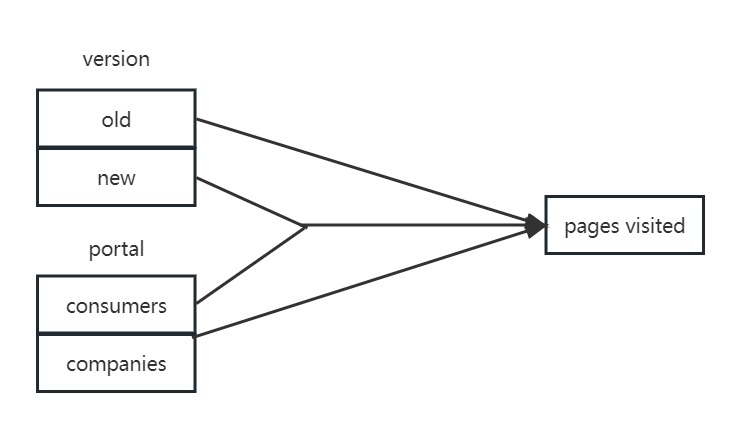
\includegraphics{CM.jpg}
\end{frame}

\begin{frame}{Specific Mathematical model}
\protect\hypertarget{specific-mathematical-model}{}
Describe the mathematical model that you fit on the data. Take for this
the complete model that you fit on the data. Also, explain your
selection for the priors. Assume Gaussian distribution for the number of
page visits.

I adopt linear regression model o fit the data, which can be expressed
as follows:

y = β₀ + β₁ * version + β₂ * portal + β₃ * version * portal + ε

\begin{itemize}
\tightlist
\item
  y represents the number of page visits, which is assumed to follow a
  Gaussian distribution.
\item
  version is a binary variable (0 for the old version, 1 for the new
  version) indicating the website version.
\item
  portal is a binary variable (0 for consumers, 1 for companies)
  indicating the web portal entry.
\item
  version * portal represents the interaction term between the website
  version and portal.
\item
  β₀ is intercept and β₁, β₂, and β₃ are the coefficients for the three
  terms. I adopt Cauchy distribution for them assuming weakly
  informative prior, which has a large scale value has a gentle slope,
  letting data in the more extreme region still be of influence if the
  likelihood is strong here
\item
  ε represents the error term, assumed to follow a Gaussian
  distribution, ε∼ Normal(0, σ).
\end{itemize}
\end{frame}

\begin{frame}[fragile]{Create Synthetic data}
\protect\hypertarget{create-synthetic-data}{}
Create a synthetic data set with a clear interaction effect between the
two factors for verifying your analysis later on. Report the values of
the coefficients of the linear model used to generate synthetic data.

\begin{Shaded}
\begin{Highlighting}[]
\CommentTok{\#include your code for generating the synthetic data}

\CommentTok{\# Set the seed for reproducibility}
\FunctionTok{set.seed}\NormalTok{(}\DecValTok{1}\NormalTok{)}

\CommentTok{\# Specify the sample size}
\NormalTok{n }\OtherTok{\textless{}{-}} \DecValTok{100}

\CommentTok{\# Create the independent variables}
\NormalTok{version }\OtherTok{\textless{}{-}} \FunctionTok{rep}\NormalTok{(}\FunctionTok{c}\NormalTok{(}\DecValTok{0}\NormalTok{, }\DecValTok{1}\NormalTok{), }\AttributeTok{each =}\NormalTok{ n}\SpecialCharTok{/}\DecValTok{2}\NormalTok{)}
\NormalTok{portal }\OtherTok{\textless{}{-}} \FunctionTok{rep}\NormalTok{(}\FunctionTok{c}\NormalTok{(}\DecValTok{0}\NormalTok{, }\DecValTok{1}\NormalTok{), }\AttributeTok{times =}\NormalTok{ n}\SpecialCharTok{/}\DecValTok{2}\NormalTok{)}

\CommentTok{\# Generate the interaction effect}
\NormalTok{interaction }\OtherTok{\textless{}{-}}\NormalTok{ version }\SpecialCharTok{*}\NormalTok{ portal}

\CommentTok{\# the values of the coefficients of the linear model}
\NormalTok{beta0 }\OtherTok{\textless{}{-}} \FloatTok{2.5}     \CommentTok{\# Intercept}
\NormalTok{beta1 }\OtherTok{\textless{}{-}} \FloatTok{1.5}     \CommentTok{\# Coefficient for version}
\NormalTok{beta2 }\OtherTok{\textless{}{-}} \FloatTok{0.8}     \CommentTok{\# Coefficient for portal}
\NormalTok{beta3 }\OtherTok{\textless{}{-}} \FloatTok{0.7}     \CommentTok{\# Coefficient for interaction}

\CommentTok{\# Generate the dependent variable (number of page visits)}
\NormalTok{page\_visits }\OtherTok{\textless{}{-}}\NormalTok{ beta0 }\SpecialCharTok{+}\NormalTok{ beta1 }\SpecialCharTok{*}\NormalTok{ version }\SpecialCharTok{+}\NormalTok{ beta2 }\SpecialCharTok{*}\NormalTok{ portal }\SpecialCharTok{+}\NormalTok{ beta3 }\SpecialCharTok{*}\NormalTok{ interaction }\SpecialCharTok{+} \FunctionTok{rnorm}\NormalTok{(n)}

\CommentTok{\# Combine the variables into a data frame}
\NormalTok{data }\OtherTok{\textless{}{-}} \FunctionTok{data.frame}\NormalTok{(version, portal, interaction, page\_visits)}

\CommentTok{\# View the first few rows of the synthetic data set}
\FunctionTok{head}\NormalTok{(data)}
\end{Highlighting}
\end{Shaded}

\begin{verbatim}
##   version portal interaction page_visits
## 1       0      0           0    1.873546
## 2       0      1           0    3.483643
## 3       0      0           0    1.664371
## 4       0      1           0    4.895281
## 5       0      0           0    2.829508
## 6       0      1           0    2.479532
\end{verbatim}
\end{frame}

\begin{frame}[fragile]{Visual inspection}
\protect\hypertarget{visual-inspection}{}
Graphically examine the mean page visits for the four different
conditions. Give a short explanation of the figure.

\begin{Shaded}
\begin{Highlighting}[]
\CommentTok{\#include your code and output in the document}

\CommentTok{\# Load the required library}
\FunctionTok{library}\NormalTok{(ggplot2)}
\end{Highlighting}
\end{Shaded}

\begin{verbatim}
## 
## Attaching package: 'ggplot2'
\end{verbatim}

\begin{verbatim}
## The following object is masked from 'package:NLP':
## 
##     annotate
\end{verbatim}

\begin{Shaded}
\begin{Highlighting}[]
\CommentTok{\# Compute the mean page visits for each condition}
\NormalTok{mean\_data }\OtherTok{\textless{}{-}} \FunctionTok{aggregate}\NormalTok{(page\_visits }\SpecialCharTok{\textasciitilde{}}\NormalTok{ version }\SpecialCharTok{+}\NormalTok{ portal, data, mean)}

\CommentTok{\# Create a grouped bar plot}
\FunctionTok{ggplot}\NormalTok{(mean\_data, }\FunctionTok{aes}\NormalTok{(}\AttributeTok{x =}\NormalTok{ version, }\AttributeTok{y =}\NormalTok{ page\_visits, }\AttributeTok{fill =} \FunctionTok{factor}\NormalTok{(portal))) }\SpecialCharTok{+}
  \FunctionTok{geom\_bar}\NormalTok{(}\AttributeTok{stat =} \StringTok{"identity"}\NormalTok{, }\AttributeTok{position =} \StringTok{"dodge"}\NormalTok{) }\SpecialCharTok{+}
  \FunctionTok{labs}\NormalTok{(}\AttributeTok{x =} \StringTok{"Website Version"}\NormalTok{, }\AttributeTok{y =} \StringTok{"Mean Page Visits"}\NormalTok{) }\SpecialCharTok{+}
  \FunctionTok{scale\_fill\_discrete}\NormalTok{(}\AttributeTok{name =} \StringTok{"Portal"}\NormalTok{) }\SpecialCharTok{+}
  \FunctionTok{theme\_bw}\NormalTok{()}
\end{Highlighting}
\end{Shaded}

\includegraphics{Markdown-report-template-assignmentA-2023Q4_files/figure-beamer/unnamed-chunk-11-1.pdf}

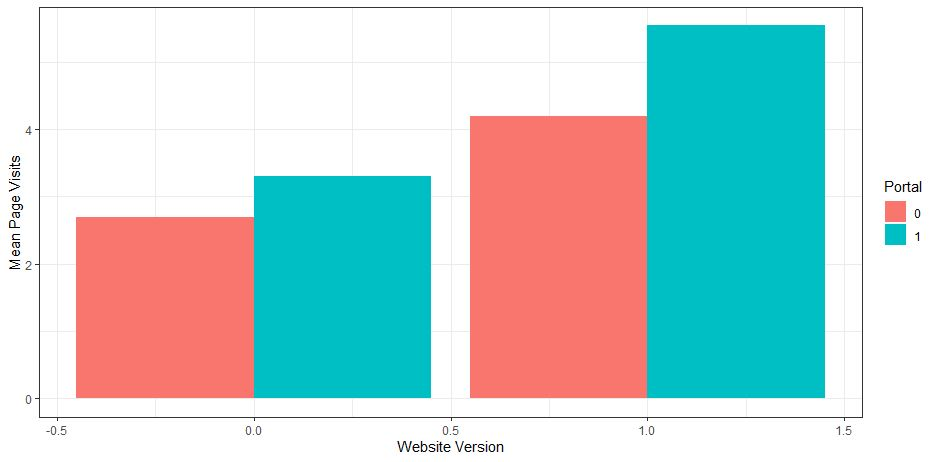
\includegraphics{visual_inspection_2.jpg}

I conducted a simple effect analysis to examine the influence of one
independent variable on different levels of another independent
variable. The analysis revealed that the combination of the new version
and web portal for companies resulted in a highest number of page
visits. Furthermore, regardless of the website version, the portal for
companies showed a higher number of page visits compared to the portal
for consumers. Additionally, irrespective of the portal, the old version
exhibited fewer page visits compared to the new version.
\end{frame}

\begin{frame}[fragile]{Frequentist Approach}
\protect\hypertarget{frequentist-approach-1}{}
\begin{block}{Model verification}
\protect\hypertarget{model-verification}{}
Verify your model analysis with synthetic data and show that it can
reproduce the coefficients of the linear model that you used to generate
the synthetic data set. Provide a short interpretation of the results,
with a reflection of AICc, F-value, p-value etc.

\begin{Shaded}
\begin{Highlighting}[]
\CommentTok{\#include your analysis code of synthetic data and output in the document}

\CommentTok{\# Fit the linear regression model}
\NormalTok{model }\OtherTok{\textless{}{-}} \FunctionTok{lm}\NormalTok{(page\_visits }\SpecialCharTok{\textasciitilde{}}\NormalTok{ version }\SpecialCharTok{+}\NormalTok{ portal }\SpecialCharTok{+}\NormalTok{ interaction, }\AttributeTok{data =}\NormalTok{ data)}

\CommentTok{\# Print the model summary}
\FunctionTok{summary}\NormalTok{(model)}
\end{Highlighting}
\end{Shaded}

\begin{verbatim}
## 
## Call:
## lm(formula = page_visits ~ version + portal + interaction, data = data)
## 
## Residuals:
##      Min       1Q   Median       3Q      Max 
## -2.21954 -0.63146 -0.02511  0.56114  2.20663 
## 
## Coefficients:
##             Estimate Std. Error t value Pr(>|t|)    
## (Intercept)   2.6961     0.1815  14.850  < 2e-16 ***
## version       1.4989     0.2567   5.838 7.16e-08 ***
## portal        0.6088     0.2567   2.371   0.0197 *  
## interaction   0.7359     0.3631   2.027   0.0455 *  
## ---
## Signif. codes:  0 '***' 0.001 '**' 0.01 '*' 0.05 '.' 0.1 ' ' 1
## 
## Residual standard error: 0.9077 on 96 degrees of freedom
## Multiple R-squared:  0.5911, Adjusted R-squared:  0.5784 
## F-statistic: 46.26 on 3 and 96 DF,  p-value: < 2.2e-16
\end{verbatim}

\begin{Shaded}
\begin{Highlighting}[]
\CommentTok{\# Calculate AIC}
\NormalTok{AIC }\OtherTok{\textless{}{-}} \FunctionTok{AIC}\NormalTok{(model)}

\CommentTok{\# Calculate the number of parameters}
\NormalTok{k }\OtherTok{\textless{}{-}} \FunctionTok{length}\NormalTok{(}\FunctionTok{coef}\NormalTok{(model))}

\CommentTok{\# Calculate the AICc}
\NormalTok{n }\OtherTok{\textless{}{-}} \FunctionTok{nrow}\NormalTok{(data)}
\NormalTok{AICc }\OtherTok{\textless{}{-}}\NormalTok{ AIC }\SpecialCharTok{+}\NormalTok{ (}\DecValTok{2} \SpecialCharTok{*}\NormalTok{ k }\SpecialCharTok{*}\NormalTok{ (k }\SpecialCharTok{+} \DecValTok{1}\NormalTok{)) }\SpecialCharTok{/}\NormalTok{ (n }\SpecialCharTok{{-}}\NormalTok{ k }\SpecialCharTok{{-}} \DecValTok{1}\NormalTok{)}


\CommentTok{\# Print the results}
\FunctionTok{cat}\NormalTok{(}\StringTok{"Coefficients:}\SpecialCharTok{\textbackslash{}n}\StringTok{"}\NormalTok{)}
\end{Highlighting}
\end{Shaded}

\begin{verbatim}
## Coefficients:
\end{verbatim}

\begin{Shaded}
\begin{Highlighting}[]
\FunctionTok{print}\NormalTok{(}\FunctionTok{coef}\NormalTok{(model))}
\end{Highlighting}
\end{Shaded}

\begin{verbatim}
## (Intercept)     version      portal interaction 
##   2.6960603   1.4989306   0.6087760   0.7358952
\end{verbatim}

\begin{Shaded}
\begin{Highlighting}[]
\FunctionTok{cat}\NormalTok{(}\StringTok{"}\SpecialCharTok{\textbackslash{}n}\StringTok{AIC:"}\NormalTok{, AIC)}
\end{Highlighting}
\end{Shaded}

\begin{verbatim}
## 
## AIC: 270.3466
\end{verbatim}

\begin{Shaded}
\begin{Highlighting}[]
\FunctionTok{cat}\NormalTok{(}\StringTok{"}\SpecialCharTok{\textbackslash{}n}\StringTok{AICc:"}\NormalTok{, AICc)}
\end{Highlighting}
\end{Shaded}

\begin{verbatim}
## 
## AICc: 270.7676
\end{verbatim}

\begin{Shaded}
\begin{Highlighting}[]
\CommentTok{\#result:}

\CommentTok{\#Coefficients:}
\CommentTok{\#            Estimate Std. Error t value Pr(\textgreater{}|t|)    }
\CommentTok{\#(Intercept)   2.6961     0.1815  14.850  \textless{} 2e{-}16 ***}
\CommentTok{\#version       1.4989     0.2567   5.838 7.16e{-}08 ***}
\CommentTok{\#portal        0.6088     0.2567   2.371   0.0197 *  }
\CommentTok{\#interaction   0.7359     0.3631   2.027   0.0455 *  }

\CommentTok{\#F{-}statistic: 46.26 on 3 and 96 DF,  p{-}value: \textless{} 2.2e{-}16}

\CommentTok{\#AIC: 270.3466}

\CommentTok{\#AICc: 270.7676}

\CommentTok{\#interpretation}
\CommentTok{\#1. All coefficients are comparable to original values and statistically significant.}
\CommentTok{\#2. The p{-}value is reported as "\textless{} 2.2e{-}16", which is essentially zero. This extremely low p{-}value indicates strong evidence against the null hypothesis, suggesting that the predictors collectively have a significant effect on the outcome variable (page visits).}
\CommentTok{\#3. The AICc value of 270.3466 suggests that the fitted linear regression model has a relatively good fit to the data compared to alternative models.}
\end{Highlighting}
\end{Shaded}
\end{block}

\begin{block}{Model analysis with Gaussian distribution assumed}
\protect\hypertarget{model-analysis-with-gaussian-distribution-assumed}{}
Redo the analysis now on the real data set. Assume Gaussian distribution
for the number of page visits. Provide a short interpretation of the
results, with an interpretation of AICc, F-value, p-value, etc.

\begin{Shaded}
\begin{Highlighting}[]
\CommentTok{\#include your code and output in the document}

\CommentTok{\#include your analysis code of synthetic data and output in the document}

\CommentTok{\#set work path}

\CommentTok{\#read data and add interaction}
\NormalTok{web\_data }\OtherTok{\textless{}{-}} \FunctionTok{read.csv}\NormalTok{(}\StringTok{"data/webvisit0.csv"}\NormalTok{) }
\NormalTok{web\_data}\SpecialCharTok{$}\NormalTok{interaction }\OtherTok{\textless{}{-}}\NormalTok{ web\_data}\SpecialCharTok{$}\NormalTok{version }\SpecialCharTok{*}\NormalTok{ web\_data}\SpecialCharTok{$}\NormalTok{portal}

\CommentTok{\# Fit the linear regression model}
\NormalTok{model0 }\OtherTok{\textless{}{-}} \FunctionTok{lm}\NormalTok{(pages }\SpecialCharTok{\textasciitilde{}}\NormalTok{ version }\SpecialCharTok{+}\NormalTok{ portal }\SpecialCharTok{+}\NormalTok{ interaction, }\AttributeTok{data =}\NormalTok{ web\_data)}

\CommentTok{\# Print the model summary}
\FunctionTok{summary}\NormalTok{(model0)}
\end{Highlighting}
\end{Shaded}

\begin{verbatim}
## 
## Call:
## lm(formula = pages ~ version + portal + interaction, data = web_data)
## 
## Residuals:
##      Min       1Q   Median       3Q      Max 
## -17.3511  -3.3511  -0.0943   3.3720  21.6489 
## 
## Coefficients:
##             Estimate Std. Error t value Pr(>|t|)    
## (Intercept)  19.6280     0.3443   57.02   <2e-16 ***
## version      -7.6239     0.4898  -15.56   <2e-16 ***
## portal       13.4663     0.4898   27.49   <2e-16 ***
## interaction  29.8808     0.6888   43.38   <2e-16 ***
## ---
## Signif. codes:  0 '***' 0.001 '**' 0.01 '*' 0.05 '.' 0.1 ' ' 1
## 
## Residual standard error: 5.443 on 996 degrees of freedom
## Multiple R-squared:  0.9036, Adjusted R-squared:  0.9033 
## F-statistic:  3110 on 3 and 996 DF,  p-value: < 2.2e-16
\end{verbatim}

\begin{Shaded}
\begin{Highlighting}[]
\CommentTok{\#result:}

\CommentTok{\#Coefficients:}
\CommentTok{\#            Estimate Std. Error t value Pr(\textgreater{}|t|)    }
\CommentTok{\#(Intercept)  19.6280     0.3443   57.02   \textless{}2e{-}16 ***}
\CommentTok{\#version      {-}7.6239     0.4898  {-}15.56   \textless{}2e{-}16 ***}
\CommentTok{\#portal       13.4663     0.4898   27.49   \textless{}2e{-}16 ***}
\CommentTok{\#interaction  29.8808     0.6888   43.38   \textless{}2e{-}16 ***}

\CommentTok{\#F{-}statistic:  3110 on 3 and 996 DF,  p{-}value: \textless{} 2.2e{-}16}

\CommentTok{\#interpretation}
\CommentTok{\#1. All coefficients are statistically significant, which show that version, portal and interaction have a strong influence on the page visit.}
\CommentTok{\#2. The p{-}value is reported as "\textless{} 2.2e{-}16", which is essentially zero. This extremely low p{-}value indicates strong evidence against the null hypothesis, suggesting that the predictors collectively have a significant effect on the outcome variable (page visits).}
\end{Highlighting}
\end{Shaded}
\end{block}

\begin{block}{Assumption analysis}
\protect\hypertarget{assumption-analysis}{}
Redo the analysis on the real tweet data set. This time assume a Poisson
distribution for the number of page visits. For the best fitting models
(Gaussian and Poisson), examine graphically the distribution of the
residuals for the model that assumes Gaussian distribution and the model
that assumes Poisson distribution. Give a brief interpretation of
Poisson and Gaussian distribution assumptions.

\begin{Shaded}
\begin{Highlighting}[]
\CommentTok{\#include your code and output in the document}

\CommentTok{\# Poisson regression}
\NormalTok{poisson\_model }\OtherTok{\textless{}{-}} \FunctionTok{glm}\NormalTok{(pages }\SpecialCharTok{\textasciitilde{}}\NormalTok{ version }\SpecialCharTok{+}\NormalTok{ portal }\SpecialCharTok{+}\NormalTok{ interaction, }\AttributeTok{data =}\NormalTok{ web\_data, }\AttributeTok{family =}\NormalTok{ poisson)}

\CommentTok{\# Gaussian regression}
\NormalTok{gaussian\_model }\OtherTok{\textless{}{-}}\NormalTok{ model0}

\CommentTok{\# Residual analysis}
\NormalTok{poisson\_residuals }\OtherTok{\textless{}{-}} \FunctionTok{resid}\NormalTok{(poisson\_model)}
\NormalTok{gaussian\_residuals }\OtherTok{\textless{}{-}} \FunctionTok{resid}\NormalTok{(gaussian\_model)}

\CommentTok{\# Histogram of Poisson model residuals}
\FunctionTok{hist}\NormalTok{(poisson\_residuals, }\AttributeTok{breaks =} \DecValTok{30}\NormalTok{, }\AttributeTok{col =} \StringTok{"lightblue"}\NormalTok{, }\AttributeTok{main =} \StringTok{"Poisson Model Residuals"}\NormalTok{)}
\end{Highlighting}
\end{Shaded}

\includegraphics{Markdown-report-template-assignmentA-2023Q4_files/figure-beamer/unnamed-chunk-14-1.pdf}

\begin{Shaded}
\begin{Highlighting}[]
\CommentTok{\# Density plot of Gaussian model residuals}
\FunctionTok{hist}\NormalTok{(gaussian\_residuals, }\AttributeTok{breaks =} \DecValTok{30}\NormalTok{, }\AttributeTok{col =} \StringTok{"lightblue"}\NormalTok{, }\AttributeTok{main =} \StringTok{"Gaussian Model Residuals"}\NormalTok{)}
\end{Highlighting}
\end{Shaded}

\includegraphics{Markdown-report-template-assignmentA-2023Q4_files/figure-beamer/unnamed-chunk-14-2.pdf}

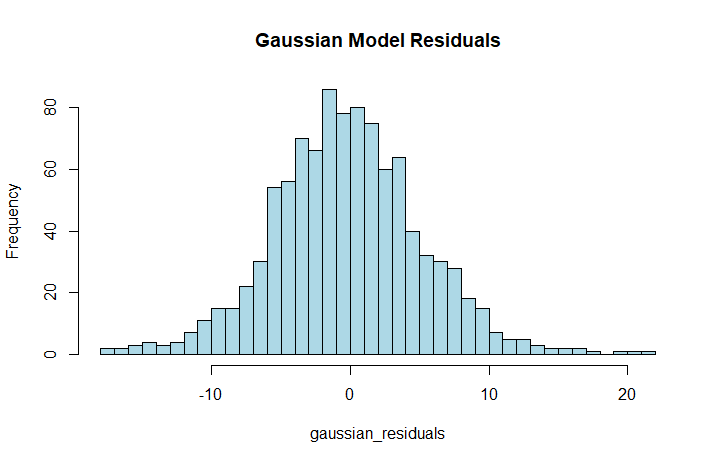
\includegraphics{gaussian.jpg}

\begin{figure}
\centering
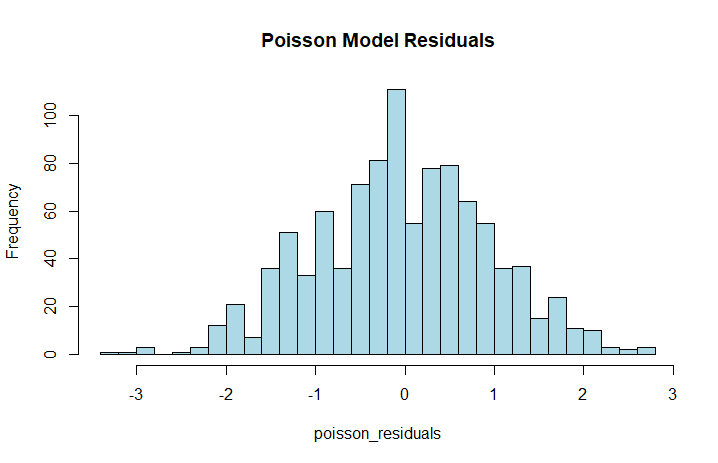
\includegraphics{poisson.jpg}
\caption{poisson}
\end{figure}

Both the Gaussian and Poisson residuals appear to follow a normal
distribution, which suggests that the Gaussian model is a better fit for
the data.
\end{block}

\begin{block}{Simple effect analysis}
\protect\hypertarget{simple-effect-analysis}{}
Continue with the model that assumes a Poisson distribution. If the
analysis shows a significant two-way interaction effect, conduct a
Simple Effect analysis to explore this interaction effect in more
detail. Provide a brief interpretation of the results.

\begin{Shaded}
\begin{Highlighting}[]
\CommentTok{\#include your code and output in the document}

\FunctionTok{library}\NormalTok{(rethinking)}
\FunctionTok{summary}\NormalTok{(poisson\_model)}
\end{Highlighting}
\end{Shaded}

\begin{verbatim}
## 
## Call:
## glm(formula = pages ~ version + portal + interaction, family = poisson, 
##     data = web_data)
## 
## Coefficients:
##             Estimate Std. Error z value Pr(>|z|)    
## (Intercept)  2.97696    0.01428  208.54   <2e-16 ***
## version     -0.49171    0.02335  -21.06   <2e-16 ***
## portal       0.52240    0.01810   28.86   <2e-16 ***
## interaction  1.00605    0.02717   37.03   <2e-16 ***
## ---
## Signif. codes:  0 '***' 0.001 '**' 0.01 '*' 0.05 '.' 0.1 ' ' 1
## 
## (Dispersion parameter for poisson family taken to be 1)
## 
##     Null deviance: 9959.66  on 999  degrees of freedom
## Residual deviance:  970.17  on 996  degrees of freedom
## AIC: 6057.5
## 
## Number of Fisher Scoring iterations: 4
\end{verbatim}

\begin{Shaded}
\begin{Highlighting}[]
\CommentTok{\# interaction  1.00605    0.02717   37.03   \textless{}2e{-}16 ***}
\CommentTok{\# The p{-}value is reported as "\textless{} 2.2e{-}16", which is essentially zero. This extremely low p{-}value indicates strong evidence against the null hypothesis, suggesting that the interaction have a significant effect on the page visits.}

\FunctionTok{library}\NormalTok{(pander)}

\CommentTok{\# create two contrasts and combine them and associate the contrast to a variable}
\NormalTok{web\_data}\SpecialCharTok{$}\NormalTok{simple }\OtherTok{\textless{}{-}} \FunctionTok{interaction}\NormalTok{(web\_data}\SpecialCharTok{$}\NormalTok{version, web\_data}\SpecialCharTok{$}\NormalTok{portal) }\CommentTok{\#merge two factors}
\FunctionTok{levels}\NormalTok{(web\_data}\SpecialCharTok{$}\NormalTok{simple) }\CommentTok{\#to see the level in the new factor}
\end{Highlighting}
\end{Shaded}

\begin{verbatim}
## [1] "0.0" "1.0" "0.1" "1.1"
\end{verbatim}

\begin{Shaded}
\begin{Highlighting}[]
\NormalTok{contrastOld }\OtherTok{\textless{}{-}}\FunctionTok{c}\NormalTok{(}\DecValTok{1}\NormalTok{,}\SpecialCharTok{{-}}\DecValTok{1}\NormalTok{,}\DecValTok{0}\NormalTok{,}\DecValTok{0}\NormalTok{) }
\NormalTok{contrastNew }\OtherTok{\textless{}{-}}\FunctionTok{c}\NormalTok{(}\DecValTok{0}\NormalTok{,}\DecValTok{0}\NormalTok{,}\DecValTok{1}\NormalTok{,}\SpecialCharTok{{-}}\DecValTok{1}\NormalTok{) }

\NormalTok{SimpleEff }\OtherTok{\textless{}{-}} \FunctionTok{cbind}\NormalTok{(contrastOld,contrastNew)}
\FunctionTok{contrasts}\NormalTok{(web\_data}\SpecialCharTok{$}\NormalTok{simple) }\OtherTok{\textless{}{-}}\NormalTok{ SimpleEff }\CommentTok{\#now we link the two contrasts with the version}

\CommentTok{\# we fit a linear model on the data, using this two{-}level variable as an independent factor.}
\NormalTok{simpleEffectModel }\OtherTok{\textless{}{-}}\FunctionTok{lm}\NormalTok{(pages }\SpecialCharTok{\textasciitilde{}}\NormalTok{ simple , }\AttributeTok{data =}\NormalTok{ web\_data, }\AttributeTok{na.action =}\NormalTok{ na.exclude)}
\FunctionTok{pander}\NormalTok{(}\FunctionTok{summary.lm}\NormalTok{(simpleEffectModel))}
\end{Highlighting}
\end{Shaded}

\begin{longtable}[]{@{}
  >{\centering\arraybackslash}p{(\columnwidth - 8\tabcolsep) * \real{0.3333}}
  >{\centering\arraybackslash}p{(\columnwidth - 8\tabcolsep) * \real{0.1528}}
  >{\centering\arraybackslash}p{(\columnwidth - 8\tabcolsep) * \real{0.1806}}
  >{\centering\arraybackslash}p{(\columnwidth - 8\tabcolsep) * \real{0.1389}}
  >{\centering\arraybackslash}p{(\columnwidth - 8\tabcolsep) * \real{0.1806}}@{}}
\toprule()
\begin{minipage}[b]{\linewidth}\centering
~
\end{minipage} & \begin{minipage}[b]{\linewidth}\centering
Estimate
\end{minipage} & \begin{minipage}[b]{\linewidth}\centering
Std. Error
\end{minipage} & \begin{minipage}[b]{\linewidth}\centering
t value
\end{minipage} & \begin{minipage}[b]{\linewidth}\centering
Pr(\textgreater\textbar t\textbar)
\end{minipage} \\
\midrule()
\endhead
\textbf{(Intercept)} & 30.02 & 0.1722 & 174.3 & 0 \\
\textbf{simplecontrastOld} & 3.812 & 0.2449 & 15.56 & 4.691e-49 \\
\textbf{simplecontrastNew} & -11.13 & 0.2421 & -45.96 & 2.195e-248 \\
\textbf{simple} & 28.41 & 0.3444 & 82.48 & 0 \\
\bottomrule()
\end{longtable}

\begin{longtable}[]{@{}
  >{\centering\arraybackslash}p{(\columnwidth - 6\tabcolsep) * \real{0.2083}}
  >{\centering\arraybackslash}p{(\columnwidth - 6\tabcolsep) * \real{0.3056}}
  >{\centering\arraybackslash}p{(\columnwidth - 6\tabcolsep) * \real{0.1250}}
  >{\centering\arraybackslash}p{(\columnwidth - 6\tabcolsep) * \real{0.2361}}@{}}
\caption{Fitting linear model: pages \textasciitilde{}
simple}\tabularnewline
\toprule()
\begin{minipage}[b]{\linewidth}\centering
Observations
\end{minipage} & \begin{minipage}[b]{\linewidth}\centering
Residual Std. Error
\end{minipage} & \begin{minipage}[b]{\linewidth}\centering
\(R^2\)
\end{minipage} & \begin{minipage}[b]{\linewidth}\centering
Adjusted \(R^2\)
\end{minipage} \\
\midrule()
\endfirsthead
\toprule()
\begin{minipage}[b]{\linewidth}\centering
Observations
\end{minipage} & \begin{minipage}[b]{\linewidth}\centering
Residual Std. Error
\end{minipage} & \begin{minipage}[b]{\linewidth}\centering
\(R^2\)
\end{minipage} & \begin{minipage}[b]{\linewidth}\centering
Adjusted \(R^2\)
\end{minipage} \\
\midrule()
\endhead
1000 & 5.443 & 0.9036 & 0.9033 \\
\bottomrule()
\end{longtable}

\begin{Shaded}
\begin{Highlighting}[]
\CommentTok{\# result:}
\CommentTok{\#{-}{-}{-}{-}{-}{-}{-}{-}{-}{-}{-}{-}{-}{-}{-}{-}{-}{-}{-}{-}{-}{-}{-}{-}{-}{-}{-}{-}{-}{-}{-}{-}{-}{-}{-}{-}{-}{-}{-}{-}{-}{-}{-}{-}{-}{-}{-}{-}{-}{-}{-}{-}{-}{-}{-}{-}{-}{-}{-}{-}{-}{-}{-}{-}{-}{-}{-}{-}{-}{-}}
\CommentTok{\#        \&nbsp;           Estimate   Std. Error   t value    Pr(\textgreater{}|t|)  }
\CommentTok{\#{-}{-}{-}{-}{-}{-}{-}{-}{-}{-}{-}{-}{-}{-}{-}{-}{-}{-}{-}{-}{-}{-}{-} {-}{-}{-}{-}{-}{-}{-}{-}{-}{-} {-}{-}{-}{-}{-}{-}{-}{-}{-}{-}{-}{-} {-}{-}{-}{-}{-}{-}{-}{-}{-} {-}{-}{-}{-}{-}{-}{-}{-}{-}{-}{-}{-}}
\CommentTok{\#    **(Intercept)**       30.02       0.1722      174.3        0      }
\CommentTok{\#}
\CommentTok{\# **simplecontrastOld**    3.812       0.2449      15.56    4.691e{-}49  }

\CommentTok{\# **simplecontrastNew**    {-}11.13      0.2421     {-}45.96    2.195e{-}248 }

\CommentTok{\#      **simple**          28.41       0.3444      82.48        0      }
\CommentTok{\#{-}{-}{-}{-}{-}{-}{-}{-}{-}{-}{-}{-}{-}{-}{-}{-}{-}{-}{-}{-}{-}{-}{-}{-}{-}{-}{-}{-}{-}{-}{-}{-}{-}{-}{-}{-}{-}{-}{-}{-}{-}{-}{-}{-}{-}{-}{-}{-}{-}{-}{-}{-}{-}{-}{-}{-}{-}{-}{-}{-}{-}{-}{-}{-}{-}{-}{-}{-}{-}{-}}

\CommentTok{\# It revealed a significant (t = 15.56, p. \textless{} 0.01) difference for old version in page visits, and also a significant effect (t = {-}45.96,p. \textless{} 0.01 ) was found for the onew version in page visits.}
\end{Highlighting}
\end{Shaded}
\end{block}

\begin{block}{Report section for a scientific publication}
\protect\hypertarget{report-section-for-a-scientific-publication-1}{}
Write a small section for a scientific publication, in which you report
the results of the analyses, and explain the conclusions that can be
drawn.

Paper:
\href{https://www.sciencedirect.com/science/article/pii/S1071581916000392}{Effects
of different real-time feedback types on human performance in
high-demanding work conditions}

Result:

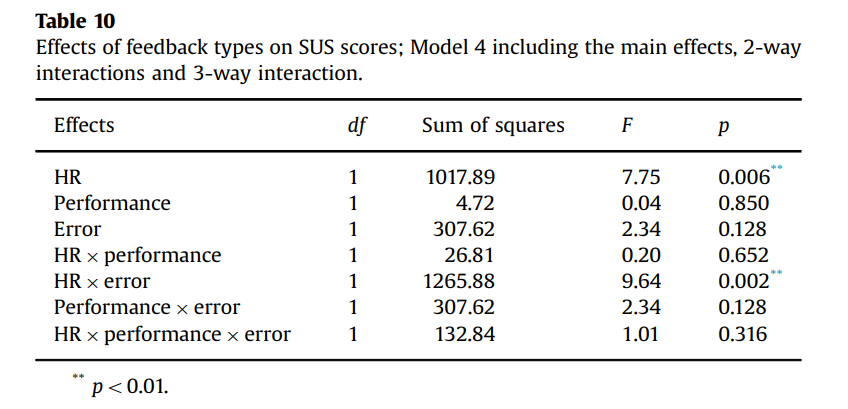
\includegraphics{table.jpg}

The table shows the simple effect of HR, performance and error as well
as the 2-way/3-way interaction between/among them. We can see from the
table that there is a significant two-way interaction effect between HR
and Error.(p\textless0.002) Also, the HR itself is a significant
effect(p\textless0,006).
\end{block}
\end{frame}

\begin{frame}[fragile]{Bayesian Approach}
\protect\hypertarget{bayesian-approach-1}{}
For the Bayesian analyses, use the rethinking and/or BayesianFirstAid
library

\begin{block}{Verification Analysis}
\protect\hypertarget{verification-analysis}{}
Verify your model analysis with synthetic data and show that it can
reproduce the coefficients of the linear model that you used to generate
the synthetic data set. Provide a short interpretation of the results,
with a reflection of WAIC, and 95\% credibility interval of coefficients
for individual celebrities.

\begin{Shaded}
\begin{Highlighting}[]
\CommentTok{\#include your analysis code of synthetic data and output in the document}
\FunctionTok{library}\NormalTok{(rethinking)}

\NormalTok{model\_bay\_fake }\OtherTok{\textless{}{-}} \FunctionTok{map}\NormalTok{(}
  \FunctionTok{alist}\NormalTok{(}
\NormalTok{    page\_visits }\SpecialCharTok{\textasciitilde{}} \FunctionTok{dnorm}\NormalTok{(mu, sigma),}
\NormalTok{    mu }\OtherTok{\textless{}{-}}\NormalTok{ beta0 }\SpecialCharTok{+}\NormalTok{ beta1}\SpecialCharTok{*}\NormalTok{version }\SpecialCharTok{+}\NormalTok{ beta2}\SpecialCharTok{*}\NormalTok{portal }\SpecialCharTok{+}\NormalTok{ beta3}\SpecialCharTok{*}\NormalTok{interaction,}
\NormalTok{    beta0 }\SpecialCharTok{\textasciitilde{}} \FunctionTok{dnorm}\NormalTok{(}\DecValTok{0}\NormalTok{, }\DecValTok{10}\NormalTok{),}
\NormalTok{    beta1 }\SpecialCharTok{\textasciitilde{}} \FunctionTok{dnorm}\NormalTok{(}\DecValTok{0}\NormalTok{, }\DecValTok{10}\NormalTok{),}
\NormalTok{    beta2 }\SpecialCharTok{\textasciitilde{}} \FunctionTok{dnorm}\NormalTok{(}\DecValTok{0}\NormalTok{, }\DecValTok{10}\NormalTok{),}
\NormalTok{    beta3 }\SpecialCharTok{\textasciitilde{}} \FunctionTok{dnorm}\NormalTok{(}\DecValTok{0}\NormalTok{, }\DecValTok{10}\NormalTok{),}
\NormalTok{    sigma }\SpecialCharTok{\textasciitilde{}} \FunctionTok{dcauchy}\NormalTok{(}\DecValTok{0}\NormalTok{, }\FloatTok{2.5}\NormalTok{)}
\NormalTok{  ),}
  \AttributeTok{data =}\NormalTok{ data,}
  \AttributeTok{start =} \FunctionTok{list}\NormalTok{(}\AttributeTok{beta0 =} \FloatTok{2.5}\NormalTok{, }\AttributeTok{beta1 =} \FloatTok{1.5}\NormalTok{, }\AttributeTok{beta2 =} \FloatTok{0.8}\NormalTok{, }\AttributeTok{beta3 =} \FloatTok{0.7}\NormalTok{, }\AttributeTok{sigma =} \DecValTok{1}\NormalTok{)}
\NormalTok{)}


\FunctionTok{precis}\NormalTok{(model\_bay\_fake, }\AttributeTok{prob =}\NormalTok{ .}\DecValTok{95}\NormalTok{)}
\end{Highlighting}
\end{Shaded}

\begin{verbatim}
##            mean        sd       2.5%    97.5%
## beta0 2.6956423 0.1775695 2.34761243 3.043672
## beta1 1.4991075 0.2510816 1.00699650 1.991218
## beta2 0.6092341 0.2510817 0.11712314 1.101345
## beta3 0.7354461 0.3550131 0.03963326 1.431259
## sigma 0.8884077 0.0626871 0.76554325 1.011272
\end{verbatim}

\begin{Shaded}
\begin{Highlighting}[]
\NormalTok{waic }\OtherTok{\textless{}{-}} \FunctionTok{WAIC}\NormalTok{(model\_bay\_fake)}
\NormalTok{waic}
\end{Highlighting}
\end{Shaded}

\begin{verbatim}
##       WAIC      lppd  penalty  std_err
## 1 271.6464 -130.2559 5.567342 15.19836
\end{verbatim}

\begin{Shaded}
\begin{Highlighting}[]
\CommentTok{\#Result}
\CommentTok{\#      mean   sd 2.5\% 97.5\%}
\CommentTok{\#beta0 2.70 0.18 2.35  3.04}
\CommentTok{\#beta1 1.50 0.25 1.01  1.99}
\CommentTok{\#beta2 0.61 0.25 0.12  1.10}
\CommentTok{\#beta3 0.74 0.36 0.04  1.43}
\CommentTok{\#sigma 0.89 0.06 0.77  1.01}

\CommentTok{\#      WAIC      lppd  penalty  std\_err}
\CommentTok{\#1 271.2522 {-}130.2396 5.386505 15.16342}

\CommentTok{\# The estimated coefficients of the synthetic data closely match the original coefficients used to generate the data, with portal, version and interaction all positively affect the page visit.}
\end{Highlighting}
\end{Shaded}
\end{block}

\begin{block}{Model description}
\protect\hypertarget{model-description-1}{}
Describe the mathematical model fitted on the most extensive model.
(hint, look at the mark down file of the lectures to see example on
formulate mathematical models in markdown). Assume Poisson distribution
for the number of page visits. Justify the priors.

Model:

Pages \textasciitilde{} Poisson(lambda)

lambda = exp(beta0 + beta1 * Version + beta2 * Portal + beta3 *
Interaction)

Priors:

Because there is limited prior information or no strong prior beliefs, I
use weakly informative priors that allow the data to have a larger
influence on the posterior results.

\begin{itemize}
\tightlist
\item
  beta0 \textasciitilde{} Normal(0, 10)
\item
  beta1 \textasciitilde{} Normal(0, 10)
\item
  beta2 \textasciitilde{} Normal(0, 10)
\item
  beta3 \textasciitilde{} Normal(0, 10)
\end{itemize}
\end{block}

\begin{block}{Model comparison}
\protect\hypertarget{model-comparison-1}{}
Redo the analysis on actual data. Assume Poisson distribution for the
number of page visits. Provide brief interpretation of the analysis
results (e.g.~WAIC, and 95\% credibility interval of coefficients).

\begin{Shaded}
\begin{Highlighting}[]
\CommentTok{\#include your code and output in the document}

\CommentTok{\#set work path}

\CommentTok{\#read data and add interaction}
\NormalTok{web\_data }\OtherTok{\textless{}{-}} \FunctionTok{read.csv}\NormalTok{(}\StringTok{"data/webvisit0.csv"}\NormalTok{) }
\NormalTok{web\_data}\SpecialCharTok{$}\NormalTok{interaction }\OtherTok{\textless{}{-}}\NormalTok{ web\_data}\SpecialCharTok{$}\NormalTok{version }\SpecialCharTok{*}\NormalTok{ web\_data}\SpecialCharTok{$}\NormalTok{portal}

\FunctionTok{library}\NormalTok{(rethinking)}


\CommentTok{\# Model formulation}
\NormalTok{model\_bay\_web }\OtherTok{\textless{}{-}} \FunctionTok{map}\NormalTok{(}
  \FunctionTok{alist}\NormalTok{(}
\NormalTok{    pages }\SpecialCharTok{\textasciitilde{}} \FunctionTok{dpois}\NormalTok{(lambda),}
    \FunctionTok{log}\NormalTok{(lambda) }\OtherTok{\textless{}{-}}\NormalTok{ beta0 }\SpecialCharTok{+}\NormalTok{ beta1 }\SpecialCharTok{*}\NormalTok{ version }\SpecialCharTok{+}\NormalTok{ beta2 }\SpecialCharTok{*}\NormalTok{ portal }\SpecialCharTok{+}\NormalTok{ beta3 }\SpecialCharTok{*}\NormalTok{ interaction,}
\NormalTok{    beta0 }\SpecialCharTok{\textasciitilde{}} \FunctionTok{dnorm}\NormalTok{(}\DecValTok{0}\NormalTok{, }\DecValTok{10}\NormalTok{),}
\NormalTok{    beta1 }\SpecialCharTok{\textasciitilde{}} \FunctionTok{dnorm}\NormalTok{(}\DecValTok{0}\NormalTok{, }\DecValTok{10}\NormalTok{),}
\NormalTok{    beta2 }\SpecialCharTok{\textasciitilde{}} \FunctionTok{dnorm}\NormalTok{(}\DecValTok{0}\NormalTok{, }\DecValTok{10}\NormalTok{),}
\NormalTok{    beta3 }\SpecialCharTok{\textasciitilde{}} \FunctionTok{dnorm}\NormalTok{(}\DecValTok{0}\NormalTok{, }\DecValTok{10}\NormalTok{)}
\NormalTok{  ),}
  \AttributeTok{data =}\NormalTok{ web\_data,}
\NormalTok{)}

\FunctionTok{precis}\NormalTok{(model\_bay\_web, }\AttributeTok{prob =}\NormalTok{ .}\DecValTok{95}\NormalTok{)}
\end{Highlighting}
\end{Shaded}

\begin{verbatim}
##             mean         sd       2.5%      97.5%
## beta0  2.9771152 0.01427433  2.9491380  3.0050924
## beta1 -0.4915666 0.02334657 -0.5373250 -0.4458081
## beta2  0.5222265 0.01809963  0.4867518  0.5577011
## beta3  1.0058816 0.02716356  0.9526420  1.0591212
\end{verbatim}

\begin{Shaded}
\begin{Highlighting}[]
\NormalTok{waic }\OtherTok{\textless{}{-}} \FunctionTok{WAIC}\NormalTok{(model\_bay\_web)}
\NormalTok{waic}
\end{Highlighting}
\end{Shaded}

\begin{verbatim}
##       WAIC     lppd  penalty  std_err
## 1 6057.409 -3024.84 3.864437 45.57437
\end{verbatim}

\begin{Shaded}
\begin{Highlighting}[]
\CommentTok{\# Results:}
\CommentTok{\#       mean   sd  2.5\% 97.5\%}
\CommentTok{\#beta0  2.98 0.01  2.95  3.00}
\CommentTok{\#beta1 {-}0.49 0.02 {-}0.54 {-}0.45}
\CommentTok{\#beta2  0.52 0.02  0.49  0.56}
\CommentTok{\#beta3  1.01 0.03  0.95  1.06}

\CommentTok{\#     WAIC      lppd  penalty  std\_err}
\CommentTok{\#1 6057.62 {-}3024.845 3.965474 45.57388}

\CommentTok{\#the analysis suggests that the version, portal, and interaction variables have significant effects on the number of page visits. The version and portal variables have opposite effects. The interaction variable shows a stronger positive effect on page visits. The model\textquotesingle{}s WAIC and lppd indicate reasonable fit to the data, }
\end{Highlighting}
\end{Shaded}
\end{block}
\end{frame}

\hypertarget{part-3---multilevel-model}{%
\section{Part 3 - Multilevel model}\label{part-3---multilevel-model}}

\hypertarget{visual-inspection-1}{%
\subsection{Visual inspection}\label{visual-inspection-1}}

\begin{frame}[fragile]{Visual inspection}
Use graphics to inspect the distribution of the score, and relationship
between session and score. Give a short description of the figure.

\begin{Shaded}
\begin{Highlighting}[]
\CommentTok{\#include your code and output in the document}
\FunctionTok{library}\NormalTok{(sm)}
\FunctionTok{library}\NormalTok{(car)}

\NormalTok{set0 }\OtherTok{\textless{}{-}} \FunctionTok{read.csv}\NormalTok{(}\StringTok{"data/set1.csv"}\NormalTok{)}
\CommentTok{\#stem leaf plot is useless in this case}
\CommentTok{\#stem(set1$score, atom = 1e{-}04)}

\FunctionTok{hist}\NormalTok{(set0}\SpecialCharTok{$}\NormalTok{score, }\AttributeTok{xlab=}\StringTok{"scores"}\NormalTok{, }\AttributeTok{main=}\StringTok{"score frequencies histogram"}\NormalTok{)}
\end{Highlighting}
\end{Shaded}

\includegraphics{Markdown-report-template-assignmentA-2023Q4_files/figure-beamer/unnamed-chunk-18-1.pdf}

\begin{Shaded}
\begin{Highlighting}[]
\FunctionTok{hist}\NormalTok{(set0}\SpecialCharTok{$}\NormalTok{session, }\AttributeTok{xlab=}\StringTok{"sessions"}\NormalTok{, }\AttributeTok{main=}\StringTok{"session frequencies histogram"}\NormalTok{)}
\end{Highlighting}
\end{Shaded}

\includegraphics{Markdown-report-template-assignmentA-2023Q4_files/figure-beamer/unnamed-chunk-18-2.pdf}

\begin{Shaded}
\begin{Highlighting}[]
\CommentTok{\# Define color gradient}
\NormalTok{color\_range }\OtherTok{\textless{}{-}} \FunctionTok{colorRampPalette}\NormalTok{(}\FunctionTok{c}\NormalTok{(}\StringTok{"blue"}\NormalTok{, }\StringTok{"red"}\NormalTok{))}

\CommentTok{\# Assign colors based on session number}
\NormalTok{color\_vector }\OtherTok{\textless{}{-}} \FunctionTok{color\_range}\NormalTok{(}\FunctionTok{length}\NormalTok{(}\FunctionTok{unique}\NormalTok{(set0}\SpecialCharTok{$}\NormalTok{session)))[}\FunctionTok{as.numeric}\NormalTok{(}\FunctionTok{unique}\NormalTok{(set0}\SpecialCharTok{$}\NormalTok{session))]}
\NormalTok{lty\_vector }\OtherTok{\textless{}{-}} \FunctionTok{rep}\NormalTok{(}\DecValTok{1}\NormalTok{, }\AttributeTok{each=}\FunctionTok{length}\NormalTok{(}\FunctionTok{unique}\NormalTok{(set0}\SpecialCharTok{$}\NormalTok{session)))}

\NormalTok{note\_text }\OtherTok{\textless{}{-}} \StringTok{"17"}



\NormalTok{den }\OtherTok{\textless{}{-}} \FunctionTok{sm.density.compare}\NormalTok{(set0}\SpecialCharTok{$}\NormalTok{score, }\AttributeTok{group =}\NormalTok{ set0}\SpecialCharTok{$}\NormalTok{session, }\AttributeTok{h=}\FloatTok{2.5}\NormalTok{, }\AttributeTok{col=}\NormalTok{ color\_vector, }\AttributeTok{lty=}\NormalTok{lty\_vector)}
\FunctionTok{title}\NormalTok{(}\AttributeTok{main=}\StringTok{"score density by session"}\NormalTok{)}
\CommentTok{\#text(x=0, labels ="17", adj=c({-}16,{-}18))}

\FunctionTok{legend}\NormalTok{(}\StringTok{"topleft"}\NormalTok{, den}\SpecialCharTok{$}\NormalTok{levels, }\AttributeTok{lty=}\NormalTok{den}\SpecialCharTok{$}\NormalTok{lty, }\AttributeTok{lwd=}\NormalTok{den}\SpecialCharTok{$}\NormalTok{lwd, }\AttributeTok{y.intersp=}\DecValTok{1}\NormalTok{, }\AttributeTok{ncol=}\DecValTok{3}\NormalTok{, }\AttributeTok{col=}\NormalTok{den}\SpecialCharTok{$}\NormalTok{col, }\AttributeTok{title=}\StringTok{"session number"}\NormalTok{)}
\end{Highlighting}
\end{Shaded}

\includegraphics{Markdown-report-template-assignmentA-2023Q4_files/figure-beamer/unnamed-chunk-18-3.pdf}

\begin{Shaded}
\begin{Highlighting}[]
\FunctionTok{boxplot}\NormalTok{(score }\SpecialCharTok{\textasciitilde{}}\NormalTok{ session, }\AttributeTok{data=}\NormalTok{set0)}
\end{Highlighting}
\end{Shaded}

\includegraphics{Markdown-report-template-assignmentA-2023Q4_files/figure-beamer/unnamed-chunk-18-4.pdf}

\begin{Shaded}
\begin{Highlighting}[]
\CommentTok{\#boxplot(session \textasciitilde{} score, data=set0)}
\FunctionTok{scatterplot}\NormalTok{(score }\SpecialCharTok{\textasciitilde{}}\NormalTok{ session, }\AttributeTok{data=}\NormalTok{set0)}
\end{Highlighting}
\end{Shaded}

\includegraphics{Markdown-report-template-assignmentA-2023Q4_files/figure-beamer/unnamed-chunk-18-5.pdf}

the first two histograms are used to understand the distribution of the
dependent and independent variables. the score approximately seemed to
follow a normal distribution whereas the session index seem to contain
less participants as it increases, by the 17th session there's only one
participant.

The third graph offer a visual inspection of the distribution of scores
by session number which follows a color range from blue to red. This
makes it easy to see that as the score increases the color shifts from
blue to red which indicates that later sessions get higher scores.

Then I plot a box plot and a scatter plot to visualize the relationship
between score and session index and indeed there seem to be a pretty
clear positive effect that the session index as on the score.
\end{frame}

\hypertarget{frequentist-approach-2}{%
\subsection{Frequentist approach}\label{frequentist-approach-2}}

\begin{frame}[fragile]{Multilevel analysis}
\protect\hypertarget{multilevel-analysis}{}
Conduct multilevel analysis and calculate 95\% confidence intervals
thereby assuming a Gaussian distribution for the scores, determine:

\begin{itemize}
\tightlist
\item
  If session has an impact on people score
\item
  If there is significant variance between the participants in their
  score
\end{itemize}

\begin{Shaded}
\begin{Highlighting}[]
\FunctionTok{library}\NormalTok{(nlme)}
\NormalTok{ctrl }\OtherTok{\textless{}{-}} \FunctionTok{lmeControl}\NormalTok{(}\AttributeTok{opt=}\StringTok{\textquotesingle{}optim\textquotesingle{}}\NormalTok{);}
\NormalTok{freq\_m }\OtherTok{\textless{}{-}} \FunctionTok{lme}\NormalTok{(score }\SpecialCharTok{\textasciitilde{}}\NormalTok{ session,}
          \AttributeTok{data =}\NormalTok{ set0,}
          \AttributeTok{random =} \SpecialCharTok{\textasciitilde{}}\NormalTok{ session }\SpecialCharTok{|}\NormalTok{ subject,}
          \AttributeTok{method=}\StringTok{"ML"}\NormalTok{,}
          \AttributeTok{control=}\NormalTok{ctrl}
\NormalTok{          )}

\FunctionTok{summary}\NormalTok{(freq\_m)}
\end{Highlighting}
\end{Shaded}

\begin{verbatim}
## Linear mixed-effects model fit by maximum likelihood
##   Data: set0 
##        AIC      BIC    logLik
##   940.4009 962.2948 -464.2005
## 
## Random effects:
##  Formula: ~session | subject
##  Structure: General positive-definite, Log-Cholesky parametrization
##             StdDev     Corr  
## (Intercept) 4.02987653 (Intr)
## session     0.03813077 -0.813
## Residual    1.00234333       
## 
## Fixed effects:  score ~ session 
##                 Value Std.Error  DF  t-value p-value
## (Intercept) 13.187352 0.8520491 260 15.47722       0
## session      0.987292 0.0177860 260 55.50964       0
##  Correlation: 
##         (Intr)
## session -0.472
## 
## Standardized Within-Group Residuals:
##         Min          Q1         Med          Q3         Max 
## -2.52594436 -0.61835129 -0.01139997  0.62042560  2.34490314 
## 
## Number of Observations: 284
## Number of Groups: 23
\end{verbatim}

\begin{Shaded}
\begin{Highlighting}[]
\FunctionTok{intervals}\NormalTok{(freq\_m)}
\end{Highlighting}
\end{Shaded}

\begin{verbatim}
## Approximate 95% confidence intervals
## 
##  Fixed effects:
##                  lower       est.     upper
## (Intercept) 11.5154752 13.1873524 14.859230
## session      0.9523925  0.9872918  1.022191
## 
##  Random Effects:
##   Level: subject 
##                                lower        est.     upper
## sd((Intercept))           2.99939693  4.02987653 5.4143900
## sd(session)               0.01244006  0.03813077 0.1168769
## cor((Intercept),session) -0.99451213 -0.81329862 0.5878767
## 
##  Within-group standard error:
##     lower      est.     upper 
## 0.9187209 1.0023433 1.0935772
\end{verbatim}

\begin{Shaded}
\begin{Highlighting}[]
\CommentTok{\#include your code and output in the document}
\end{Highlighting}
\end{Shaded}
\end{frame}

\begin{frame}{Report section for a scientific publication}
\protect\hypertarget{report-section-for-a-scientific-publication-2}{}
The experiment showed a significant association between the session
number and the score obtained with t(260, N=284)=15.48, p\textless0.0001
for the intercept of value 13.19 and t(260, N=284)=15.48,
p\textless0.0001 for the slope of value 0.99.

the relationship between sessions and scores show significant variance
across subjects in the intercept SD=4.03 (95\% CI: 2.99, 5.41) and in
the slope SD=0.04 (95\% CI: 0.01, 0.12) and the slopes and intercepts
were negatively significantly correlated, cor=-.81.
\end{frame}

\hypertarget{bayesian-approach-2}{%
\subsection{Bayesian approach}\label{bayesian-approach-2}}

\begin{frame}{Model description}
\protect\hypertarget{model-description-2}{}
The most complete model to predict subjects' scores assumes that the
scores are Gaussian distributed. The mean, or expected value, of the
score is then modeled through a linear function which depends on: a
fixed intercept \(a\) modeled with a normal prior. A varying intercept
\(a_{subject}\) with an adaptive prior, used to explain the variation of
the intercept between subjects. a fixed coefficient \(b\) which is the
slope that explains the session effect on the score. a varying
coefficient \(b_{subject}\) with a fixed prior, used to explain the
variation of the slope for different subjects.

The prior values, Are chosen based on the previous visual inspection of
the mean and previous intercepts and coefficient values from the
frequentist models.

\$ score \sim Norm(\mu, \sigma)~~~{[}likelihood{]}\textbackslash{} \mu =
a + a\_\{subject\} + (b + b\_\{subject\}) * session
~~~\protect\hyperlink{linear-model}{linear ~model}\textbackslash{}
a\_\{subject\} = Norm(0, a\_\sigma) ~~~{[}adaptive
~prior{]}\textbackslash{} a\_\sigma = HalfCouch(0, 1) ~~~{[}hyper
~prior{]}\textbackslash{} b\_\{subject\} = Norm(0,1) ~~~{[}fixed
~prior{]}\textbackslash{} a = Norm(0, 1) ~~~{[}fixed ~prior{]}
\textbackslash{} b = Norm(0, 1) ~~~{[}fixed ~prior{]} \textbackslash{}
\sigma = Norm(0, 1) ~~~{[}fixed ~prior{]}

\$
\end{frame}

\begin{frame}[fragile]{Model comparison}
\protect\hypertarget{model-comparison-2}{}
Compare models with with increasing complexity.

\begin{Shaded}
\begin{Highlighting}[]
\FunctionTok{library}\NormalTok{(rethinking)}
\CommentTok{\#fixed intercept}
\CommentTok{\#this model learns fixed mu for each subject and a fixed intercept}
\NormalTok{bays\_m1 }\OtherTok{\textless{}{-}} \FunctionTok{map2stan}\NormalTok{(}
  \FunctionTok{alist}\NormalTok{(}
    \CommentTok{\#likelihood}
\NormalTok{    score }\SpecialCharTok{\textasciitilde{}} \FunctionTok{dnorm}\NormalTok{(mu, sigma),}
    
    \CommentTok{\#linear model}
\NormalTok{    mu }\OtherTok{\textless{}{-}}\NormalTok{ a }\SpecialCharTok{+}\NormalTok{ a\_subject[subject],}
    
    \CommentTok{\#fixed priors}
\NormalTok{    a\_subject[subject] }\SpecialCharTok{\textasciitilde{}} \FunctionTok{dnorm}\NormalTok{(}\DecValTok{0}\NormalTok{, }\DecValTok{10}\NormalTok{),}
\NormalTok{    a }\SpecialCharTok{\textasciitilde{}} \FunctionTok{dnorm}\NormalTok{(}\DecValTok{15}\NormalTok{, }\DecValTok{25}\NormalTok{),}
\NormalTok{    sigma }\SpecialCharTok{\textasciitilde{}} \FunctionTok{dcauchy}\NormalTok{(}\DecValTok{2}\NormalTok{,}\DecValTok{7}\NormalTok{)}

\NormalTok{  ),}
  \AttributeTok{data=}\NormalTok{set0,}\AttributeTok{iter =} \DecValTok{1000}\NormalTok{,}
  \AttributeTok{chains=}\DecValTok{4}\NormalTok{,}\AttributeTok{log\_lik =} \ConstantTok{TRUE}\NormalTok{,}
  \AttributeTok{cores=}\DecValTok{4}\NormalTok{,}\AttributeTok{control =} \FunctionTok{list}\NormalTok{(}\AttributeTok{adapt\_delta=}\NormalTok{.}\DecValTok{99}\NormalTok{)}
\NormalTok{)}
\end{Highlighting}
\end{Shaded}

\begin{verbatim}
## Warning in map2stan(alist(score ~ dnorm(mu, sigma), mu <- a +
## a_subject[subject], : DEPRECATED: map2stan is no longer supported and may
## behave unpredictably or stop working altogether. Start using ulam instead.
\end{verbatim}

\begin{verbatim}
## Warning in 'C:/Users/Rens/AppData/Local/Temp/RtmpovLqKL/model-65871424eb4.stan', line 5, column 4: Declaration
##     of arrays by placing brackets after a variable name is deprecated and
##     will be removed in Stan 2.33.0. Instead use the array keyword before the
##     type. This can be changed automatically using the auto-format flag to
##     stanc
## Warning in 'C:/Users/Rens/AppData/Local/Temp/RtmpovLqKL/model-65871424eb4.stan', line 6, column 4: Declaration
##     of arrays by placing brackets after a variable name is deprecated and
##     will be removed in Stan 2.33.0. Instead use the array keyword before the
##     type. This can be changed automatically using the auto-format flag to
##     stanc
\end{verbatim}

\begin{verbatim}
## In file included from stan/src/stan/model/model_header.hpp:11:
## stan/src/stan/model/model_base_crtp.hpp:198: warning: 'void stan::model::model_base_crtp<M>::write_array(boost::random::ecuyer1988&, std::vector<double, std::allocator<double> >&, std::vector<int>&, std::vector<double, std::allocator<double> >&, bool, bool, std::ostream*) const [with M = rt_cmdstanr_bed8526c9224f9069e949e300e4c26e7_model_namespace::rt_cmdstanr_bed8526c9224f9069e949e300e4c26e7_model; boost::random::ecuyer1988 = boost::random::additive_combine_engine<boost::random::linear_congruential_engine<unsigned int, 40014, 0, 2147483563>, boost::random::linear_congruential_engine<unsigned int, 40692, 0, 2147483399> >; std::ostream = std::basic_ostream<char>]' was hidden [-Woverloaded-virtual=]
##   198 |   void write_array(boost::ecuyer1988& rng, std::vector<double>& theta,
##       |
\end{verbatim}

\begin{verbatim}
## C:/Users/Rens/AppData/Local/Temp/RtmpovLqKL/model-65871424eb4.hpp:451: note:   by 'rt_cmdstanr_bed8526c9224f9069e949e300e4c26e7_model_namespace::rt_cmdstanr_bed8526c9224f9069e949e300e4c26e7_model::write_array'
##   451 |   write_array(RNG& base_rng, std::vector<double>& params_r, std::vector<int>&
##       | 
## stan/src/stan/model/model_base_crtp.hpp:136: warning: 'void stan::model::model_base_crtp<M>::write_array(boost::random::ecuyer1988&, Eigen::VectorXd&, Eigen::VectorXd&, bool, bool, std::ostream*) const [with M = rt_cmdstanr_bed8526c9224f9069e949e300e4c26e7_model_namespace::rt_cmdstanr_bed8526c9224f9069e949e300e4c26e7_model; boost::random::ecuyer1988 = boost::random::additive_combine_engine<boost::random::linear_congruential_engine<unsigned int, 40014, 0, 2147483563>, boost::random::linear_congruential_engine<unsigned int, 40692, 0, 2147483399> >; Eigen::VectorXd = Eigen::Matrix<double, -1, 1>; std::ostream = std::basic_ostream<char>]' was hidden [-Woverloaded-virtual=]
##   136 |   void write_array(boost::ecuyer1988& rng, Eigen::VectorXd& theta,
##       | 
## C:/Users/Rens/AppData/Local/Temp/RtmpovLqKL/model-65871424eb4.hpp:451: note:   by 'rt_cmdstanr_bed8526c9224f9069e949e300e4c26e7_model_namespace::rt_cmdstanr_bed8526c9224f9069e949e300e4c26e7_model::write_array'
##   451 |   write_array(RNG& base_rng, std::vector<double>& params_r, std::vector<int>&
##       |
\end{verbatim}

\begin{verbatim}
## Running MCMC with 4 parallel chains...
## 
## Chain 1 Iteration:   1 / 1000 [  0%]  (Warmup) 
## Chain 2 Iteration:   1 / 1000 [  0%]  (Warmup) 
## Chain 3 Iteration:   1 / 1000 [  0%]  (Warmup) 
## Chain 4 Iteration:   1 / 1000 [  0%]  (Warmup) 
## Chain 1 Iteration: 100 / 1000 [ 10%]  (Warmup) 
## Chain 2 Iteration: 100 / 1000 [ 10%]  (Warmup) 
## Chain 1 Iteration: 200 / 1000 [ 20%]  (Warmup) 
## Chain 2 Iteration: 200 / 1000 [ 20%]  (Warmup) 
## Chain 3 Iteration: 100 / 1000 [ 10%]  (Warmup) 
## Chain 4 Iteration: 100 / 1000 [ 10%]  (Warmup) 
## Chain 1 Iteration: 300 / 1000 [ 30%]  (Warmup) 
## Chain 4 Iteration: 200 / 1000 [ 20%]  (Warmup) 
## Chain 1 Iteration: 400 / 1000 [ 40%]  (Warmup) 
## Chain 2 Iteration: 300 / 1000 [ 30%]  (Warmup) 
## Chain 3 Iteration: 200 / 1000 [ 20%]  (Warmup) 
## Chain 4 Iteration: 300 / 1000 [ 30%]  (Warmup) 
## Chain 1 Iteration: 500 / 1000 [ 50%]  (Warmup) 
## Chain 1 Iteration: 501 / 1000 [ 50%]  (Sampling) 
## Chain 2 Iteration: 400 / 1000 [ 40%]  (Warmup) 
## Chain 3 Iteration: 300 / 1000 [ 30%]  (Warmup) 
## Chain 4 Iteration: 400 / 1000 [ 40%]  (Warmup) 
## Chain 2 Iteration: 500 / 1000 [ 50%]  (Warmup) 
## Chain 2 Iteration: 501 / 1000 [ 50%]  (Sampling) 
## Chain 3 Iteration: 400 / 1000 [ 40%]  (Warmup) 
## Chain 1 Iteration: 600 / 1000 [ 60%]  (Sampling) 
## Chain 2 Iteration: 600 / 1000 [ 60%]  (Sampling) 
## Chain 3 Iteration: 500 / 1000 [ 50%]  (Warmup) 
## Chain 3 Iteration: 501 / 1000 [ 50%]  (Sampling) 
## Chain 4 Iteration: 500 / 1000 [ 50%]  (Warmup) 
## Chain 1 Iteration: 700 / 1000 [ 70%]  (Sampling) 
## Chain 2 Iteration: 700 / 1000 [ 70%]  (Sampling) 
## Chain 4 Iteration: 501 / 1000 [ 50%]  (Sampling) 
## Chain 4 Iteration: 600 / 1000 [ 60%]  (Sampling) 
## Chain 1 Iteration: 800 / 1000 [ 80%]  (Sampling) 
## Chain 2 Iteration: 800 / 1000 [ 80%]  (Sampling) 
## Chain 3 Iteration: 600 / 1000 [ 60%]  (Sampling) 
## Chain 4 Iteration: 700 / 1000 [ 70%]  (Sampling) 
## Chain 2 Iteration: 900 / 1000 [ 90%]  (Sampling) 
## Chain 3 Iteration: 700 / 1000 [ 70%]  (Sampling) 
## Chain 4 Iteration: 800 / 1000 [ 80%]  (Sampling) 
## Chain 1 Iteration: 900 / 1000 [ 90%]  (Sampling) 
## Chain 2 Iteration: 1000 / 1000 [100%]  (Sampling) 
## Chain 3 Iteration: 800 / 1000 [ 80%]  (Sampling) 
## Chain 2 finished in 1.8 seconds.
## Chain 1 Iteration: 1000 / 1000 [100%]  (Sampling) 
## Chain 4 Iteration: 900 / 1000 [ 90%]  (Sampling) 
## Chain 1 finished in 1.9 seconds.
## Chain 3 Iteration: 900 / 1000 [ 90%]  (Sampling) 
## Chain 4 Iteration: 1000 / 1000 [100%]  (Sampling) 
## Chain 4 finished in 2.0 seconds.
## Chain 3 Iteration: 1000 / 1000 [100%]  (Sampling) 
## Chain 3 finished in 2.1 seconds.
## 
## All 4 chains finished successfully.
## Mean chain execution time: 1.9 seconds.
## Total execution time: 2.3 seconds.
\end{verbatim}

\begin{verbatim}
## Computing WAIC
\end{verbatim}

\begin{Shaded}
\begin{Highlighting}[]
\CommentTok{\#fixed intercept with subject adaptive prior}
\NormalTok{bays\_m2}\OtherTok{\textless{}{-}} \FunctionTok{map2stan}\NormalTok{(}
  \FunctionTok{alist}\NormalTok{(}
    \CommentTok{\#likelyhood}
\NormalTok{    score }\SpecialCharTok{\textasciitilde{}} \FunctionTok{dnorm}\NormalTok{(mu, sigma),}
    
    \CommentTok{\#linear model}
\NormalTok{    mu }\OtherTok{\textless{}{-}}\NormalTok{ a }\SpecialCharTok{+}\NormalTok{ a\_subject[subject],}
    
    \CommentTok{\#adaptive prior}
\NormalTok{    a\_subject[subject] }\SpecialCharTok{\textasciitilde{}} \FunctionTok{dnorm}\NormalTok{(}\DecValTok{0}\NormalTok{, sigma\_subject),}
    
    \CommentTok{\#hyper prior}
\NormalTok{    sigma\_subject }\SpecialCharTok{\textasciitilde{}} \FunctionTok{dcauchy}\NormalTok{(}\DecValTok{0}\NormalTok{, }\DecValTok{7}\NormalTok{),}
    
    \CommentTok{\#fixed prior}
\NormalTok{    a }\SpecialCharTok{\textasciitilde{}} \FunctionTok{dnorm}\NormalTok{(}\DecValTok{15}\NormalTok{, }\DecValTok{25}\NormalTok{),}
\NormalTok{    sigma }\SpecialCharTok{\textasciitilde{}} \FunctionTok{dcauchy}\NormalTok{(}\DecValTok{2}\NormalTok{,}\DecValTok{7}\NormalTok{)}
\NormalTok{  ),}
  \AttributeTok{data=}\NormalTok{set0,}\AttributeTok{iter =} \DecValTok{1000}\NormalTok{,}
  \AttributeTok{chains=}\DecValTok{4}\NormalTok{,}\AttributeTok{log\_lik =} \ConstantTok{TRUE}\NormalTok{,}
  \AttributeTok{cores=}\DecValTok{4}\NormalTok{, }\AttributeTok{control =} \FunctionTok{list}\NormalTok{(}\AttributeTok{adapt\_delta=}\NormalTok{.}\DecValTok{99}\NormalTok{)}
\NormalTok{)}
\end{Highlighting}
\end{Shaded}

\begin{verbatim}
## Warning in map2stan(alist(score ~ dnorm(mu, sigma), mu <- a +
## a_subject[subject], : DEPRECATED: map2stan is no longer supported and may
## behave unpredictably or stop working altogether. Start using ulam instead.
\end{verbatim}

\begin{verbatim}
## Warning in 'C:/Users/Rens/AppData/Local/Temp/RtmpovLqKL/model-6585078771f.stan', line 5, column 4: Declaration
##     of arrays by placing brackets after a variable name is deprecated and
##     will be removed in Stan 2.33.0. Instead use the array keyword before the
##     type. This can be changed automatically using the auto-format flag to
##     stanc
## Warning in 'C:/Users/Rens/AppData/Local/Temp/RtmpovLqKL/model-6585078771f.stan', line 6, column 4: Declaration
##     of arrays by placing brackets after a variable name is deprecated and
##     will be removed in Stan 2.33.0. Instead use the array keyword before the
##     type. This can be changed automatically using the auto-format flag to
##     stanc
\end{verbatim}

\begin{verbatim}
## In file included from stan/src/stan/model/model_header.hpp:11:
## stan/src/stan/model/model_base_crtp.hpp:198: warning: 'void stan::model::model_base_crtp<M>::write_array(boost::random::ecuyer1988&, std::vector<double, std::allocator<double> >&, std::vector<int>&, std::vector<double, std::allocator<double> >&, bool, bool, std::ostream*) const [with M = rt_cmdstanr_298aa8062ab5389f198840efe4b6297f_model_namespace::rt_cmdstanr_298aa8062ab5389f198840efe4b6297f_model; boost::random::ecuyer1988 = boost::random::additive_combine_engine<boost::random::linear_congruential_engine<unsigned int, 40014, 0, 2147483563>, boost::random::linear_congruential_engine<unsigned int, 40692, 0, 2147483399> >; std::ostream = std::basic_ostream<char>]' was hidden [-Woverloaded-virtual=]
##   198 |   void write_array(boost::ecuyer1988& rng, std::vector<double>& theta,
##       |
\end{verbatim}

\begin{verbatim}
## C:/Users/Rens/AppData/Local/Temp/RtmpovLqKL/model-6585078771f.hpp:480: note:   by 'rt_cmdstanr_298aa8062ab5389f198840efe4b6297f_model_namespace::rt_cmdstanr_298aa8062ab5389f198840efe4b6297f_model::write_array'
##   480 |   write_array(RNG& base_rng, std::vector<double>& params_r, std::vector<int>&
##       | 
## stan/src/stan/model/model_base_crtp.hpp:136: warning: 'void stan::model::model_base_crtp<M>::write_array(boost::random::ecuyer1988&, Eigen::VectorXd&, Eigen::VectorXd&, bool, bool, std::ostream*) const [with M = rt_cmdstanr_298aa8062ab5389f198840efe4b6297f_model_namespace::rt_cmdstanr_298aa8062ab5389f198840efe4b6297f_model; boost::random::ecuyer1988 = boost::random::additive_combine_engine<boost::random::linear_congruential_engine<unsigned int, 40014, 0, 2147483563>, boost::random::linear_congruential_engine<unsigned int, 40692, 0, 2147483399> >; Eigen::VectorXd = Eigen::Matrix<double, -1, 1>; std::ostream = std::basic_ostream<char>]' was hidden [-Woverloaded-virtual=]
##   136 |   void write_array(boost::ecuyer1988& rng, Eigen::VectorXd& theta,
##       | 
## C:/Users/Rens/AppData/Local/Temp/RtmpovLqKL/model-6585078771f.hpp:480: note:   by 'rt_cmdstanr_298aa8062ab5389f198840efe4b6297f_model_namespace::rt_cmdstanr_298aa8062ab5389f198840efe4b6297f_model::write_array'
##   480 |   write_array(RNG& base_rng, std::vector<double>& params_r, std::vector<int>&
##       |
\end{verbatim}

\begin{verbatim}
## Running MCMC with 4 parallel chains...
## 
## Chain 1 Iteration:   1 / 1000 [  0%]  (Warmup) 
## Chain 2 Iteration:   1 / 1000 [  0%]  (Warmup)
\end{verbatim}

\begin{verbatim}
## Chain 2 Informational Message: The current Metropolis proposal is about to be rejected because of the following issue:
\end{verbatim}

\begin{verbatim}
## Chain 2 Exception: normal_lpdf: Scale parameter is 0, but must be positive! (in 'C:/Users/Rens/AppData/Local/Temp/RtmpovLqKL/model-6585078771f.stan', line 19, column 4 to column 44)
\end{verbatim}

\begin{verbatim}
## Chain 2 If this warning occurs sporadically, such as for highly constrained variable types like covariance matrices, then the sampler is fine,
\end{verbatim}

\begin{verbatim}
## Chain 2 but if this warning occurs often then your model may be either severely ill-conditioned or misspecified.
\end{verbatim}

\begin{verbatim}
## Chain 2
\end{verbatim}

\begin{verbatim}
## Chain 3 Iteration:   1 / 1000 [  0%]  (Warmup) 
## Chain 4 Iteration:   1 / 1000 [  0%]  (Warmup) 
## Chain 4 Iteration: 100 / 1000 [ 10%]  (Warmup) 
## Chain 4 Iteration: 200 / 1000 [ 20%]  (Warmup) 
## Chain 2 Iteration: 100 / 1000 [ 10%]  (Warmup) 
## Chain 3 Iteration: 100 / 1000 [ 10%]  (Warmup) 
## Chain 1 Iteration: 100 / 1000 [ 10%]  (Warmup) 
## Chain 2 Iteration: 200 / 1000 [ 20%]  (Warmup) 
## Chain 3 Iteration: 200 / 1000 [ 20%]  (Warmup) 
## Chain 4 Iteration: 300 / 1000 [ 30%]  (Warmup) 
## Chain 1 Iteration: 200 / 1000 [ 20%]  (Warmup) 
## Chain 3 Iteration: 300 / 1000 [ 30%]  (Warmup) 
## Chain 4 Iteration: 400 / 1000 [ 40%]  (Warmup) 
## Chain 2 Iteration: 300 / 1000 [ 30%]  (Warmup) 
## Chain 3 Iteration: 400 / 1000 [ 40%]  (Warmup) 
## Chain 4 Iteration: 500 / 1000 [ 50%]  (Warmup) 
## Chain 4 Iteration: 501 / 1000 [ 50%]  (Sampling) 
## Chain 1 Iteration: 300 / 1000 [ 30%]  (Warmup) 
## Chain 2 Iteration: 400 / 1000 [ 40%]  (Warmup) 
## Chain 1 Iteration: 400 / 1000 [ 40%]  (Warmup) 
## Chain 2 Iteration: 500 / 1000 [ 50%]  (Warmup) 
## Chain 2 Iteration: 501 / 1000 [ 50%]  (Sampling) 
## Chain 3 Iteration: 500 / 1000 [ 50%]  (Warmup) 
## Chain 4 Iteration: 600 / 1000 [ 60%]  (Sampling) 
## Chain 2 Iteration: 600 / 1000 [ 60%]  (Sampling) 
## Chain 3 Iteration: 501 / 1000 [ 50%]  (Sampling) 
## Chain 3 Iteration: 600 / 1000 [ 60%]  (Sampling) 
## Chain 4 Iteration: 700 / 1000 [ 70%]  (Sampling) 
## Chain 1 Iteration: 500 / 1000 [ 50%]  (Warmup) 
## Chain 2 Iteration: 700 / 1000 [ 70%]  (Sampling) 
## Chain 3 Iteration: 700 / 1000 [ 70%]  (Sampling) 
## Chain 4 Iteration: 800 / 1000 [ 80%]  (Sampling) 
## Chain 1 Iteration: 501 / 1000 [ 50%]  (Sampling) 
## Chain 1 Iteration: 600 / 1000 [ 60%]  (Sampling) 
## Chain 3 Iteration: 800 / 1000 [ 80%]  (Sampling) 
## Chain 4 Iteration: 900 / 1000 [ 90%]  (Sampling) 
## Chain 2 Iteration: 800 / 1000 [ 80%]  (Sampling) 
## Chain 3 Iteration: 900 / 1000 [ 90%]  (Sampling) 
## Chain 4 Iteration: 1000 / 1000 [100%]  (Sampling) 
## Chain 4 finished in 1.9 seconds.
## Chain 1 Iteration: 700 / 1000 [ 70%]  (Sampling) 
## Chain 2 Iteration: 900 / 1000 [ 90%]  (Sampling) 
## Chain 3 Iteration: 1000 / 1000 [100%]  (Sampling) 
## Chain 3 finished in 2.0 seconds.
## Chain 1 Iteration: 800 / 1000 [ 80%]  (Sampling) 
## Chain 2 Iteration: 1000 / 1000 [100%]  (Sampling) 
## Chain 2 finished in 2.1 seconds.
## Chain 1 Iteration: 900 / 1000 [ 90%]  (Sampling) 
## Chain 1 Iteration: 1000 / 1000 [100%]  (Sampling) 
## Chain 1 finished in 2.4 seconds.
## 
## All 4 chains finished successfully.
## Mean chain execution time: 2.1 seconds.
## Total execution time: 2.5 seconds.
\end{verbatim}

\begin{verbatim}
## Computing WAIC
\end{verbatim}

\begin{Shaded}
\begin{Highlighting}[]
\CommentTok{\#adding random slope by subject}
\NormalTok{bays\_m3}\OtherTok{\textless{}{-}} \FunctionTok{map2stan}\NormalTok{(}
  \FunctionTok{alist}\NormalTok{(}
    \CommentTok{\#likelihood}
\NormalTok{    score }\SpecialCharTok{\textasciitilde{}} \FunctionTok{dnorm}\NormalTok{(mu, sigma),}
    
    \CommentTok{\#linear model}
\NormalTok{    mu }\OtherTok{\textless{}{-}}\NormalTok{ a }\SpecialCharTok{+}\NormalTok{ a\_subject[subject] }\SpecialCharTok{+}\NormalTok{ (b\_subject[subject]}\SpecialCharTok{+}\NormalTok{b)}\SpecialCharTok{*}\NormalTok{session,}
    

    
    \CommentTok{\#adaptive prior}
\NormalTok{    a\_subject[subject] }\SpecialCharTok{\textasciitilde{}} \FunctionTok{dnorm}\NormalTok{(}\DecValTok{0}\NormalTok{, a\_sigma\_subject),}
\NormalTok{    b\_subject[subject] }\SpecialCharTok{\textasciitilde{}} \FunctionTok{dnorm}\NormalTok{(}\DecValTok{0}\NormalTok{, }\DecValTok{10}\NormalTok{),}

    \CommentTok{\#hyper prior}
\NormalTok{    a\_sigma\_subject }\SpecialCharTok{\textasciitilde{}} \FunctionTok{dcauchy}\NormalTok{(}\DecValTok{0}\NormalTok{, }\DecValTok{10}\NormalTok{),}

    \CommentTok{\#fixed prior}
\NormalTok{    a }\SpecialCharTok{\textasciitilde{}} \FunctionTok{dnorm}\NormalTok{(}\DecValTok{15}\NormalTok{, }\DecValTok{25}\NormalTok{),}
\NormalTok{    b }\SpecialCharTok{\textasciitilde{}} \FunctionTok{dnorm}\NormalTok{(}\DecValTok{0}\NormalTok{, }\DecValTok{50}\NormalTok{),}
\NormalTok{    sigma }\SpecialCharTok{\textasciitilde{}} \FunctionTok{dcauchy}\NormalTok{(}\DecValTok{0}\NormalTok{,}\DecValTok{10}\NormalTok{)}
\NormalTok{  ),}
  \AttributeTok{data=}\NormalTok{set0,}\AttributeTok{iter =} \DecValTok{1000}\NormalTok{,}
  \AttributeTok{chains=}\DecValTok{4}\NormalTok{,}\AttributeTok{log\_lik =} \ConstantTok{TRUE}\NormalTok{,}
  \AttributeTok{cores=}\DecValTok{4}\NormalTok{, }\AttributeTok{control =} \FunctionTok{list}\NormalTok{(}\AttributeTok{adapt\_delta=}\NormalTok{.}\DecValTok{99}\NormalTok{)}
\NormalTok{)}
\end{Highlighting}
\end{Shaded}

\begin{verbatim}
## Warning in map2stan(alist(score ~ dnorm(mu, sigma), mu <- a +
## a_subject[subject] + : DEPRECATED: map2stan is no longer supported and may
## behave unpredictably or stop working altogether. Start using ulam instead.
\end{verbatim}

\begin{verbatim}
## Warning in 'C:/Users/Rens/AppData/Local/Temp/RtmpovLqKL/model-658329ace.stan', line 5, column 4: Declaration
##     of arrays by placing brackets after a variable name is deprecated and
##     will be removed in Stan 2.33.0. Instead use the array keyword before the
##     type. This can be changed automatically using the auto-format flag to
##     stanc
## Warning in 'C:/Users/Rens/AppData/Local/Temp/RtmpovLqKL/model-658329ace.stan', line 6, column 4: Declaration
##     of arrays by placing brackets after a variable name is deprecated and
##     will be removed in Stan 2.33.0. Instead use the array keyword before the
##     type. This can be changed automatically using the auto-format flag to
##     stanc
## Warning in 'C:/Users/Rens/AppData/Local/Temp/RtmpovLqKL/model-658329ace.stan', line 7, column 4: Declaration
##     of arrays by placing brackets after a variable name is deprecated and
##     will be removed in Stan 2.33.0. Instead use the array keyword before the
##     type. This can be changed automatically using the auto-format flag to
##     stanc
\end{verbatim}

\begin{verbatim}
## In file included from stan/src/stan/model/model_header.hpp:11:
## stan/src/stan/model/model_base_crtp.hpp:198: warning: 'void stan::model::model_base_crtp<M>::write_array(boost::random::ecuyer1988&, std::vector<double, std::allocator<double> >&, std::vector<int>&, std::vector<double, std::allocator<double> >&, bool, bool, std::ostream*) const [with M = rt_cmdstanr_fbe082b97b9c0b142d85ebedb13d19d1_model_namespace::rt_cmdstanr_fbe082b97b9c0b142d85ebedb13d19d1_model; boost::random::ecuyer1988 = boost::random::additive_combine_engine<boost::random::linear_congruential_engine<unsigned int, 40014, 0, 2147483563>, boost::random::linear_congruential_engine<unsigned int, 40692, 0, 2147483399> >; std::ostream = std::basic_ostream<char>]' was hidden [-Woverloaded-virtual=]
##   198 |   void write_array(boost::ecuyer1988& rng, std::vector<double>& theta,
##       |
\end{verbatim}

\begin{verbatim}
## C:/Users/Rens/AppData/Local/Temp/RtmpovLqKL/model-658329ace.hpp:585: note:   by 'rt_cmdstanr_fbe082b97b9c0b142d85ebedb13d19d1_model_namespace::rt_cmdstanr_fbe082b97b9c0b142d85ebedb13d19d1_model::write_array'
##   585 |   write_array(RNG& base_rng, std::vector<double>& params_r, std::vector<int>&
##       | 
## stan/src/stan/model/model_base_crtp.hpp:136: warning: 'void stan::model::model_base_crtp<M>::write_array(boost::random::ecuyer1988&, Eigen::VectorXd&, Eigen::VectorXd&, bool, bool, std::ostream*) const [with M = rt_cmdstanr_fbe082b97b9c0b142d85ebedb13d19d1_model_namespace::rt_cmdstanr_fbe082b97b9c0b142d85ebedb13d19d1_model; boost::random::ecuyer1988 = boost::random::additive_combine_engine<boost::random::linear_congruential_engine<unsigned int, 40014, 0, 2147483563>, boost::random::linear_congruential_engine<unsigned int, 40692, 0, 2147483399> >; Eigen::VectorXd = Eigen::Matrix<double, -1, 1>; std::ostream = std::basic_ostream<char>]' was hidden [-Woverloaded-virtual=]
##   136 |   void write_array(boost::ecuyer1988& rng, Eigen::VectorXd& theta,
##       | 
## C:/Users/Rens/AppData/Local/Temp/RtmpovLqKL/model-658329ace.hpp:585: note:   by 'rt_cmdstanr_fbe082b97b9c0b142d85ebedb13d19d1_model_namespace::rt_cmdstanr_fbe082b97b9c0b142d85ebedb13d19d1_model::write_array'
##   585 |   write_array(RNG& base_rng, std::vector<double>& params_r, std::vector<int>&
##       |
\end{verbatim}

\begin{verbatim}
## Running MCMC with 4 parallel chains...
## 
## Chain 1 Iteration:   1 / 1000 [  0%]  (Warmup)
\end{verbatim}

\begin{verbatim}
## Chain 1 Informational Message: The current Metropolis proposal is about to be rejected because of the following issue:
\end{verbatim}

\begin{verbatim}
## Chain 1 Exception: normal_lpdf: Scale parameter is 0, but must be positive! (in 'C:/Users/Rens/AppData/Local/Temp/RtmpovLqKL/model-658329ace.stan', line 24, column 4 to column 46)
\end{verbatim}

\begin{verbatim}
## Chain 1 If this warning occurs sporadically, such as for highly constrained variable types like covariance matrices, then the sampler is fine,
\end{verbatim}

\begin{verbatim}
## Chain 1 but if this warning occurs often then your model may be either severely ill-conditioned or misspecified.
\end{verbatim}

\begin{verbatim}
## Chain 1
\end{verbatim}

\begin{verbatim}
## Chain 2 Iteration:   1 / 1000 [  0%]  (Warmup)
\end{verbatim}

\begin{verbatim}
## Chain 2 Informational Message: The current Metropolis proposal is about to be rejected because of the following issue:
\end{verbatim}

\begin{verbatim}
## Chain 2 Exception: normal_lpdf: Scale parameter is 0, but must be positive! (in 'C:/Users/Rens/AppData/Local/Temp/RtmpovLqKL/model-658329ace.stan', line 24, column 4 to column 46)
\end{verbatim}

\begin{verbatim}
## Chain 2 If this warning occurs sporadically, such as for highly constrained variable types like covariance matrices, then the sampler is fine,
\end{verbatim}

\begin{verbatim}
## Chain 2 but if this warning occurs often then your model may be either severely ill-conditioned or misspecified.
\end{verbatim}

\begin{verbatim}
## Chain 2
\end{verbatim}

\begin{verbatim}
## Chain 3 Iteration:   1 / 1000 [  0%]  (Warmup)
\end{verbatim}

\begin{verbatim}
## Chain 3 Informational Message: The current Metropolis proposal is about to be rejected because of the following issue:
\end{verbatim}

\begin{verbatim}
## Chain 3 Exception: normal_lpdf: Scale parameter is 0, but must be positive! (in 'C:/Users/Rens/AppData/Local/Temp/RtmpovLqKL/model-658329ace.stan', line 24, column 4 to column 46)
\end{verbatim}

\begin{verbatim}
## Chain 3 If this warning occurs sporadically, such as for highly constrained variable types like covariance matrices, then the sampler is fine,
\end{verbatim}

\begin{verbatim}
## Chain 3 but if this warning occurs often then your model may be either severely ill-conditioned or misspecified.
\end{verbatim}

\begin{verbatim}
## Chain 3
\end{verbatim}

\begin{verbatim}
## Chain 4 Iteration:   1 / 1000 [  0%]  (Warmup) 
## Chain 1 Iteration: 100 / 1000 [ 10%]  (Warmup) 
## Chain 4 Iteration: 100 / 1000 [ 10%]  (Warmup) 
## Chain 3 Iteration: 100 / 1000 [ 10%]  (Warmup) 
## Chain 2 Iteration: 100 / 1000 [ 10%]  (Warmup) 
## Chain 4 Iteration: 200 / 1000 [ 20%]  (Warmup) 
## Chain 1 Iteration: 200 / 1000 [ 20%]  (Warmup) 
## Chain 2 Iteration: 200 / 1000 [ 20%]  (Warmup) 
## Chain 3 Iteration: 200 / 1000 [ 20%]  (Warmup) 
## Chain 4 Iteration: 300 / 1000 [ 30%]  (Warmup) 
## Chain 1 Iteration: 300 / 1000 [ 30%]  (Warmup) 
## Chain 2 Iteration: 300 / 1000 [ 30%]  (Warmup) 
## Chain 3 Iteration: 300 / 1000 [ 30%]  (Warmup) 
## Chain 2 Iteration: 400 / 1000 [ 40%]  (Warmup) 
## Chain 3 Iteration: 400 / 1000 [ 40%]  (Warmup) 
## Chain 1 Iteration: 400 / 1000 [ 40%]  (Warmup) 
## Chain 4 Iteration: 400 / 1000 [ 40%]  (Warmup) 
## Chain 2 Iteration: 500 / 1000 [ 50%]  (Warmup) 
## Chain 3 Iteration: 500 / 1000 [ 50%]  (Warmup) 
## Chain 2 Iteration: 501 / 1000 [ 50%]  (Sampling) 
## Chain 3 Iteration: 501 / 1000 [ 50%]  (Sampling) 
## Chain 1 Iteration: 500 / 1000 [ 50%]  (Warmup) 
## Chain 1 Iteration: 501 / 1000 [ 50%]  (Sampling) 
## Chain 2 Iteration: 600 / 1000 [ 60%]  (Sampling) 
## Chain 4 Iteration: 500 / 1000 [ 50%]  (Warmup) 
## Chain 4 Iteration: 501 / 1000 [ 50%]  (Sampling) 
## Chain 3 Iteration: 600 / 1000 [ 60%]  (Sampling) 
## Chain 1 Iteration: 600 / 1000 [ 60%]  (Sampling) 
## Chain 2 Iteration: 700 / 1000 [ 70%]  (Sampling) 
## Chain 4 Iteration: 600 / 1000 [ 60%]  (Sampling) 
## Chain 3 Iteration: 700 / 1000 [ 70%]  (Sampling) 
## Chain 2 Iteration: 800 / 1000 [ 80%]  (Sampling) 
## Chain 1 Iteration: 700 / 1000 [ 70%]  (Sampling) 
## Chain 3 Iteration: 800 / 1000 [ 80%]  (Sampling) 
## Chain 4 Iteration: 700 / 1000 [ 70%]  (Sampling) 
## Chain 2 Iteration: 900 / 1000 [ 90%]  (Sampling) 
## Chain 1 Iteration: 800 / 1000 [ 80%]  (Sampling) 
## Chain 2 Iteration: 1000 / 1000 [100%]  (Sampling) 
## Chain 2 finished in 37.3 seconds.
## Chain 3 Iteration: 900 / 1000 [ 90%]  (Sampling) 
## Chain 4 Iteration: 800 / 1000 [ 80%]  (Sampling) 
## Chain 1 Iteration: 900 / 1000 [ 90%]  (Sampling) 
## Chain 3 Iteration: 1000 / 1000 [100%]  (Sampling) 
## Chain 3 finished in 42.1 seconds.
## Chain 4 Iteration: 900 / 1000 [ 90%]  (Sampling) 
## Chain 1 Iteration: 1000 / 1000 [100%]  (Sampling) 
## Chain 1 finished in 45.0 seconds.
## Chain 4 Iteration: 1000 / 1000 [100%]  (Sampling) 
## Chain 4 finished in 46.8 seconds.
## 
## All 4 chains finished successfully.
## Mean chain execution time: 42.8 seconds.
## Total execution time: 46.9 seconds.
\end{verbatim}

\begin{verbatim}
## Warning: 1434 of 2000 (72.0%) transitions hit the maximum treedepth limit of 11.
## See https://mc-stan.org/misc/warnings for details.
\end{verbatim}

\begin{verbatim}
## Computing WAIC
\end{verbatim}

\begin{Shaded}
\begin{Highlighting}[]
\FunctionTok{precis}\NormalTok{(bays\_m1, }\AttributeTok{depth=}\DecValTok{2}\NormalTok{, }\AttributeTok{prob=}\NormalTok{.}\DecValTok{95}\NormalTok{)}
\end{Highlighting}
\end{Shaded}

\begin{verbatim}
##                      mean        sd         2.5%     97.5%      n_eff     Rhat4
## a_subject[1]   1.78836152 2.2049345  -2.42704425  6.162440   44.09112 1.1000447
## a_subject[2]  -5.95978210 2.2877638 -10.43506000 -1.523608   41.79559 1.0996353
## a_subject[3]   2.65650056 2.2014537  -1.51439500  7.076201   43.83190 1.0990781
## a_subject[4]  -1.75324541 2.2004129  -5.89428350  2.403882   41.86039 1.0976566
## a_subject[5]  -2.03170281 2.2151346  -6.22996375  2.370414   43.30538 1.0981818
## a_subject[6]  -1.05206646 2.4427042  -5.78496675  3.754120   58.40348 1.0722455
## a_subject[7]  -9.68523292 2.2581403 -13.94367500 -5.253777   49.49509 1.0871774
## a_subject[8]   1.67480827 2.1929397  -2.55530250  5.917628   41.77744 1.1040151
## a_subject[9]   3.57092801 2.2108074  -0.43830097  7.823141   49.85029 1.0923420
## a_subject[10]  4.64446684 2.3041798   0.00818592  9.051038   51.26845 1.0911532
## a_subject[11] -1.15103076 2.2076815  -5.25595300  3.267995   40.12917 1.1040400
## a_subject[12]  6.51941417 2.2291449   2.24361700 10.887737   44.79342 1.0968095
## a_subject[13]  1.94411916 2.2846816  -2.35492250  6.532722   57.57950 1.0911688
## a_subject[14] -2.38104308 2.3110289  -6.92858175  2.026318   53.91742 1.0886406
## a_subject[15]  2.66397904 2.3415360  -1.70213850  7.178615   47.81766 1.0933547
## a_subject[16] -0.94471468 2.2152086  -5.29372775  3.326400   45.84327 1.1062853
## a_subject[17] -1.09751256 2.2431599  -5.32941675  3.226389   44.10770 1.0994981
## a_subject[18] -0.37221468 2.3472068  -4.81593875  4.318728   62.40017 1.0879483
## a_subject[19] -6.45451020 2.2469016 -10.75531750 -2.181823   48.52528 1.0970709
## a_subject[20]  0.04494627 2.3305873  -4.38920550  4.626327   47.75262 1.0927017
## a_subject[21]  0.76756880 2.2426144  -3.64447400  5.061046   50.76554 1.0907388
## a_subject[22] -0.11281467 2.2721899  -4.31399950  4.444232   53.64217 1.0891196
## a_subject[23]  5.45937777 2.3261866   1.01631500 10.020450   51.15655 1.0835948
## a             19.84948400 1.9663899  16.01870750 23.667517   35.08244 1.1280527
## sigma          4.07655667 0.1792382   3.75432550  4.457396  608.15918 1.0053527
## mu[1]         21.63784505 1.0624263  19.65769250 23.720775 3392.81436 0.9998918
## mu[2]         21.63784505 1.0624263  19.65769250 23.720775 3392.81436 0.9998918
## mu[3]         21.63784505 1.0624263  19.65769250 23.720775 3392.81436 0.9998918
## mu[4]         21.63784505 1.0624263  19.65769250 23.720775 3392.81436 0.9998918
## mu[5]         21.63784505 1.0624263  19.65769250 23.720775 3392.81436 0.9998918
## mu[6]         21.63784505 1.0624263  19.65769250 23.720775 3392.81436 0.9998918
## mu[7]         21.63784505 1.0624263  19.65769250 23.720775 3392.81436 0.9998918
## mu[8]         21.63784505 1.0624263  19.65769250 23.720775 3392.81436 0.9998918
## mu[9]         21.63784505 1.0624263  19.65769250 23.720775 3392.81436 0.9998918
## mu[10]        21.63784505 1.0624263  19.65769250 23.720775 3392.81436 0.9998918
## mu[11]        21.63784505 1.0624263  19.65769250 23.720775 3392.81436 0.9998918
## mu[12]        21.63784505 1.0624263  19.65769250 23.720775 3392.81436 0.9998918
## mu[13]        21.63784505 1.0624263  19.65769250 23.720775 3392.81436 0.9998918
## mu[14]        21.63784505 1.0624263  19.65769250 23.720775 3392.81436 0.9998918
## mu[15]        13.88970245 1.1934072  11.44585750 16.353618 3452.68057 0.9998499
## mu[16]        13.88970245 1.1934072  11.44585750 16.353618 3452.68057 0.9998499
## mu[17]        13.88970245 1.1934072  11.44585750 16.353618 3452.68057 0.9998499
## mu[18]        13.88970245 1.1934072  11.44585750 16.353618 3452.68057 0.9998499
## mu[19]        13.88970245 1.1934072  11.44585750 16.353618 3452.68057 0.9998499
## mu[20]        13.88970245 1.1934072  11.44585750 16.353618 3452.68057 0.9998499
## mu[21]        13.88970245 1.1934072  11.44585750 16.353618 3452.68057 0.9998499
## mu[22]        13.88970245 1.1934072  11.44585750 16.353618 3452.68057 0.9998499
## mu[23]        13.88970245 1.1934072  11.44585750 16.353618 3452.68057 0.9998499
## mu[24]        13.88970245 1.1934072  11.44585750 16.353618 3452.68057 0.9998499
## mu[25]        13.88970245 1.1934072  11.44585750 16.353618 3452.68057 0.9998499
## mu[26]        22.50598500 1.0479765  20.47183750 24.551340 3396.05225 0.9997622
## mu[27]        22.50598500 1.0479765  20.47183750 24.551340 3396.05225 0.9997622
## mu[28]        22.50598500 1.0479765  20.47183750 24.551340 3396.05225 0.9997622
## mu[29]        22.50598500 1.0479765  20.47183750 24.551340 3396.05225 0.9997622
## mu[30]        22.50598500 1.0479765  20.47183750 24.551340 3396.05225 0.9997622
## mu[31]        22.50598500 1.0479765  20.47183750 24.551340 3396.05225 0.9997622
## mu[32]        22.50598500 1.0479765  20.47183750 24.551340 3396.05225 0.9997622
## mu[33]        22.50598500 1.0479765  20.47183750 24.551340 3396.05225 0.9997622
## mu[34]        22.50598500 1.0479765  20.47183750 24.551340 3396.05225 0.9997622
## mu[35]        22.50598500 1.0479765  20.47183750 24.551340 3396.05225 0.9997622
## mu[36]        22.50598500 1.0479765  20.47183750 24.551340 3396.05225 0.9997622
## mu[37]        22.50598500 1.0479765  20.47183750 24.551340 3396.05225 0.9997622
## mu[38]        22.50598500 1.0479765  20.47183750 24.551340 3396.05225 0.9997622
## mu[39]        22.50598500 1.0479765  20.47183750 24.551340 3396.05225 0.9997622
## mu[40]        22.50598500 1.0479765  20.47183750 24.551340 3396.05225 0.9997622
## mu[41]        18.09623905 1.0859188  15.95219250 20.147333 3156.74383 0.9982516
## mu[42]        18.09623905 1.0859188  15.95219250 20.147333 3156.74383 0.9982516
## mu[43]        18.09623905 1.0859188  15.95219250 20.147333 3156.74383 0.9982516
## mu[44]        18.09623905 1.0859188  15.95219250 20.147333 3156.74383 0.9982516
## mu[45]        18.09623905 1.0859188  15.95219250 20.147333 3156.74383 0.9982516
## mu[46]        18.09623905 1.0859188  15.95219250 20.147333 3156.74383 0.9982516
## mu[47]        18.09623905 1.0859188  15.95219250 20.147333 3156.74383 0.9982516
## mu[48]        18.09623905 1.0859188  15.95219250 20.147333 3156.74383 0.9982516
## mu[49]        18.09623905 1.0859188  15.95219250 20.147333 3156.74383 0.9982516
## mu[50]        18.09623905 1.0859188  15.95219250 20.147333 3156.74383 0.9982516
## mu[51]        18.09623905 1.0859188  15.95219250 20.147333 3156.74383 0.9982516
## mu[52]        18.09623905 1.0859188  15.95219250 20.147333 3156.74383 0.9982516
## mu[53]        18.09623905 1.0859188  15.95219250 20.147333 3156.74383 0.9982516
## mu[54]        17.81778210 1.0474228  15.76520750 19.819568 3042.23578 0.9999475
## mu[55]        17.81778210 1.0474228  15.76520750 19.819568 3042.23578 0.9999475
## mu[56]        17.81778210 1.0474228  15.76520750 19.819568 3042.23578 0.9999475
## mu[57]        17.81778210 1.0474228  15.76520750 19.819568 3042.23578 0.9999475
## mu[58]        17.81778210 1.0474228  15.76520750 19.819568 3042.23578 0.9999475
## mu[59]        17.81778210 1.0474228  15.76520750 19.819568 3042.23578 0.9999475
## mu[60]        17.81778210 1.0474228  15.76520750 19.819568 3042.23578 0.9999475
## mu[61]        17.81778210 1.0474228  15.76520750 19.819568 3042.23578 0.9999475
## mu[62]        17.81778210 1.0474228  15.76520750 19.819568 3042.23578 0.9999475
## mu[63]        17.81778210 1.0474228  15.76520750 19.819568 3042.23578 0.9999475
## mu[64]        17.81778210 1.0474228  15.76520750 19.819568 3042.23578 0.9999475
## mu[65]        17.81778210 1.0474228  15.76520750 19.819568 3042.23578 0.9999475
## mu[66]        17.81778210 1.0474228  15.76520750 19.819568 3042.23578 0.9999475
## mu[67]        17.81778210 1.0474228  15.76520750 19.819568 3042.23578 0.9999475
## mu[68]        17.81778210 1.0474228  15.76520750 19.819568 3042.23578 0.9999475
## mu[69]        18.79741840 1.5682737  15.69142000 22.006862 2386.91719 1.0015162
## mu[70]        18.79741840 1.5682737  15.69142000 22.006862 2386.91719 1.0015162
## mu[71]        18.79741840 1.5682737  15.69142000 22.006862 2386.91719 1.0015162
## mu[72]        18.79741840 1.5682737  15.69142000 22.006862 2386.91719 1.0015162
## mu[73]        18.79741840 1.5682737  15.69142000 22.006862 2386.91719 1.0015162
## mu[74]        18.79741840 1.5682737  15.69142000 22.006862 2386.91719 1.0015162
## mu[75]        18.79741840 1.5682737  15.69142000 22.006862 2386.91719 1.0015162
## mu[76]        10.16425101 1.2447767   7.76180350 12.642530 2446.19871 0.9989565
## mu[77]        10.16425101 1.2447767   7.76180350 12.642530 2446.19871 0.9989565
## mu[78]        10.16425101 1.2447767   7.76180350 12.642530 2446.19871 0.9989565
## mu[79]        10.16425101 1.2447767   7.76180350 12.642530 2446.19871 0.9989565
## mu[80]        10.16425101 1.2447767   7.76180350 12.642530 2446.19871 0.9989565
## mu[81]        10.16425101 1.2447767   7.76180350 12.642530 2446.19871 0.9989565
## mu[82]        10.16425101 1.2447767   7.76180350 12.642530 2446.19871 0.9989565
## mu[83]        10.16425101 1.2447767   7.76180350 12.642530 2446.19871 0.9989565
## mu[84]        10.16425101 1.2447767   7.76180350 12.642530 2446.19871 0.9989565
## mu[85]        21.52429295 0.9938737  19.56305250 23.472835 3378.97974 0.9989330
## mu[86]        21.52429295 0.9938737  19.56305250 23.472835 3378.97974 0.9989330
## mu[87]        21.52429295 0.9938737  19.56305250 23.472835 3378.97974 0.9989330
## mu[88]        21.52429295 0.9938737  19.56305250 23.472835 3378.97974 0.9989330
## mu[89]        21.52429295 0.9938737  19.56305250 23.472835 3378.97974 0.9989330
## mu[90]        21.52429295 0.9938737  19.56305250 23.472835 3378.97974 0.9989330
## mu[91]        21.52429295 0.9938737  19.56305250 23.472835 3378.97974 0.9989330
## mu[92]        21.52429295 0.9938737  19.56305250 23.472835 3378.97974 0.9989330
## mu[93]        21.52429295 0.9938737  19.56305250 23.472835 3378.97974 0.9989330
## mu[94]        21.52429295 0.9938737  19.56305250 23.472835 3378.97974 0.9989330
## mu[95]        21.52429295 0.9938737  19.56305250 23.472835 3378.97974 0.9989330
## mu[96]        21.52429295 0.9938737  19.56305250 23.472835 3378.97974 0.9989330
## mu[97]        21.52429295 0.9938737  19.56305250 23.472835 3378.97974 0.9989330
## mu[98]        21.52429295 0.9938737  19.56305250 23.472835 3378.97974 0.9989330
## mu[99]        21.52429295 0.9938737  19.56305250 23.472835 3378.97974 0.9989330
## mu[100]       23.42041260 1.0376923  21.41293250 25.475517 3747.53015 0.9987943
## mu[101]       23.42041260 1.0376923  21.41293250 25.475517 3747.53015 0.9987943
## mu[102]       23.42041260 1.0376923  21.41293250 25.475517 3747.53015 0.9987943
## mu[103]       23.42041260 1.0376923  21.41293250 25.475517 3747.53015 0.9987943
## mu[104]       23.42041260 1.0376923  21.41293250 25.475517 3747.53015 0.9987943
## mu[105]       23.42041260 1.0376923  21.41293250 25.475517 3747.53015 0.9987943
## mu[106]       23.42041260 1.0376923  21.41293250 25.475517 3747.53015 0.9987943
## mu[107]       23.42041260 1.0376923  21.41293250 25.475517 3747.53015 0.9987943
## mu[108]       23.42041260 1.0376923  21.41293250 25.475517 3747.53015 0.9987943
## mu[109]       23.42041260 1.0376923  21.41293250 25.475517 3747.53015 0.9987943
## mu[110]       23.42041260 1.0376923  21.41293250 25.475517 3747.53015 0.9987943
## mu[111]       23.42041260 1.0376923  21.41293250 25.475517 3747.53015 0.9987943
## mu[112]       23.42041260 1.0376923  21.41293250 25.475517 3747.53015 0.9987943
## mu[113]       23.42041260 1.0376923  21.41293250 25.475517 3747.53015 0.9987943
## mu[114]       23.42041260 1.0376923  21.41293250 25.475517 3747.53015 0.9987943
## mu[115]       23.42041260 1.0376923  21.41293250 25.475517 3747.53015 0.9987943
## mu[116]       23.42041260 1.0376923  21.41293250 25.475517 3747.53015 0.9987943
## mu[117]       24.49395120 1.2296575  22.08062500 26.861962 3280.95693 0.9988898
## mu[118]       24.49395120 1.2296575  22.08062500 26.861962 3280.95693 0.9988898
## mu[119]       24.49395120 1.2296575  22.08062500 26.861962 3280.95693 0.9988898
## mu[120]       24.49395120 1.2296575  22.08062500 26.861962 3280.95693 0.9988898
## mu[121]       24.49395120 1.2296575  22.08062500 26.861962 3280.95693 0.9988898
## mu[122]       24.49395120 1.2296575  22.08062500 26.861962 3280.95693 0.9988898
## mu[123]       24.49395120 1.2296575  22.08062500 26.861962 3280.95693 0.9988898
## mu[124]       24.49395120 1.2296575  22.08062500 26.861962 3280.95693 0.9988898
## mu[125]       24.49395120 1.2296575  22.08062500 26.861962 3280.95693 0.9988898
## mu[126]       24.49395120 1.2296575  22.08062500 26.861962 3280.95693 0.9988898
## mu[127]       24.49395120 1.2296575  22.08062500 26.861962 3280.95693 0.9988898
## mu[128]       18.69845400 1.0064851  16.79255250 20.608307 3489.92311 0.9991229
## mu[129]       18.69845400 1.0064851  16.79255250 20.608307 3489.92311 0.9991229
## mu[130]       18.69845400 1.0064851  16.79255250 20.608307 3489.92311 0.9991229
## mu[131]       18.69845400 1.0064851  16.79255250 20.608307 3489.92311 0.9991229
## mu[132]       18.69845400 1.0064851  16.79255250 20.608307 3489.92311 0.9991229
## mu[133]       18.69845400 1.0064851  16.79255250 20.608307 3489.92311 0.9991229
## mu[134]       18.69845400 1.0064851  16.79255250 20.608307 3489.92311 0.9991229
## mu[135]       18.69845400 1.0064851  16.79255250 20.608307 3489.92311 0.9991229
## mu[136]       18.69845400 1.0064851  16.79255250 20.608307 3489.92311 0.9991229
## mu[137]       18.69845400 1.0064851  16.79255250 20.608307 3489.92311 0.9991229
## mu[138]       18.69845400 1.0064851  16.79255250 20.608307 3489.92311 0.9991229
## mu[139]       18.69845400 1.0064851  16.79255250 20.608307 3489.92311 0.9991229
## mu[140]       18.69845400 1.0064851  16.79255250 20.608307 3489.92311 0.9991229
## mu[141]       18.69845400 1.0064851  16.79255250 20.608307 3489.92311 0.9991229
## mu[142]       18.69845400 1.0064851  16.79255250 20.608307 3489.92311 0.9991229
## mu[143]       18.69845400 1.0064851  16.79255250 20.608307 3489.92311 0.9991229
## mu[144]       26.36889905 1.1449260  24.09911250 28.527502 3311.79573 0.9987853
## mu[145]       26.36889905 1.1449260  24.09911250 28.527502 3311.79573 0.9987853
## mu[146]       26.36889905 1.1449260  24.09911250 28.527502 3311.79573 0.9987853
## mu[147]       26.36889905 1.1449260  24.09911250 28.527502 3311.79573 0.9987853
## mu[148]       26.36889905 1.1449260  24.09911250 28.527502 3311.79573 0.9987853
## mu[149]       26.36889905 1.1449260  24.09911250 28.527502 3311.79573 0.9987853
## mu[150]       26.36889905 1.1449260  24.09911250 28.527502 3311.79573 0.9987853
## mu[151]       26.36889905 1.1449260  24.09911250 28.527502 3311.79573 0.9987853
## mu[152]       26.36889905 1.1449260  24.09911250 28.527502 3311.79573 0.9987853
## mu[153]       26.36889905 1.1449260  24.09911250 28.527502 3311.79573 0.9987853
## mu[154]       26.36889905 1.1449260  24.09911250 28.527502 3311.79573 0.9987853
## mu[155]       26.36889905 1.1449260  24.09911250 28.527502 3311.79573 0.9987853
## mu[156]       26.36889905 1.1449260  24.09911250 28.527502 3311.79573 0.9987853
## mu[157]       21.79360370 1.2241793  19.44167750 24.234485 2771.59995 0.9997717
## mu[158]       21.79360370 1.2241793  19.44167750 24.234485 2771.59995 0.9997717
## mu[159]       21.79360370 1.2241793  19.44167750 24.234485 2771.59995 0.9997717
## mu[160]       21.79360370 1.2241793  19.44167750 24.234485 2771.59995 0.9997717
## mu[161]       21.79360370 1.2241793  19.44167750 24.234485 2771.59995 0.9997717
## mu[162]       21.79360370 1.2241793  19.44167750 24.234485 2771.59995 0.9997717
## mu[163]       21.79360370 1.2241793  19.44167750 24.234485 2771.59995 0.9997717
## mu[164]       21.79360370 1.2241793  19.44167750 24.234485 2771.59995 0.9997717
## mu[165]       21.79360370 1.2241793  19.44167750 24.234485 2771.59995 0.9997717
## mu[166]       21.79360370 1.2241793  19.44167750 24.234485 2771.59995 0.9997717
## mu[167]       21.79360370 1.2241793  19.44167750 24.234485 2771.59995 0.9997717
## mu[168]       17.46844125 1.2570324  14.96506750 19.946023 2486.59234 0.9995084
## mu[169]       17.46844125 1.2570324  14.96506750 19.946023 2486.59234 0.9995084
## mu[170]       17.46844125 1.2570324  14.96506750 19.946023 2486.59234 0.9995084
## mu[171]       17.46844125 1.2570324  14.96506750 19.946023 2486.59234 0.9995084
## mu[172]       17.46844125 1.2570324  14.96506750 19.946023 2486.59234 0.9995084
## mu[173]       17.46844125 1.2570324  14.96506750 19.946023 2486.59234 0.9995084
## mu[174]       17.46844125 1.2570324  14.96506750 19.946023 2486.59234 0.9995084
## mu[175]       17.46844125 1.2570324  14.96506750 19.946023 2486.59234 0.9995084
## mu[176]       17.46844125 1.2570324  14.96506750 19.946023 2486.59234 0.9995084
## mu[177]       17.46844125 1.2570324  14.96506750 19.946023 2486.59234 0.9995084
## mu[178]       22.51346360 1.3379562  19.98355000 25.175705 3133.69686 0.9990578
## mu[179]       22.51346360 1.3379562  19.98355000 25.175705 3133.69686 0.9990578
## mu[180]       22.51346360 1.3379562  19.98355000 25.175705 3133.69686 0.9990578
## mu[181]       22.51346360 1.3379562  19.98355000 25.175705 3133.69686 0.9990578
## mu[182]       22.51346360 1.3379562  19.98355000 25.175705 3133.69686 0.9990578
## mu[183]       22.51346360 1.3379562  19.98355000 25.175705 3133.69686 0.9990578
## mu[184]       22.51346360 1.3379562  19.98355000 25.175705 3133.69686 0.9990578
## mu[185]       22.51346360 1.3379562  19.98355000 25.175705 3133.69686 0.9990578
## mu[186]       22.51346360 1.3379562  19.98355000 25.175705 3133.69686 0.9990578
## mu[187]       18.90476970 1.0570639  16.84462000 20.987435 2875.64050 0.9991688
## mu[188]       18.90476970 1.0570639  16.84462000 20.987435 2875.64050 0.9991688
## mu[189]       18.90476970 1.0570639  16.84462000 20.987435 2875.64050 0.9991688
## mu[190]       18.90476970 1.0570639  16.84462000 20.987435 2875.64050 0.9991688
## mu[191]       18.90476970 1.0570639  16.84462000 20.987435 2875.64050 0.9991688
## mu[192]       18.90476970 1.0570639  16.84462000 20.987435 2875.64050 0.9991688
## mu[193]       18.90476970 1.0570639  16.84462000 20.987435 2875.64050 0.9991688
## mu[194]       18.90476970 1.0570639  16.84462000 20.987435 2875.64050 0.9991688
## mu[195]       18.90476970 1.0570639  16.84462000 20.987435 2875.64050 0.9991688
## mu[196]       18.90476970 1.0570639  16.84462000 20.987435 2875.64050 0.9991688
## mu[197]       18.90476970 1.0570639  16.84462000 20.987435 2875.64050 0.9991688
## mu[198]       18.90476970 1.0570639  16.84462000 20.987435 2875.64050 0.9991688
## mu[199]       18.90476970 1.0570639  16.84462000 20.987435 2875.64050 0.9991688
## mu[200]       18.90476970 1.0570639  16.84462000 20.987435 2875.64050 0.9991688
## mu[201]       18.75197200 1.0958866  16.68159500 20.873977 4495.44370 0.9988540
## mu[202]       18.75197200 1.0958866  16.68159500 20.873977 4495.44370 0.9988540
## mu[203]       18.75197200 1.0958866  16.68159500 20.873977 4495.44370 0.9988540
## mu[204]       18.75197200 1.0958866  16.68159500 20.873977 4495.44370 0.9988540
## mu[205]       18.75197200 1.0958866  16.68159500 20.873977 4495.44370 0.9988540
## mu[206]       18.75197200 1.0958866  16.68159500 20.873977 4495.44370 0.9988540
## mu[207]       18.75197200 1.0958866  16.68159500 20.873977 4495.44370 0.9988540
## mu[208]       18.75197200 1.0958866  16.68159500 20.873977 4495.44370 0.9988540
## mu[209]       18.75197200 1.0958866  16.68159500 20.873977 4495.44370 0.9988540
## mu[210]       18.75197200 1.0958866  16.68159500 20.873977 4495.44370 0.9988540
## mu[211]       18.75197200 1.0958866  16.68159500 20.873977 4495.44370 0.9988540
## mu[212]       18.75197200 1.0958866  16.68159500 20.873977 4495.44370 0.9988540
## mu[213]       18.75197200 1.0958866  16.68159500 20.873977 4495.44370 0.9988540
## mu[214]       18.75197200 1.0958866  16.68159500 20.873977 4495.44370 0.9988540
## mu[215]       18.75197200 1.0958866  16.68159500 20.873977 4495.44370 0.9988540
## mu[216]       19.47727000 1.2961302  16.88076250 21.886552 2502.27152 0.9989621
## mu[217]       19.47727000 1.2961302  16.88076250 21.886552 2502.27152 0.9989621
## mu[218]       19.47727000 1.2961302  16.88076250 21.886552 2502.27152 0.9989621
## mu[219]       19.47727000 1.2961302  16.88076250 21.886552 2502.27152 0.9989621
## mu[220]       19.47727000 1.2961302  16.88076250 21.886552 2502.27152 0.9989621
## mu[221]       19.47727000 1.2961302  16.88076250 21.886552 2502.27152 0.9989621
## mu[222]       19.47727000 1.2961302  16.88076250 21.886552 2502.27152 0.9989621
## mu[223]       19.47727000 1.2961302  16.88076250 21.886552 2502.27152 0.9989621
## mu[224]       19.47727000 1.2961302  16.88076250 21.886552 2502.27152 0.9989621
## mu[225]       13.39497457 1.0913823  11.24897500 15.562800 3551.41100 1.0009038
## mu[226]       13.39497457 1.0913823  11.24897500 15.562800 3551.41100 1.0009038
## mu[227]       13.39497457 1.0913823  11.24897500 15.562800 3551.41100 1.0009038
## mu[228]       13.39497457 1.0913823  11.24897500 15.562800 3551.41100 1.0009038
## mu[229]       13.39497457 1.0913823  11.24897500 15.562800 3551.41100 1.0009038
## mu[230]       13.39497457 1.0913823  11.24897500 15.562800 3551.41100 1.0009038
## mu[231]       13.39497457 1.0913823  11.24897500 15.562800 3551.41100 1.0009038
## mu[232]       13.39497457 1.0913823  11.24897500 15.562800 3551.41100 1.0009038
## mu[233]       13.39497457 1.0913823  11.24897500 15.562800 3551.41100 1.0009038
## mu[234]       13.39497457 1.0913823  11.24897500 15.562800 3551.41100 1.0009038
## mu[235]       13.39497457 1.0913823  11.24897500 15.562800 3551.41100 1.0009038
## mu[236]       13.39497457 1.0913823  11.24897500 15.562800 3551.41100 1.0009038
## mu[237]       13.39497457 1.0913823  11.24897500 15.562800 3551.41100 1.0009038
## mu[238]       13.39497457 1.0913823  11.24897500 15.562800 3551.41100 1.0009038
## mu[239]       13.39497457 1.0913823  11.24897500 15.562800 3551.41100 1.0009038
## mu[240]       19.89443095 1.3025673  17.39413750 22.471173 2715.54091 0.9994725
## mu[241]       19.89443095 1.3025673  17.39413750 22.471173 2715.54091 0.9994725
## mu[242]       19.89443095 1.3025673  17.39413750 22.471173 2715.54091 0.9994725
## mu[243]       19.89443095 1.3025673  17.39413750 22.471173 2715.54091 0.9994725
## mu[244]       19.89443095 1.3025673  17.39413750 22.471173 2715.54091 0.9994725
## mu[245]       19.89443095 1.3025673  17.39413750 22.471173 2715.54091 0.9994725
## mu[246]       19.89443095 1.3025673  17.39413750 22.471173 2715.54091 0.9994725
## mu[247]       19.89443095 1.3025673  17.39413750 22.471173 2715.54091 0.9994725
## mu[248]       19.89443095 1.3025673  17.39413750 22.471173 2715.54091 0.9994725
## mu[249]       19.89443095 1.3025673  17.39413750 22.471173 2715.54091 0.9994725
## mu[250]       20.61705200 1.0919654  18.46369250 22.733895 3554.01478 0.9991145
## mu[251]       20.61705200 1.0919654  18.46369250 22.733895 3554.01478 0.9991145
## mu[252]       20.61705200 1.0919654  18.46369250 22.733895 3554.01478 0.9991145
## mu[253]       20.61705200 1.0919654  18.46369250 22.733895 3554.01478 0.9991145
## mu[254]       20.61705200 1.0919654  18.46369250 22.733895 3554.01478 0.9991145
## mu[255]       20.61705200 1.0919654  18.46369250 22.733895 3554.01478 0.9991145
## mu[256]       20.61705200 1.0919654  18.46369250 22.733895 3554.01478 0.9991145
## mu[257]       20.61705200 1.0919654  18.46369250 22.733895 3554.01478 0.9991145
## mu[258]       20.61705200 1.0919654  18.46369250 22.733895 3554.01478 0.9991145
## mu[259]       20.61705200 1.0919654  18.46369250 22.733895 3554.01478 0.9991145
## mu[260]       20.61705200 1.0919654  18.46369250 22.733895 3554.01478 0.9991145
## mu[261]       20.61705200 1.0919654  18.46369250 22.733895 3554.01478 0.9991145
## mu[262]       20.61705200 1.0919654  18.46369250 22.733895 3554.01478 0.9991145
## mu[263]       19.73667080 1.1683487  17.47424500 22.081160 2904.37288 0.9987971
## mu[264]       19.73667080 1.1683487  17.47424500 22.081160 2904.37288 0.9987971
## mu[265]       19.73667080 1.1683487  17.47424500 22.081160 2904.37288 0.9987971
## mu[266]       19.73667080 1.1683487  17.47424500 22.081160 2904.37288 0.9987971
## mu[267]       19.73667080 1.1683487  17.47424500 22.081160 2904.37288 0.9987971
## mu[268]       19.73667080 1.1683487  17.47424500 22.081160 2904.37288 0.9987971
## mu[269]       19.73667080 1.1683487  17.47424500 22.081160 2904.37288 0.9987971
## mu[270]       19.73667080 1.1683487  17.47424500 22.081160 2904.37288 0.9987971
## mu[271]       19.73667080 1.1683487  17.47424500 22.081160 2904.37288 0.9987971
## mu[272]       19.73667080 1.1683487  17.47424500 22.081160 2904.37288 0.9987971
## mu[273]       19.73667080 1.1683487  17.47424500 22.081160 2904.37288 0.9987971
## mu[274]       19.73667080 1.1683487  17.47424500 22.081160 2904.37288 0.9987971
## mu[275]       25.30886270 1.2955899  22.80346500 27.813537 3197.09640 0.9984493
## mu[276]       25.30886270 1.2955899  22.80346500 27.813537 3197.09640 0.9984493
## mu[277]       25.30886270 1.2955899  22.80346500 27.813537 3197.09640 0.9984493
## mu[278]       25.30886270 1.2955899  22.80346500 27.813537 3197.09640 0.9984493
## mu[279]       25.30886270 1.2955899  22.80346500 27.813537 3197.09640 0.9984493
## mu[280]       25.30886270 1.2955899  22.80346500 27.813537 3197.09640 0.9984493
## mu[281]       25.30886270 1.2955899  22.80346500 27.813537 3197.09640 0.9984493
## mu[282]       25.30886270 1.2955899  22.80346500 27.813537 3197.09640 0.9984493
## mu[283]       25.30886270 1.2955899  22.80346500 27.813537 3197.09640 0.9984493
## mu[284]       25.30886270 1.2955899  22.80346500 27.813537 3197.09640 0.9984493
\end{verbatim}

\begin{Shaded}
\begin{Highlighting}[]
\FunctionTok{precis}\NormalTok{(bays\_m2, }\AttributeTok{depth=}\DecValTok{2}\NormalTok{, }\AttributeTok{prob=}\NormalTok{.}\DecValTok{95}\NormalTok{)}
\end{Highlighting}
\end{Shaded}

\begin{verbatim}
##                       mean        sd        2.5%      97.5%     n_eff     Rhat4
## a_subject[1]   1.631199079 1.3887972  -1.1226275  4.3081405  522.1959 1.0042711
## a_subject[2]  -5.515203456 1.4600748  -8.3791902 -2.6612633  565.0278 1.0064826
## a_subject[3]   2.442705504 1.3266394  -0.1682966  5.0282522  512.4028 1.0069945
## a_subject[4]  -1.679203280 1.3710167  -4.4597425  0.9796290  599.5155 1.0044331
## a_subject[5]  -1.949909926 1.3532227  -4.6031392  0.7679029  506.8216 1.0078288
## a_subject[6]  -1.039468933 1.6340214  -4.1857732  2.1427067  802.6383 1.0027377
## a_subject[7]  -8.742374080 1.5367432 -11.8659075 -5.7229313  699.0606 1.0056503
## a_subject[8]   1.500712524 1.3572273  -1.2426402  4.2262262  518.8465 1.0068213
## a_subject[9]   3.335951178 1.2943648   0.7420349  5.9258007  458.0333 1.0075019
## a_subject[10]  4.166764393 1.4332682   1.4153500  6.9987302  567.7939 1.0049845
## a_subject[11] -1.131474609 1.3062117  -3.6960497  1.4052342  468.5102 1.0058442
## a_subject[12]  6.011007310 1.3696531   3.3665325  8.7555897  521.5127 1.0054364
## a_subject[13]  1.706275943 1.4146825  -0.9906286  4.3836365  589.6655 1.0063188
## a_subject[14] -2.235834131 1.4950138  -5.2090617  0.6534391  679.2929 1.0036492
## a_subject[15]  2.310319602 1.4920112  -0.7070980  5.3216665  681.5968 1.0039261
## a_subject[16] -0.952181705 1.3485469  -3.5349913  1.6349552  473.7841 1.0052114
## a_subject[17] -1.051882706 1.3150021  -3.5610152  1.5200867  498.8719 1.0083284
## a_subject[18] -0.400864403 1.5608471  -3.3475690  2.7181960  711.4476 1.0042731
## a_subject[19] -6.081618272 1.3450930  -8.7826893 -3.5332620  498.5774 1.0064638
## a_subject[20] -0.001756492 1.4945195  -2.9634815  2.9313395  603.2539 1.0055007
## a_subject[21]  0.658559568 1.4118718  -2.2011667  3.3211580  533.9654 1.0075153
## a_subject[22] -0.123943236 1.4151523  -2.8690485  2.6174710  528.3244 1.0051336
## a_subject[23]  4.891837029 1.5197284   2.0383613  7.9919235  640.8232 1.0038080
## sigma_subject  3.847167875 0.6653374   2.7811527  5.2651170 1693.0961 0.9995906
## a             19.894380900 0.9108210  18.1388475 21.7265750  245.4083 1.0148428
## sigma          4.071405415 0.1902753   3.7293120  4.4506945 3384.1431 0.9999278
## mu[1]         21.525579550 1.0755877  19.3426525 23.6078025 4564.9102 0.9987176
## mu[2]         21.525579550 1.0755877  19.3426525 23.6078025 4564.9102 0.9987176
## mu[3]         21.525579550 1.0755877  19.3426525 23.6078025 4564.9102 0.9987176
## mu[4]         21.525579550 1.0755877  19.3426525 23.6078025 4564.9102 0.9987176
## mu[5]         21.525579550 1.0755877  19.3426525 23.6078025 4564.9102 0.9987176
## mu[6]         21.525579550 1.0755877  19.3426525 23.6078025 4564.9102 0.9987176
## mu[7]         21.525579550 1.0755877  19.3426525 23.6078025 4564.9102 0.9987176
## mu[8]         21.525579550 1.0755877  19.3426525 23.6078025 4564.9102 0.9987176
## mu[9]         21.525579550 1.0755877  19.3426525 23.6078025 4564.9102 0.9987176
## mu[10]        21.525579550 1.0755877  19.3426525 23.6078025 4564.9102 0.9987176
## mu[11]        21.525579550 1.0755877  19.3426525 23.6078025 4564.9102 0.9987176
## mu[12]        21.525579550 1.0755877  19.3426525 23.6078025 4564.9102 0.9987176
## mu[13]        21.525579550 1.0755877  19.3426525 23.6078025 4564.9102 0.9987176
## mu[14]        21.525579550 1.0755877  19.3426525 23.6078025 4564.9102 0.9987176
## mu[15]        14.379176950 1.1662457  12.0820975 16.6246350 3501.9727 0.9986714
## mu[16]        14.379176950 1.1662457  12.0820975 16.6246350 3501.9727 0.9986714
## mu[17]        14.379176950 1.1662457  12.0820975 16.6246350 3501.9727 0.9986714
## mu[18]        14.379176950 1.1662457  12.0820975 16.6246350 3501.9727 0.9986714
## mu[19]        14.379176950 1.1662457  12.0820975 16.6246350 3501.9727 0.9986714
## mu[20]        14.379176950 1.1662457  12.0820975 16.6246350 3501.9727 0.9986714
## mu[21]        14.379176950 1.1662457  12.0820975 16.6246350 3501.9727 0.9986714
## mu[22]        14.379176950 1.1662457  12.0820975 16.6246350 3501.9727 0.9986714
## mu[23]        14.379176950 1.1662457  12.0820975 16.6246350 3501.9727 0.9986714
## mu[24]        14.379176950 1.1662457  12.0820975 16.6246350 3501.9727 0.9986714
## mu[25]        14.379176950 1.1662457  12.0820975 16.6246350 3501.9727 0.9986714
## mu[26]        22.337085400 1.0317137  20.2809125 24.2970625 5281.6361 0.9985397
## mu[27]        22.337085400 1.0317137  20.2809125 24.2970625 5281.6361 0.9985397
## mu[28]        22.337085400 1.0317137  20.2809125 24.2970625 5281.6361 0.9985397
## mu[29]        22.337085400 1.0317137  20.2809125 24.2970625 5281.6361 0.9985397
## mu[30]        22.337085400 1.0317137  20.2809125 24.2970625 5281.6361 0.9985397
## mu[31]        22.337085400 1.0317137  20.2809125 24.2970625 5281.6361 0.9985397
## mu[32]        22.337085400 1.0317137  20.2809125 24.2970625 5281.6361 0.9985397
## mu[33]        22.337085400 1.0317137  20.2809125 24.2970625 5281.6361 0.9985397
## mu[34]        22.337085400 1.0317137  20.2809125 24.2970625 5281.6361 0.9985397
## mu[35]        22.337085400 1.0317137  20.2809125 24.2970625 5281.6361 0.9985397
## mu[36]        22.337085400 1.0317137  20.2809125 24.2970625 5281.6361 0.9985397
## mu[37]        22.337085400 1.0317137  20.2809125 24.2970625 5281.6361 0.9985397
## mu[38]        22.337085400 1.0317137  20.2809125 24.2970625 5281.6361 0.9985397
## mu[39]        22.337085400 1.0317137  20.2809125 24.2970625 5281.6361 0.9985397
## mu[40]        22.337085400 1.0317137  20.2809125 24.2970625 5281.6361 0.9985397
## mu[41]        18.215177450 1.0757815  16.1818300 20.2884550 3976.7035 0.9996907
## mu[42]        18.215177450 1.0757815  16.1818300 20.2884550 3976.7035 0.9996907
## mu[43]        18.215177450 1.0757815  16.1818300 20.2884550 3976.7035 0.9996907
## mu[44]        18.215177450 1.0757815  16.1818300 20.2884550 3976.7035 0.9996907
## mu[45]        18.215177450 1.0757815  16.1818300 20.2884550 3976.7035 0.9996907
## mu[46]        18.215177450 1.0757815  16.1818300 20.2884550 3976.7035 0.9996907
## mu[47]        18.215177450 1.0757815  16.1818300 20.2884550 3976.7035 0.9996907
## mu[48]        18.215177450 1.0757815  16.1818300 20.2884550 3976.7035 0.9996907
## mu[49]        18.215177450 1.0757815  16.1818300 20.2884550 3976.7035 0.9996907
## mu[50]        18.215177450 1.0757815  16.1818300 20.2884550 3976.7035 0.9996907
## mu[51]        18.215177450 1.0757815  16.1818300 20.2884550 3976.7035 0.9996907
## mu[52]        18.215177450 1.0757815  16.1818300 20.2884550 3976.7035 0.9996907
## mu[53]        18.215177450 1.0757815  16.1818300 20.2884550 3976.7035 0.9996907
## mu[54]        17.944469650 1.0502144  15.8633775 19.9720875 5058.6918 0.9997922
## mu[55]        17.944469650 1.0502144  15.8633775 19.9720875 5058.6918 0.9997922
## mu[56]        17.944469650 1.0502144  15.8633775 19.9720875 5058.6918 0.9997922
## mu[57]        17.944469650 1.0502144  15.8633775 19.9720875 5058.6918 0.9997922
## mu[58]        17.944469650 1.0502144  15.8633775 19.9720875 5058.6918 0.9997922
## mu[59]        17.944469650 1.0502144  15.8633775 19.9720875 5058.6918 0.9997922
## mu[60]        17.944469650 1.0502144  15.8633775 19.9720875 5058.6918 0.9997922
## mu[61]        17.944469650 1.0502144  15.8633775 19.9720875 5058.6918 0.9997922
## mu[62]        17.944469650 1.0502144  15.8633775 19.9720875 5058.6918 0.9997922
## mu[63]        17.944469650 1.0502144  15.8633775 19.9720875 5058.6918 0.9997922
## mu[64]        17.944469650 1.0502144  15.8633775 19.9720875 5058.6918 0.9997922
## mu[65]        17.944469650 1.0502144  15.8633775 19.9720875 5058.6918 0.9997922
## mu[66]        17.944469650 1.0502144  15.8633775 19.9720875 5058.6918 0.9997922
## mu[67]        17.944469650 1.0502144  15.8633775 19.9720875 5058.6918 0.9997922
## mu[68]        17.944469650 1.0502144  15.8633775 19.9720875 5058.6918 0.9997922
## mu[69]        18.854911850 1.4434273  16.0978875 21.6572700 4058.2634 0.9989014
## mu[70]        18.854911850 1.4434273  16.0978875 21.6572700 4058.2634 0.9989014
## mu[71]        18.854911850 1.4434273  16.0978875 21.6572700 4058.2634 0.9989014
## mu[72]        18.854911850 1.4434273  16.0978875 21.6572700 4058.2634 0.9989014
## mu[73]        18.854911850 1.4434273  16.0978875 21.6572700 4058.2634 0.9989014
## mu[74]        18.854911850 1.4434273  16.0978875 21.6572700 4058.2634 0.9989014
## mu[75]        18.854911850 1.4434273  16.0978875 21.6572700 4058.2634 0.9989014
## mu[76]        11.152005955 1.3030317   8.5332505 13.6270600 4273.0107 0.9987611
## mu[77]        11.152005955 1.3030317   8.5332505 13.6270600 4273.0107 0.9987611
## mu[78]        11.152005955 1.3030317   8.5332505 13.6270600 4273.0107 0.9987611
## mu[79]        11.152005955 1.3030317   8.5332505 13.6270600 4273.0107 0.9987611
## mu[80]        11.152005955 1.3030317   8.5332505 13.6270600 4273.0107 0.9987611
## mu[81]        11.152005955 1.3030317   8.5332505 13.6270600 4273.0107 0.9987611
## mu[82]        11.152005955 1.3030317   8.5332505 13.6270600 4273.0107 0.9987611
## mu[83]        11.152005955 1.3030317   8.5332505 13.6270600 4273.0107 0.9987611
## mu[84]        11.152005955 1.3030317   8.5332505 13.6270600 4273.0107 0.9987611
## mu[85]        21.395093350 1.0311687  19.4984200 23.4191700 4150.6512 0.9985197
## mu[86]        21.395093350 1.0311687  19.4984200 23.4191700 4150.6512 0.9985197
## mu[87]        21.395093350 1.0311687  19.4984200 23.4191700 4150.6512 0.9985197
## mu[88]        21.395093350 1.0311687  19.4984200 23.4191700 4150.6512 0.9985197
## mu[89]        21.395093350 1.0311687  19.4984200 23.4191700 4150.6512 0.9985197
## mu[90]        21.395093350 1.0311687  19.4984200 23.4191700 4150.6512 0.9985197
## mu[91]        21.395093350 1.0311687  19.4984200 23.4191700 4150.6512 0.9985197
## mu[92]        21.395093350 1.0311687  19.4984200 23.4191700 4150.6512 0.9985197
## mu[93]        21.395093350 1.0311687  19.4984200 23.4191700 4150.6512 0.9985197
## mu[94]        21.395093350 1.0311687  19.4984200 23.4191700 4150.6512 0.9985197
## mu[95]        21.395093350 1.0311687  19.4984200 23.4191700 4150.6512 0.9985197
## mu[96]        21.395093350 1.0311687  19.4984200 23.4191700 4150.6512 0.9985197
## mu[97]        21.395093350 1.0311687  19.4984200 23.4191700 4150.6512 0.9985197
## mu[98]        21.395093350 1.0311687  19.4984200 23.4191700 4150.6512 0.9985197
## mu[99]        21.395093350 1.0311687  19.4984200 23.4191700 4150.6512 0.9985197
## mu[100]       23.230331900 0.9628658  21.1960650 25.0964875 5813.0878 0.9986610
## mu[101]       23.230331900 0.9628658  21.1960650 25.0964875 5813.0878 0.9986610
## mu[102]       23.230331900 0.9628658  21.1960650 25.0964875 5813.0878 0.9986610
## mu[103]       23.230331900 0.9628658  21.1960650 25.0964875 5813.0878 0.9986610
## mu[104]       23.230331900 0.9628658  21.1960650 25.0964875 5813.0878 0.9986610
## mu[105]       23.230331900 0.9628658  21.1960650 25.0964875 5813.0878 0.9986610
## mu[106]       23.230331900 0.9628658  21.1960650 25.0964875 5813.0878 0.9986610
## mu[107]       23.230331900 0.9628658  21.1960650 25.0964875 5813.0878 0.9986610
## mu[108]       23.230331900 0.9628658  21.1960650 25.0964875 5813.0878 0.9986610
## mu[109]       23.230331900 0.9628658  21.1960650 25.0964875 5813.0878 0.9986610
## mu[110]       23.230331900 0.9628658  21.1960650 25.0964875 5813.0878 0.9986610
## mu[111]       23.230331900 0.9628658  21.1960650 25.0964875 5813.0878 0.9986610
## mu[112]       23.230331900 0.9628658  21.1960650 25.0964875 5813.0878 0.9986610
## mu[113]       23.230331900 0.9628658  21.1960650 25.0964875 5813.0878 0.9986610
## mu[114]       23.230331900 0.9628658  21.1960650 25.0964875 5813.0878 0.9986610
## mu[115]       23.230331900 0.9628658  21.1960650 25.0964875 5813.0878 0.9986610
## mu[116]       23.230331900 0.9628658  21.1960650 25.0964875 5813.0878 0.9986610
## mu[117]       24.061145100 1.1310622  21.9188525 26.3310625 4666.9841 0.9984007
## mu[118]       24.061145100 1.1310622  21.9188525 26.3310625 4666.9841 0.9984007
## mu[119]       24.061145100 1.1310622  21.9188525 26.3310625 4666.9841 0.9984007
## mu[120]       24.061145100 1.1310622  21.9188525 26.3310625 4666.9841 0.9984007
## mu[121]       24.061145100 1.1310622  21.9188525 26.3310625 4666.9841 0.9984007
## mu[122]       24.061145100 1.1310622  21.9188525 26.3310625 4666.9841 0.9984007
## mu[123]       24.061145100 1.1310622  21.9188525 26.3310625 4666.9841 0.9984007
## mu[124]       24.061145100 1.1310622  21.9188525 26.3310625 4666.9841 0.9984007
## mu[125]       24.061145100 1.1310622  21.9188525 26.3310625 4666.9841 0.9984007
## mu[126]       24.061145100 1.1310622  21.9188525 26.3310625 4666.9841 0.9984007
## mu[127]       24.061145100 1.1310622  21.9188525 26.3310625 4666.9841 0.9984007
## mu[128]       18.762905400 0.9482440  16.9388575 20.5267550 4654.5509 0.9995818
## mu[129]       18.762905400 0.9482440  16.9388575 20.5267550 4654.5509 0.9995818
## mu[130]       18.762905400 0.9482440  16.9388575 20.5267550 4654.5509 0.9995818
## mu[131]       18.762905400 0.9482440  16.9388575 20.5267550 4654.5509 0.9995818
## mu[132]       18.762905400 0.9482440  16.9388575 20.5267550 4654.5509 0.9995818
## mu[133]       18.762905400 0.9482440  16.9388575 20.5267550 4654.5509 0.9995818
## mu[134]       18.762905400 0.9482440  16.9388575 20.5267550 4654.5509 0.9995818
## mu[135]       18.762905400 0.9482440  16.9388575 20.5267550 4654.5509 0.9995818
## mu[136]       18.762905400 0.9482440  16.9388575 20.5267550 4654.5509 0.9995818
## mu[137]       18.762905400 0.9482440  16.9388575 20.5267550 4654.5509 0.9995818
## mu[138]       18.762905400 0.9482440  16.9388575 20.5267550 4654.5509 0.9995818
## mu[139]       18.762905400 0.9482440  16.9388575 20.5267550 4654.5509 0.9995818
## mu[140]       18.762905400 0.9482440  16.9388575 20.5267550 4654.5509 0.9995818
## mu[141]       18.762905400 0.9482440  16.9388575 20.5267550 4654.5509 0.9995818
## mu[142]       18.762905400 0.9482440  16.9388575 20.5267550 4654.5509 0.9995818
## mu[143]       18.762905400 0.9482440  16.9388575 20.5267550 4654.5509 0.9995818
## mu[144]       25.905387950 1.0853368  23.7008300 27.9836225 4706.6698 0.9983190
## mu[145]       25.905387950 1.0853368  23.7008300 27.9836225 4706.6698 0.9983190
## mu[146]       25.905387950 1.0853368  23.7008300 27.9836225 4706.6698 0.9983190
## mu[147]       25.905387950 1.0853368  23.7008300 27.9836225 4706.6698 0.9983190
## mu[148]       25.905387950 1.0853368  23.7008300 27.9836225 4706.6698 0.9983190
## mu[149]       25.905387950 1.0853368  23.7008300 27.9836225 4706.6698 0.9983190
## mu[150]       25.905387950 1.0853368  23.7008300 27.9836225 4706.6698 0.9983190
## mu[151]       25.905387950 1.0853368  23.7008300 27.9836225 4706.6698 0.9983190
## mu[152]       25.905387950 1.0853368  23.7008300 27.9836225 4706.6698 0.9983190
## mu[153]       25.905387950 1.0853368  23.7008300 27.9836225 4706.6698 0.9983190
## mu[154]       25.905387950 1.0853368  23.7008300 27.9836225 4706.6698 0.9983190
## mu[155]       25.905387950 1.0853368  23.7008300 27.9836225 4706.6698 0.9983190
## mu[156]       25.905387950 1.0853368  23.7008300 27.9836225 4706.6698 0.9983190
## mu[157]       21.600656850 1.1724529  19.2784050 23.8336200 4853.3554 0.9990661
## mu[158]       21.600656850 1.1724529  19.2784050 23.8336200 4853.3554 0.9990661
## mu[159]       21.600656850 1.1724529  19.2784050 23.8336200 4853.3554 0.9990661
## mu[160]       21.600656850 1.1724529  19.2784050 23.8336200 4853.3554 0.9990661
## mu[161]       21.600656850 1.1724529  19.2784050 23.8336200 4853.3554 0.9990661
## mu[162]       21.600656850 1.1724529  19.2784050 23.8336200 4853.3554 0.9990661
## mu[163]       21.600656850 1.1724529  19.2784050 23.8336200 4853.3554 0.9990661
## mu[164]       21.600656850 1.1724529  19.2784050 23.8336200 4853.3554 0.9990661
## mu[165]       21.600656850 1.1724529  19.2784050 23.8336200 4853.3554 0.9990661
## mu[166]       21.600656850 1.1724529  19.2784050 23.8336200 4853.3554 0.9990661
## mu[167]       21.600656850 1.1724529  19.2784050 23.8336200 4853.3554 0.9990661
## mu[168]       17.658547300 1.2242890  15.3134425 19.9935700 4158.9936 0.9983223
## mu[169]       17.658547300 1.2242890  15.3134425 19.9935700 4158.9936 0.9983223
## mu[170]       17.658547300 1.2242890  15.3134425 19.9935700 4158.9936 0.9983223
## mu[171]       17.658547300 1.2242890  15.3134425 19.9935700 4158.9936 0.9983223
## mu[172]       17.658547300 1.2242890  15.3134425 19.9935700 4158.9936 0.9983223
## mu[173]       17.658547300 1.2242890  15.3134425 19.9935700 4158.9936 0.9983223
## mu[174]       17.658547300 1.2242890  15.3134425 19.9935700 4158.9936 0.9983223
## mu[175]       17.658547300 1.2242890  15.3134425 19.9935700 4158.9936 0.9983223
## mu[176]       17.658547300 1.2242890  15.3134425 19.9935700 4158.9936 0.9983223
## mu[177]       17.658547300 1.2242890  15.3134425 19.9935700 4158.9936 0.9983223
## mu[178]       22.204700100 1.2652368  19.7038650 24.6188075 4180.4903 0.9989047
## mu[179]       22.204700100 1.2652368  19.7038650 24.6188075 4180.4903 0.9989047
## mu[180]       22.204700100 1.2652368  19.7038650 24.6188075 4180.4903 0.9989047
## mu[181]       22.204700100 1.2652368  19.7038650 24.6188075 4180.4903 0.9989047
## mu[182]       22.204700100 1.2652368  19.7038650 24.6188075 4180.4903 0.9989047
## mu[183]       22.204700100 1.2652368  19.7038650 24.6188075 4180.4903 0.9989047
## mu[184]       22.204700100 1.2652368  19.7038650 24.6188075 4180.4903 0.9989047
## mu[185]       22.204700100 1.2652368  19.7038650 24.6188075 4180.4903 0.9989047
## mu[186]       22.204700100 1.2652368  19.7038650 24.6188075 4180.4903 0.9989047
## mu[187]       18.942199500 1.0495833  16.9160200 21.0477875 5054.0025 0.9989641
## mu[188]       18.942199500 1.0495833  16.9160200 21.0477875 5054.0025 0.9989641
## mu[189]       18.942199500 1.0495833  16.9160200 21.0477875 5054.0025 0.9989641
## mu[190]       18.942199500 1.0495833  16.9160200 21.0477875 5054.0025 0.9989641
## mu[191]       18.942199500 1.0495833  16.9160200 21.0477875 5054.0025 0.9989641
## mu[192]       18.942199500 1.0495833  16.9160200 21.0477875 5054.0025 0.9989641
## mu[193]       18.942199500 1.0495833  16.9160200 21.0477875 5054.0025 0.9989641
## mu[194]       18.942199500 1.0495833  16.9160200 21.0477875 5054.0025 0.9989641
## mu[195]       18.942199500 1.0495833  16.9160200 21.0477875 5054.0025 0.9989641
## mu[196]       18.942199500 1.0495833  16.9160200 21.0477875 5054.0025 0.9989641
## mu[197]       18.942199500 1.0495833  16.9160200 21.0477875 5054.0025 0.9989641
## mu[198]       18.942199500 1.0495833  16.9160200 21.0477875 5054.0025 0.9989641
## mu[199]       18.942199500 1.0495833  16.9160200 21.0477875 5054.0025 0.9989641
## mu[200]       18.942199500 1.0495833  16.9160200 21.0477875 5054.0025 0.9989641
## mu[201]       18.842498050 0.9925457  16.8524525 20.8006500 5682.0390 0.9984748
## mu[202]       18.842498050 0.9925457  16.8524525 20.8006500 5682.0390 0.9984748
## mu[203]       18.842498050 0.9925457  16.8524525 20.8006500 5682.0390 0.9984748
## mu[204]       18.842498050 0.9925457  16.8524525 20.8006500 5682.0390 0.9984748
## mu[205]       18.842498050 0.9925457  16.8524525 20.8006500 5682.0390 0.9984748
## mu[206]       18.842498050 0.9925457  16.8524525 20.8006500 5682.0390 0.9984748
## mu[207]       18.842498050 0.9925457  16.8524525 20.8006500 5682.0390 0.9984748
## mu[208]       18.842498050 0.9925457  16.8524525 20.8006500 5682.0390 0.9984748
## mu[209]       18.842498050 0.9925457  16.8524525 20.8006500 5682.0390 0.9984748
## mu[210]       18.842498050 0.9925457  16.8524525 20.8006500 5682.0390 0.9984748
## mu[211]       18.842498050 0.9925457  16.8524525 20.8006500 5682.0390 0.9984748
## mu[212]       18.842498050 0.9925457  16.8524525 20.8006500 5682.0390 0.9984748
## mu[213]       18.842498050 0.9925457  16.8524525 20.8006500 5682.0390 0.9984748
## mu[214]       18.842498050 0.9925457  16.8524525 20.8006500 5682.0390 0.9984748
## mu[215]       18.842498050 0.9925457  16.8524525 20.8006500 5682.0390 0.9984748
## mu[216]       19.493516000 1.3227507  16.8929400 22.0425025 4827.1926 0.9982367
## mu[217]       19.493516000 1.3227507  16.8929400 22.0425025 4827.1926 0.9982367
## mu[218]       19.493516000 1.3227507  16.8929400 22.0425025 4827.1926 0.9982367
## mu[219]       19.493516000 1.3227507  16.8929400 22.0425025 4827.1926 0.9982367
## mu[220]       19.493516000 1.3227507  16.8929400 22.0425025 4827.1926 0.9982367
## mu[221]       19.493516000 1.3227507  16.8929400 22.0425025 4827.1926 0.9982367
## mu[222]       19.493516000 1.3227507  16.8929400 22.0425025 4827.1926 0.9982367
## mu[223]       19.493516000 1.3227507  16.8929400 22.0425025 4827.1926 0.9982367
## mu[224]       19.493516000 1.3227507  16.8929400 22.0425025 4827.1926 0.9982367
## mu[225]       13.812763100 1.0400370  11.8233175 15.8298100 4148.3209 0.9991668
## mu[226]       13.812763100 1.0400370  11.8233175 15.8298100 4148.3209 0.9991668
## mu[227]       13.812763100 1.0400370  11.8233175 15.8298100 4148.3209 0.9991668
## mu[228]       13.812763100 1.0400370  11.8233175 15.8298100 4148.3209 0.9991668
## mu[229]       13.812763100 1.0400370  11.8233175 15.8298100 4148.3209 0.9991668
## mu[230]       13.812763100 1.0400370  11.8233175 15.8298100 4148.3209 0.9991668
## mu[231]       13.812763100 1.0400370  11.8233175 15.8298100 4148.3209 0.9991668
## mu[232]       13.812763100 1.0400370  11.8233175 15.8298100 4148.3209 0.9991668
## mu[233]       13.812763100 1.0400370  11.8233175 15.8298100 4148.3209 0.9991668
## mu[234]       13.812763100 1.0400370  11.8233175 15.8298100 4148.3209 0.9991668
## mu[235]       13.812763100 1.0400370  11.8233175 15.8298100 4148.3209 0.9991668
## mu[236]       13.812763100 1.0400370  11.8233175 15.8298100 4148.3209 0.9991668
## mu[237]       13.812763100 1.0400370  11.8233175 15.8298100 4148.3209 0.9991668
## mu[238]       13.812763100 1.0400370  11.8233175 15.8298100 4148.3209 0.9991668
## mu[239]       13.812763100 1.0400370  11.8233175 15.8298100 4148.3209 0.9991668
## mu[240]       19.892624700 1.2248448  17.4946725 22.3095950 4708.2765 0.9985576
## mu[241]       19.892624700 1.2248448  17.4946725 22.3095950 4708.2765 0.9985576
## mu[242]       19.892624700 1.2248448  17.4946725 22.3095950 4708.2765 0.9985576
## mu[243]       19.892624700 1.2248448  17.4946725 22.3095950 4708.2765 0.9985576
## mu[244]       19.892624700 1.2248448  17.4946725 22.3095950 4708.2765 0.9985576
## mu[245]       19.892624700 1.2248448  17.4946725 22.3095950 4708.2765 0.9985576
## mu[246]       19.892624700 1.2248448  17.4946725 22.3095950 4708.2765 0.9985576
## mu[247]       19.892624700 1.2248448  17.4946725 22.3095950 4708.2765 0.9985576
## mu[248]       19.892624700 1.2248448  17.4946725 22.3095950 4708.2765 0.9985576
## mu[249]       19.892624700 1.2248448  17.4946725 22.3095950 4708.2765 0.9985576
## mu[250]       20.552940550 1.1117742  18.3986450 22.8006750 4076.3432 0.9988309
## mu[251]       20.552940550 1.1117742  18.3986450 22.8006750 4076.3432 0.9988309
## mu[252]       20.552940550 1.1117742  18.3986450 22.8006750 4076.3432 0.9988309
## mu[253]       20.552940550 1.1117742  18.3986450 22.8006750 4076.3432 0.9988309
## mu[254]       20.552940550 1.1117742  18.3986450 22.8006750 4076.3432 0.9988309
## mu[255]       20.552940550 1.1117742  18.3986450 22.8006750 4076.3432 0.9988309
## mu[256]       20.552940550 1.1117742  18.3986450 22.8006750 4076.3432 0.9988309
## mu[257]       20.552940550 1.1117742  18.3986450 22.8006750 4076.3432 0.9988309
## mu[258]       20.552940550 1.1117742  18.3986450 22.8006750 4076.3432 0.9988309
## mu[259]       20.552940550 1.1117742  18.3986450 22.8006750 4076.3432 0.9988309
## mu[260]       20.552940550 1.1117742  18.3986450 22.8006750 4076.3432 0.9988309
## mu[261]       20.552940550 1.1117742  18.3986450 22.8006750 4076.3432 0.9988309
## mu[262]       20.552940550 1.1117742  18.3986450 22.8006750 4076.3432 0.9988309
## mu[263]       19.770437800 1.1220005  17.6202300 21.9539375 4619.4003 0.9988443
## mu[264]       19.770437800 1.1220005  17.6202300 21.9539375 4619.4003 0.9988443
## mu[265]       19.770437800 1.1220005  17.6202300 21.9539375 4619.4003 0.9988443
## mu[266]       19.770437800 1.1220005  17.6202300 21.9539375 4619.4003 0.9988443
## mu[267]       19.770437800 1.1220005  17.6202300 21.9539375 4619.4003 0.9988443
## mu[268]       19.770437800 1.1220005  17.6202300 21.9539375 4619.4003 0.9988443
## mu[269]       19.770437800 1.1220005  17.6202300 21.9539375 4619.4003 0.9988443
## mu[270]       19.770437800 1.1220005  17.6202300 21.9539375 4619.4003 0.9988443
## mu[271]       19.770437800 1.1220005  17.6202300 21.9539375 4619.4003 0.9988443
## mu[272]       19.770437800 1.1220005  17.6202300 21.9539375 4619.4003 0.9988443
## mu[273]       19.770437800 1.1220005  17.6202300 21.9539375 4619.4003 0.9988443
## mu[274]       19.770437800 1.1220005  17.6202300 21.9539375 4619.4003 0.9988443
## mu[275]       24.786217000 1.2685408  22.3520250 27.2858425 5037.9545 0.9985652
## mu[276]       24.786217000 1.2685408  22.3520250 27.2858425 5037.9545 0.9985652
## mu[277]       24.786217000 1.2685408  22.3520250 27.2858425 5037.9545 0.9985652
## mu[278]       24.786217000 1.2685408  22.3520250 27.2858425 5037.9545 0.9985652
## mu[279]       24.786217000 1.2685408  22.3520250 27.2858425 5037.9545 0.9985652
## mu[280]       24.786217000 1.2685408  22.3520250 27.2858425 5037.9545 0.9985652
## mu[281]       24.786217000 1.2685408  22.3520250 27.2858425 5037.9545 0.9985652
## mu[282]       24.786217000 1.2685408  22.3520250 27.2858425 5037.9545 0.9985652
## mu[283]       24.786217000 1.2685408  22.3520250 27.2858425 5037.9545 0.9985652
## mu[284]       24.786217000 1.2685408  22.3520250 27.2858425 5037.9545 0.9985652
\end{verbatim}

\begin{Shaded}
\begin{Highlighting}[]
\FunctionTok{precis}\NormalTok{(bays\_m3, }\AttributeTok{depth=}\DecValTok{2}\NormalTok{, }\AttributeTok{prob=}\NormalTok{.}\DecValTok{95}\NormalTok{)}
\end{Highlighting}
\end{Shaded}

\begin{verbatim}
##                       mean         sd        2.5%       97.5%      n_eff
## a_subject[1]     0.8194637 1.11185920  -1.3864417  3.02235250   46.66100
## a_subject[2]    -5.5951568 1.15305276  -7.9735332 -3.35253625   49.52001
## a_subject[3]     2.1031280 1.11088045  -0.2175059  4.27129950   46.52459
## a_subject[4]    -1.7369451 1.12784489  -3.9183815  0.45594402   45.18300
## a_subject[5]    -2.8473862 1.11197489  -5.2230025 -0.71555980   46.63175
## a_subject[6]     1.1127660 1.26397483  -1.3208325  3.54364025   54.57391
## a_subject[7]    -8.8301332 1.20587047 -11.1673750 -6.47668975   52.16448
## a_subject[8]     0.8526239 1.11270314  -1.4033317  3.04174850   44.78121
## a_subject[9]     0.8981330 1.08469101  -1.2217410  3.04188775   45.61449
## a_subject[10]    6.8246563 1.17449930   4.4346808  9.18661150   52.24102
## a_subject[11]   -3.1055117 1.11461691  -5.4040895 -0.94903508   46.70208
## a_subject[12]    6.4060887 1.13971159   3.9931923  8.68132250   49.73813
## a_subject[13]    2.0581455 1.16119949  -0.2681422  4.30914375   46.28988
## a_subject[14]   -1.5890820 1.17997856  -3.8962197  0.84383825   53.24382
## a_subject[15]    4.5627839 1.19692300   2.1723685  6.91787500   48.74134
## a_subject[16]   -2.0571388 1.10360843  -4.2808505  0.13521247   44.76848
## a_subject[17]   -2.0222956 1.10551877  -4.2342895  0.09673128   46.31748
## a_subject[18]    1.8521104 1.22203456  -0.6059015  4.22624550   57.67789
## a_subject[19]   -8.0723604 1.11939821 -10.3859700 -5.84736000   44.84614
## a_subject[20]    2.4179127 1.17192171   0.1124693  4.56282225   50.46423
## a_subject[21]    0.2700064 1.11346049  -1.9510502  2.46714350   49.25951
## a_subject[22]    0.5008038 1.13400051  -1.7817217  2.69539050   49.74957
## a_subject[23]    6.1217635 1.16787032   3.8053438  8.49551025   52.99002
## b_subject[1]     0.4645008 2.03186603  -3.3864140  4.62699525   40.05977
## b_subject[2]     0.4928562 2.03548105  -3.3361807  4.64458500   39.94377
## b_subject[3]     0.3497048 2.03567019  -3.4711245  4.48829300   40.07021
## b_subject[4]     0.3958144 2.03740689  -3.4748597  4.56839725   40.03544
## b_subject[5]     0.3797418 2.03338502  -3.4130422  4.49875725   39.93467
## b_subject[6]     0.5549860 2.04226727  -3.3001835  4.71499850   40.48714
## b_subject[7]     0.5894913 2.03932958  -3.2907662  4.70418750   40.00829
## b_subject[8]     0.3811199 2.03333015  -3.4439145  4.49975625   39.89110
## b_subject[9]     0.4872655 2.03377104  -3.3750205  4.64430375   39.90957
## b_subject[10]    0.1956330 2.03318205  -3.6238445  4.38295550   40.15648
## b_subject[11]    0.4596028 2.03455310  -3.3545555  4.59423725   40.00895
## b_subject[12]    0.4232642 2.03721817  -3.4106575  4.63242900   39.99684
## b_subject[13]    0.5438165 2.03525211  -3.2936087  4.70241875   39.94959
## b_subject[14]    0.5081829 2.03658148  -3.3068405  4.67918650   40.08376
## b_subject[15]    0.4055122 2.03539985  -3.4662845  4.55979675   40.14024
## b_subject[16]    0.4780898 2.03326023  -3.3452160  4.62127625   39.98712
## b_subject[17]    0.3927338 2.03309073  -3.4271747  4.53854525   39.96736
## b_subject[18]    0.3306961 2.03241875  -3.5079522  4.40294300   40.00617
## b_subject[19]    0.4778894 2.03430908  -3.3465545  4.65143200   39.94475
## b_subject[20]    0.2265262 2.03322029  -3.6198365  4.32807325   40.12492
## b_subject[21]    0.4692826 2.03525249  -3.3717217  4.61856400   39.88512
## b_subject[22]    0.3794771 2.03312440  -3.4670030  4.53954100   40.04804
## b_subject[23]    0.5495148 2.03548629  -3.2951940  4.76735200   39.70202
## a_sigma_subject  4.4002027 0.71059564   3.2759790  6.02826575  621.25824
## a               13.1207582 0.97805260  11.1419675 15.14816000   35.72354
## b                0.5626250 2.03290506  -3.5605717  4.37309275   39.92453
## sigma            1.0114207 0.04639138   0.9232145  1.10412400  930.39053
## mu[1]           14.9673478 0.50387671  13.9602700 15.98915750 3119.25635
## mu[2]           15.9944736 0.44925793  15.0967675 16.90062750 3037.53645
## mu[3]           17.0215998 0.39827419  16.2164850 17.82746750 2925.66868
## mu[4]           18.0487264 0.35251065  17.3469750 18.76652750 2812.35119
## mu[5]           19.0758510 0.31425287  18.4544250 19.70131750 2896.55052
## mu[6]           20.1029784 0.28652078  19.5412300 20.67035000 2864.23425
## mu[7]           21.1301040 0.27255093  20.5967725 21.65419250 2593.92769
## mu[8]           22.1572299 0.27445246  21.6011275 22.68015500 2382.16844
## mu[9]           23.1843564 0.29191171  22.5981750 23.74197250 2200.45626
## mu[10]          24.2114824 0.32241523  23.5750725 24.83471250 2131.07031
## mu[11]          25.2386097 0.36268552  24.5355875 25.94182250 2135.17879
## mu[12]          26.2657348 0.40985231  25.4828775 27.07216500 2175.66272
## mu[13]          27.2928606 0.46180855  26.4189800 28.19975250 2231.20140
## mu[14]          28.3199873 0.51711143  27.3451575 29.33863750 2283.16071
## mu[15]           8.5810828 0.55971845   7.4934668  9.68810350 2683.16743
## mu[16]           9.6365643 0.48480792   8.6895667 10.58261750 2623.35302
## mu[17]          10.6920452 0.41717915   9.8904180 11.51234000 2525.81447
## mu[18]          11.7475264 0.36094981  11.0430600 12.46234000 2382.34604
## mu[19]          12.8030070 0.32214506  12.1718800 13.42652750 2127.74320
## mu[20]          13.8584884 0.30743299  13.2647825 14.44662250 1737.00828
## mu[21]          14.9139692 0.32015629  14.3036625 15.51980250 1679.13294
## mu[22]          15.9694517 0.35739415  15.2846900 16.64465250 1776.21591
## mu[23]          17.0249316 0.41256148  16.2294525 17.79190250 1850.09149
## mu[24]          18.0804128 0.47951109  17.1666175 18.97582500 1917.54013
## mu[25]          19.1358955 0.55398492  18.0752450 20.17239500 1985.95320
## mu[26]          16.1362182 0.48883128  15.1986875 17.08646750 3196.86716
## mu[27]          17.0485467 0.43930702  16.2016275 17.90107750 3189.55950
## mu[28]          17.9608771 0.39270329  17.2051375 18.73015750 3156.00610
## mu[29]          18.8732052 0.35018918  18.1939850 19.55975500 3079.58307
## mu[30]          19.7855372 0.31343183  19.1693850 20.40081250 2943.50802
## mu[31]          20.6978659 0.28467166  20.1323975 21.26041500 2744.53185
## mu[32]          21.6101957 0.26650798  21.0973075 22.12241750 2511.82436
## mu[33]          22.5225260 0.26116612  22.0303575 23.03810250 2302.56127
## mu[34]          23.4348553 0.26940482  22.9316825 23.97395500 2162.25100
## mu[35]          24.3471857 0.29006853  23.8035600 24.92150250 2097.93069
## mu[36]          25.2595142 0.32077065  24.6476425 25.88160750 2050.04404
## mu[37]          26.1718460 0.35893905  25.5053800 26.87477750 2042.30905
## mu[38]          27.0841763 0.40245874  26.3364975 27.86506500 2057.95896
## mu[39]          27.9965056 0.44977500  27.1648975 28.86013500 2084.31925
## mu[40]          28.9088363 0.49981504  27.9733850 29.87517500 2114.65699
## mu[41]          12.3422524 0.52135167  11.3031350 13.38025500 3294.25818
## mu[42]          13.3006922 0.45979199  12.3958525 14.22189000 3229.00644
## mu[43]          14.2591318 0.40303163  13.4744150 15.06542750 3098.30879
## mu[44]          15.2175706 0.35338918  14.5300525 15.92178000 2878.95477
## mu[45]          16.1760106 0.31425773  15.5606075 16.78781500 2576.93926
## mu[46]          17.1344498 0.28992434  16.5602875 17.69407250 2255.56482
## mu[47]          18.0928882 0.28421660  17.5018750 18.65064000 2009.37456
## mu[48]          19.0513296 0.29820451  18.4419675 19.64256500 1886.90604
## mu[49]          20.0097677 0.32938688  19.3351875 20.65545750 1869.18226
## mu[50]          20.9682077 0.37348429  20.2056075 21.68373000 1912.00262
## mu[51]          21.9266466 0.42650834  21.0656675 22.72158500 1980.28593
## mu[52]          22.8850857 0.48554452  21.8951625 23.78529750 2054.31129
## mu[53]          23.8435258 0.54865293  22.7271050 24.85564000 2125.08057
## mu[54]          11.2157387 0.50347408  10.2051900 12.19650250 4256.53981
## mu[55]          12.1581062 0.45322897  11.2491875 13.04421000 4282.77820
## mu[56]          13.1004733 0.40595246  12.2822250 13.90118000 4231.84753
## mu[57]          14.0428385 0.36280481  13.3133550 14.77425000 4114.45743
## mu[58]          14.9852070 0.32543511  14.3378825 15.63301000 3899.52385
## mu[59]          15.9275744 0.29603757  15.3534950 16.52188000 3408.51620
## mu[60]          16.8699413 0.27716077  16.3255450 17.43729250 2902.53613
## mu[61]          17.8123075 0.27101272  17.2817800 18.37012250 2496.39974
## mu[62]          18.7546744 0.27843678  18.2077825 19.31803000 2125.28062
## mu[63]          19.6970419 0.29842427  19.1185700 20.28424500 1957.91443
## mu[64]          20.6394085 0.32868990  20.0026000 21.28190500 1915.39334
## mu[65]          21.5817751 0.36669750  20.8618000 22.30770750 1942.17054
## mu[66]          22.5241418 0.41029987  21.7178075 23.33341000 2004.63708
## mu[67]          23.4665083 0.45790430  22.5527525 24.36759750 2083.55791
## mu[68]          24.4088741 0.50838312  23.3941775 25.42863750 2168.24690
## mu[69]          15.3511357 0.66662220  14.0674200 16.67645500 2272.20947
## mu[70]          16.4687475 0.52241663  15.4724075 17.52241500 2264.29155
## mu[71]          17.5863596 0.41292865  16.8101875 18.39981500 2220.80688
## mu[72]          18.7039687 0.37034935  17.9746975 19.43022000 2244.33936
## mu[73]          19.8215790 0.41577143  18.9949075 20.63815500 2252.63956
## mu[74]          20.9391915 0.52690613  19.9215375 21.95412500 2264.77582
## mu[75]          22.0568026 0.67190342  20.7327475 23.31608750 2272.53906
## mu[76]           5.4427418 0.61938830   4.1814038  6.59797575 2181.46022
## mu[77]           6.5948582 0.51448994   5.5547492  7.55495275 2201.51238
## mu[78]           7.7469747 0.42385127   6.8835298  8.58330750 2229.53937
## mu[79]           8.8990911 0.35845824   8.1836343  9.61218150 2229.02071
## mu[80]          10.0512067 0.33350631   9.3820355 10.70714250 2138.27356
## mu[81]          11.2033246 0.35756601  10.5021925 11.88826500 2105.74607
## mu[82]          12.3554398 0.42234270  11.5065450 13.19314750 2130.06482
## mu[83]          13.5075564 0.51262513  12.5200550 14.51870250 2156.45877
## mu[84]          14.6596728 0.61732205  13.4429275 15.88069500 2140.58892
## mu[85]          14.9171273 0.48678491  13.9599425 15.88245750 3113.59960
## mu[86]          15.8608717 0.43684037  15.0145275 16.74080000 3115.72355
## mu[87]          16.8046177 0.38973826  16.0569625 17.60280750 3087.91432
## mu[88]          17.7483627 0.34664004  17.0747425 18.46195250 3006.19538
## mu[89]          18.6921064 0.30922337  18.0888825 19.33167000 2866.52737
## mu[90]          19.6358512 0.27977787  19.0850950 20.22618000 2661.38750
## mu[91]          20.5795986 0.26101719  20.0664900 21.11464500 2419.49384
## mu[92]          21.5233411 0.25530139  21.0126475 22.03575250 2201.70220
## mu[93]          22.4670882 0.26348913  21.9382825 22.99333000 2057.50943
## mu[94]          23.4108322 0.28437779  22.8569500 23.97656000 1985.74642
## mu[95]          24.3545773 0.31545247  23.7403750 24.99411250 1977.46829
## mu[96]          25.2983232 0.35404386  24.6092675 26.00491250 2011.11710
## mu[97]          26.2420676 0.39796995  25.4556425 27.02743250 2050.25646
## mu[98]          27.1858125 0.44565958  26.2970325 28.06593250 2093.71362
## mu[99]          28.1295585 0.49602276  27.1413250 29.11390250 2136.23737
## mu[100]         15.0687822 0.46524605  14.1742750 16.00136750 3417.77920
## mu[101]         16.1186735 0.42369174  15.3069375 16.96555500 3386.98816
## mu[102]         17.1685638 0.38434888  16.4327400 17.93268000 3321.54809
## mu[103]         18.2184558 0.34797511  17.5405475 18.91232500 3207.37025
## mu[104]         19.2683451 0.31559374  18.6543350 19.89025000 3033.30369
## mu[105]         20.3182356 0.28855544  19.7506750 20.89382000 2801.30262
## mu[106]         21.3681267 0.26847914  20.8291350 21.89920500 2536.48197
## mu[107]         22.4180173 0.25699964  21.8874350 22.92874500 2284.31443
## mu[108]         23.4679084 0.25527936  22.9473425 23.97281000 2087.75182
## mu[109]         24.5177992 0.26351098  23.9893975 25.03541750 1965.86740
## mu[110]         25.5676889 0.28082136  25.0115925 26.10190250 1912.58578
## mu[111]         26.6175798 0.30566960  26.0228100 27.20313000 1908.74171
## mu[112]         27.6674706 0.33639117  27.0175625 28.31860500 1935.29901
## mu[113]         28.7173620 0.37153087  28.0070350 29.42556500 1976.75689
## mu[114]         29.7672515 0.40995472  28.9859075 30.55802250 2016.64961
## mu[115]         30.8171411 0.45082417  29.9488825 31.69660500 2074.93463
## mu[116]         31.8670329 0.49353000  30.9058025 32.83232500 2124.28702
## mu[117]         20.7036732 0.56806215  19.5956550 21.82093750 3302.36780
## mu[118]         21.4619293 0.48959984  20.4928125 22.40782500 3272.14867
## mu[119]         22.2201889 0.41894962  21.3958150 23.01731000 3153.77782
## mu[120]         22.9784483 0.36073408  22.2513250 23.65975750 2897.82908
## mu[121]         23.7367043 0.32177698  23.0937675 24.34825750 2524.35064
## mu[122]         24.4949636 0.30943148  23.8685550 25.09273000 2176.94868
## mu[123]         25.2532207 0.32673688  24.6196625 25.88931250 1984.08888
## mu[124]         26.0114812 0.36954532  25.2886550 26.77712500 1937.44917
## mu[125]         26.7697381 0.43031372  25.8964525 27.63734250 1969.40906
## mu[126]         27.5279960 0.50256592  26.5071475 28.53704250 2030.08018
## mu[127]         28.2862534 0.58204483  27.1048950 29.45726750 2095.56539
## mu[128]         11.0374750 0.49843177  10.0609050 12.01758250 3374.56418
## mu[129]         12.0597029 0.45116504  11.1721475 12.95547750 3377.95843
## mu[130]         13.0819313 0.40620084  12.2735975 13.88701000 3345.71321
## mu[131]         14.1041585 0.36439635  13.3701225 14.82301750 3251.26691
## mu[132]         15.1263868 0.32696202  14.4612325 15.76941000 3021.26367
## mu[133]         16.1486143 0.29556397  15.5539925 16.73453000 2708.12462
## mu[134]         17.1708441 0.27229784  16.6378625 17.70870750 2357.13774
## mu[135]         18.1930697 0.25936387  17.6934100 18.69970250 2039.60798
## mu[136]         19.2152991 0.25831728  18.7167900 19.72151750 1901.89339
## mu[137]         20.2375263 0.26929626  19.7269700 20.75820500 1772.59250
## mu[138]         21.2597556 0.29094278  20.7024750 21.81390750 1712.59485
## mu[139]         22.2819822 0.32110641  21.6705600 22.89334500 1720.79593
## mu[140]         23.3042108 0.35764075  22.6306925 23.98729250 1695.93541
## mu[141]         24.3264393 0.39879413  23.5642500 25.12417000 1728.30078
## mu[142]         25.3486658 0.44328717  24.5116675 26.23339250 1791.89293
## mu[143]         26.3708949 0.49020850  25.4597450 27.33269750 1854.40216
## mu[144]         20.5127358 0.52637335  19.4844400 21.52108750 2732.70779
## mu[145]         21.4986256 0.46617732  20.6063500 22.38439500 2708.69502
## mu[146]         22.4845131 0.41014601  21.6809775 23.26216750 2626.72848
## mu[147]         23.4704051 0.36022728  22.7686925 24.16672250 2464.03630
## mu[148]         24.4562939 0.31930105  23.8418050 25.07264500 2249.76869
## mu[149]         25.4421824 0.29118252  24.8629900 26.01420500 2031.63736
## mu[150]         26.4280725 0.27976340  25.8492500 26.97424500 1944.67512
## mu[151]         27.4139623 0.28704284  26.8289800 27.95875500 1872.34979
## mu[152]         28.3998514 0.31171276  27.7752675 28.99388250 1824.19155
## mu[153]         29.3857408 0.35011523  28.6929575 30.06992750 1825.45006
## mu[154]         30.3716310 0.39830249  29.5961100 31.16261750 1882.33903
## mu[155]         31.3575196 0.45315523  30.4558925 32.24427000 1945.26065
## mu[156]         32.3434083 0.51254808  31.3301925 33.35192500 2005.19163
## mu[157]         16.2853459 0.54812302  15.2225550 17.36215750 2662.73315
## mu[158]         17.3917863 0.47150818  16.4664150 18.33112750 2648.21589
## mu[159]         18.4982278 0.40213415  17.7043500 19.29402500 2627.77908
## mu[160]         19.6046713 0.34440689  18.9524450 20.28081000 2596.57463
## mu[161]         20.7111119 0.30501406  20.1286650 21.30814000 2416.55903
## mu[162]         21.8175534 0.29148428  21.2641625 22.39525500 2195.40436
## mu[163]         22.9239957 0.30725224  22.3411300 23.54261000 2086.24123
## mu[164]         24.0304382 0.34836206  23.3802825 24.73747500 2062.25711
## mu[165]         25.1368795 0.40721004  24.3759800 25.97205500 2106.27570
## mu[166]         26.2433215 0.47728088  25.3472000 27.20869500 2171.79113
## mu[167]         27.3497614 0.55433393  26.3008575 28.47671250 2237.47753
## mu[168]         12.6024847 0.60735643  11.3939825 13.75579750 2441.02480
## mu[169]         13.6732922 0.51449163  12.6476675 14.64842000 2397.47600
## mu[170]         14.7441009 0.43162355  13.8989450 15.58441750 2397.40725
## mu[171]         15.8149088 0.36561185  15.1024225 16.53040500 2399.12446
## mu[172]         16.8857165 0.32684374  16.2486725 17.52279000 2090.82104
## mu[173]         17.9565230 0.32520331  17.3080600 18.60005000 1903.49079
## mu[174]         19.0273332 0.36120321  18.3190725 19.73143500 1887.57463
## mu[175]         20.0981410 0.42538729  19.2781825 20.94824500 1971.88642
## mu[176]         21.1689487 0.50716900  20.2005325 22.19014500 2054.44026
## mu[177]         22.2397561 0.59938606  21.1006025 23.45323500 2102.77423
## mu[178]         18.6516803 0.60967927  17.4098950 19.84198000 2222.82764
## mu[179]         19.6198162 0.50788583  18.5741975 20.60161750 2202.05469
## mu[180]         20.5879536 0.42071930  19.7390700 21.40047250 2112.22515
## mu[181]         21.5560918 0.35899069  20.8268700 22.26001250 1984.30949
## mu[182]         22.5242305 0.33698576  21.8692650 23.18866500 1847.46235
## mu[183]         23.4923661 0.36202236  22.7878075 24.19629000 1769.60826
## mu[184]         24.4605038 0.42588271  23.6420925 25.30006750 1765.57760
## mu[185]         25.4286411 0.51430258  24.4573475 26.44513750 1794.66418
## mu[186]         26.3967793 0.61680880  25.2207075 27.59065000 1840.90110
## mu[187]         12.1043339 0.50390143  11.1422875 13.09669000 3338.11261
## mu[188]         13.1450500 0.44811518  12.2787850 14.01712500 3329.89246
## mu[189]         14.1857638 0.39587720  13.4243625 14.97901000 3423.36626
## mu[190]         15.2264790 0.34878414  14.5425900 15.92371250 3547.58245
## mu[191]         16.2671936 0.30919768  15.6524950 16.87093250 3319.84922
## mu[192]         17.3079097 0.28031762  16.7371925 17.85892250 2919.24113
## mu[193]         18.3486249 0.26565593  17.8113425 18.87360250 2543.56195
## mu[194]         19.3893395 0.26756301  18.8668925 19.91661250 2288.49959
## mu[195]         20.4300537 0.28570525  19.8588600 20.97827500 2175.23832
## mu[196]         21.4707691 0.31731008  20.8435775 22.08813000 2166.43570
## mu[197]         22.5114842 0.35883899  21.8053925 23.19820750 2215.01291
## mu[198]         23.5521983 0.40726803  22.7470150 24.33863500 2287.87777
## mu[199]         24.5929147 0.46042119  23.6780850 25.46293000 2366.74150
## mu[200]         25.6336289 0.51684877  24.5756225 26.63481000 2442.90275
## mu[201]         12.0538210 0.50733383  11.0651425 13.06844000 3489.31977
## mu[202]         13.0091806 0.45633225  12.1111225 13.94156500 3486.44177
## mu[203]         13.9645400 0.40811183  13.1770300 14.78944750 3454.93584
## mu[204]         14.9198985 0.36378165  14.2193300 15.63807000 3375.42941
## mu[205]         15.8752569 0.32493512  15.2414900 16.51542500 3226.84362
## mu[206]         16.8306159 0.29375549  16.2580775 17.41005500 2964.63538
## mu[207]         17.7859745 0.27288657  17.2494625 18.30665250 2588.31085
## mu[208]         18.7413346 0.26477622  18.2256425 19.24413000 2256.19299
## mu[209]         19.6966912 0.27057293  19.1659850 20.21322250 2055.19321
## mu[210]         20.6520518 0.28944505  20.0860550 21.21815000 1975.08853
## mu[211]         21.6074112 0.31907862  20.9787675 22.23199750 1978.42095
## mu[212]         22.5627694 0.35680295  21.8620800 23.26109250 2028.79735
## mu[213]         23.5181283 0.40033680  22.7400575 24.32521000 2100.84073
## mu[214]         24.4734873 0.44799125  23.5908400 25.35761500 2179.75890
## mu[215]         25.4288470 0.49858413  24.4522500 26.40860500 2257.76815
## mu[216]         15.8661901 0.64724109  14.5560675 17.12774000 2289.98128
## mu[217]         16.7595103 0.53649132  15.6828025 17.78860750 2233.44871
## mu[218]         17.6528325 0.44044548  16.7681300 18.50960500 2172.70933
## mu[219]         18.5461547 0.37071096  17.7990350 19.26082250 2167.07907
## mu[220]         19.4394756 0.34369361  18.7536175 20.12325250 2057.07483
## mu[221]         20.3327959 0.36890259  19.5972350 21.05795000 1925.47602
## mu[222]         21.2261173 0.43739928  20.3640950 22.07632500 1912.45612
## mu[223]         22.1194386 0.53274080  21.0779425 23.15831750 1950.61616
## mu[224]         23.0127600 0.64309543  21.7405525 24.27969000 1997.28353
## mu[225]          6.0889128 0.52416164   5.0767478  7.10961950 3195.49391
## mu[226]          7.1294271 0.47065031   6.2229393  8.05396075 3219.14163
## mu[227]          8.1699417 0.41987241   7.3608163  9.00312050 3227.13671
## mu[228]          9.2104562 0.37294625   8.5108235  9.95674625 3148.51022
## mu[229]         10.2509705 0.33151158   9.6262497 10.91193500 3010.60239
## mu[230]         11.2914862 0.29786938  10.7333525 11.90282000 2806.71891
## mu[231]         12.3320000 0.27489505  11.8027900 12.89581000 2561.46252
## mu[232]         13.3725141 0.26537269  12.8504950 13.91394500 2334.13645
## mu[233]         14.4130281 0.27072892  13.8715175 14.95533000 2179.93675
## mu[234]         15.4535441 0.29013819  14.8734750 16.02152750 2112.20721
## mu[235]         16.4940586 0.32106142  15.8344000 17.13202000 2109.44616
## mu[236]         17.5345733 0.36054996  16.7999700 18.24613500 2143.13650
## mu[237]         18.5750878 0.40611191  17.7606400 19.36034000 2161.00948
## mu[238]         19.6156024 0.45593027  18.7061825 20.49556750 2186.59454
## mu[239]         20.6561161 0.50875707  19.6502175 21.63834000 2215.55621
## mu[240]         16.3278228 0.59067360  15.1117975 17.46295000 2613.65814
## mu[241]         17.1169727 0.50039612  16.1033500 18.09118000 2526.27172
## mu[242]         17.9061247 0.42048326  17.0575525 18.73565500 2387.65721
## mu[243]         18.6952770 0.35794994  17.9770975 19.38475500 2198.15919
## mu[244]         19.4844271 0.32304750  18.8429800 20.08743500 1996.98150
## mu[245]         20.2735790 0.32480854  19.6373925 20.88121250 1849.86666
## mu[246]         21.0627294 0.36270038  20.3190775 21.74383000 1850.82076
## mu[247]         21.8518818 0.42721645  20.9559350 22.68252500 1933.50141
## mu[248]         22.6410337 0.50831459  21.5848525 23.61858250 2034.80435
## mu[249]         23.4301839 0.59930401  22.2082900 24.59160250 2127.24462
## mu[250]         14.4226734 0.50316555  13.4603350 15.42815500 2587.68848
## mu[251]         15.4545807 0.44357680  14.5958125 16.33450000 2478.29907
## mu[252]         16.4864883 0.38859524  15.7015025 17.25351000 2345.32749
## mu[253]         17.5183958 0.34046340  16.8346975 18.18714750 2206.30959
## mu[254]         18.5503055 0.30246616  17.9599950 19.13384000 2046.95429
## mu[255]         19.5822129 0.27878270  19.0599550 20.12615750 1992.73036
## mu[256]         20.6141204 0.27315625  20.0912025 21.15027500 1968.67652
## mu[257]         21.6460292 0.28665590  21.0801750 22.19280750 1958.01032
## mu[258]         22.6779356 0.31684353  22.0509975 23.28970500 2015.84255
## mu[259]         23.7098449 0.35954356  22.9941775 24.40096000 2071.40566
## mu[260]         24.7417517 0.41087105  23.9232975 25.52132000 2137.96364
## mu[261]         25.7736592 0.46799496  24.8468900 26.66161000 2203.82760
## mu[262]         26.8055687 0.52904347  25.7617200 27.80683000 2263.13507
## mu[263]         14.5636636 0.56045367  13.4648400 15.65081000 3032.03462
## mu[264]         15.5057673 0.48926731  14.5565900 16.45710500 3017.97226
## mu[265]         16.4478691 0.42324711  15.6275400 17.28059250 2967.31342
## mu[266]         17.3899715 0.36519938  16.6860950 18.10372500 2862.25589
## mu[267]         18.3320734 0.31950408  17.7194450 18.97744500 2872.43750
## mu[268]         19.2741757 0.29201511  18.7121800 19.86451000 2439.04916
## mu[269]         20.2162780 0.28799713  19.6639925 20.79861250 2129.09404
## mu[270]         21.1583814 0.30836810  20.5647975 21.75054750 2000.88367
## mu[271]         22.1004818 0.34888212  21.4331950 22.74814250 2006.37071
## mu[272]         23.0425846 0.40351518  22.2479800 23.80973750 2077.32674
## mu[273]         23.9846877 0.46734298  23.0639425 24.87165750 2169.50999
## mu[274]         24.9267891 0.53709655  23.8970975 25.93763000 2261.86960
## mu[275]         20.3546602 0.59369872  19.1849350 21.49987250 2429.84852
## mu[276]         21.4668001 0.50249285  20.4821575 22.45254000 2467.52335
## mu[277]         22.5789416 0.42125211  21.7501000 23.37214000 2481.93838
## mu[278]         23.6910818 0.35684483  22.9871125 24.38825250 2372.49126
## mu[279]         24.8032217 0.31961906  24.1650375 25.43731000 2168.59006
## mu[280]         25.9153611 0.31922962  25.2676975 26.54775000 1967.19101
## mu[281]         27.0275023 0.35579525  26.3276775 27.73970000 1878.61933
## mu[282]         28.1396419 0.41976968  27.3235625 28.95517750 1875.77309
## mu[283]         29.2517825 0.50075479  28.3002875 30.21325000 1854.79890
## mu[284]         30.3639217 0.59180611  29.1995925 31.50465750 1842.43904
##                     Rhat4
## a_subject[1]    1.0887684
## a_subject[2]    1.0842489
## a_subject[3]    1.0890614
## a_subject[4]    1.0957150
## a_subject[5]    1.0900248
## a_subject[6]    1.0787451
## a_subject[7]    1.0783190
## a_subject[8]    1.0933931
## a_subject[9]    1.0930445
## a_subject[10]   1.0806963
## a_subject[11]   1.0924851
## a_subject[12]   1.0858475
## a_subject[13]   1.0926991
## a_subject[14]   1.0775174
## a_subject[15]   1.0875859
## a_subject[16]   1.0901322
## a_subject[17]   1.0909643
## a_subject[18]   1.0697488
## a_subject[19]   1.0995272
## a_subject[20]   1.0834724
## a_subject[21]   1.0841513
## a_subject[22]   1.0784920
## a_subject[23]   1.0751380
## b_subject[1]    1.0788532
## b_subject[2]    1.0787828
## b_subject[3]    1.0781031
## b_subject[4]    1.0789110
## b_subject[5]    1.0786683
## b_subject[6]    1.0776709
## b_subject[7]    1.0787949
## b_subject[8]    1.0791210
## b_subject[9]    1.0790158
## b_subject[10]   1.0784478
## b_subject[11]   1.0785673
## b_subject[12]   1.0789324
## b_subject[13]   1.0792950
## b_subject[14]   1.0786880
## b_subject[15]   1.0781581
## b_subject[16]   1.0786979
## b_subject[17]   1.0785470
## b_subject[18]   1.0785660
## b_subject[19]   1.0788496
## b_subject[20]   1.0780398
## b_subject[21]   1.0792258
## b_subject[22]   1.0779293
## b_subject[23]   1.0785992
## a_sigma_subject 1.0057125
## a               1.1225852
## b               1.0788754
## sigma           1.0031432
## mu[1]           0.9984405
## mu[2]           0.9984127
## mu[3]           0.9983724
## mu[4]           0.9983148
## mu[5]           0.9982376
## mu[6]           0.9981474
## mu[7]           0.9980680
## mu[8]           0.9980302
## mu[9]           0.9980445
## mu[10]          0.9980924
## mu[11]          0.9981497
## mu[12]          0.9982030
## mu[13]          0.9982476
## mu[14]          0.9982833
## mu[15]          0.9991578
## mu[16]          0.9991244
## mu[17]          0.9991215
## mu[18]          0.9991932
## mu[19]          0.9993980
## mu[20]          0.9997366
## mu[21]          1.0000739
## mu[22]          1.0002732
## mu[23]          1.0003360
## mu[24]          1.0003230
## mu[25]          1.0002809
## mu[26]          0.9998615
## mu[27]          0.9996817
## mu[28]          0.9994692
## mu[29]          0.9992298
## mu[30]          0.9989901
## mu[31]          0.9988137
## mu[32]          0.9987994
## mu[33]          0.9990241
## mu[34]          0.9994483
## mu[35]          0.9999330
## mu[36]          1.0003560
## mu[37]          1.0006737
## mu[38]          1.0008943
## mu[39]          1.0010418
## mu[40]          1.0011390
## mu[41]          1.0003078
## mu[42]          1.0002040
## mu[43]          1.0000727
## mu[44]          0.9999185
## mu[45]          0.9997682
## mu[46]          0.9996867
## mu[47]          0.9997463
## mu[48]          0.9999393
## mu[49]          1.0001749
## mu[50]          1.0003775
## mu[51]          1.0005259
## mu[52]          1.0006272
## mu[53]          1.0006958
## mu[54]          0.9987585
## mu[55]          0.9987713
## mu[56]          0.9988006
## mu[57]          0.9988564
## mu[58]          0.9989524
## mu[59]          0.9990987
## mu[60]          0.9992893
## mu[61]          0.9994854
## mu[62]          0.9996314
## mu[63]          0.9996974
## mu[64]          0.9996952
## mu[65]          0.9996542
## mu[66]          0.9995983
## mu[67]          0.9995404
## mu[68]          0.9994865
## mu[69]          0.9996125
## mu[70]          0.9995838
## mu[71]          0.9993605
## mu[72]          0.9988432
## mu[73]          0.9984820
## mu[74]          0.9984861
## mu[75]          0.9985990
## mu[76]          0.9993261
## mu[77]          0.9991129
## mu[78]          0.9988255
## mu[79]          0.9985434
## mu[80]          0.9985314
## mu[81]          0.9989086
## mu[82]          0.9993514
## mu[83]          0.9996510
## mu[84]          0.9998226
## mu[85]          0.9998168
## mu[86]          0.9996532
## mu[87]          0.9994437
## mu[88]          0.9991810
## mu[89]          0.9988724
## mu[90]          0.9985593
## mu[91]          0.9983372
## mu[92]          0.9983216
## mu[93]          0.9985440
## mu[94]          0.9989073
## mu[95]          0.9992848
## mu[96]          0.9996047
## mu[97]          0.9998525
## mu[98]          1.0000362
## mu[99]          1.0001720
## mu[100]         0.9999554
## mu[101]         0.9999853
## mu[102]         1.0000300
## mu[103]         1.0000959
## mu[104]         1.0001894
## mu[105]         1.0003143
## mu[106]         1.0004657
## mu[107]         1.0006211
## mu[108]         1.0007451
## mu[109]         1.0008090
## mu[110]         1.0008098
## mu[111]         1.0007664
## mu[112]         1.0007016
## mu[113]         1.0006325
## mu[114]         1.0005669
## mu[115]         1.0005085
## mu[116]         1.0004574
## mu[117]         0.9999225
## mu[118]         0.9996848
## mu[119]         0.9993836
## mu[120]         0.9990545
## mu[121]         0.9988407
## mu[122]         0.9989629
## mu[123]         0.9994309
## mu[124]         0.9999682
## mu[125]         1.0003780
## mu[126]         1.0006424
## mu[127]         1.0008041
## mu[128]         0.9990332
## mu[129]         0.9989326
## mu[130]         0.9988121
## mu[131]         0.9986716
## mu[132]         0.9985178
## mu[133]         0.9983727
## mu[134]         0.9982796
## mu[135]         0.9982960
## mu[136]         0.9984508
## mu[137]         0.9987069
## mu[138]         0.9989858
## mu[139]         0.9992281
## mu[140]         0.9994139
## mu[141]         0.9995474
## mu[142]         0.9996405
## mu[143]         0.9997045
## mu[144]         0.9986695
## mu[145]         0.9985474
## mu[146]         0.9984399
## mu[147]         0.9983909
## mu[148]         0.9984817
## mu[149]         0.9988157
## mu[150]         0.9994175
## mu[151]         1.0001179
## mu[152]         1.0006743
## mu[153]         1.0009930
## mu[154]         1.0011242
## mu[155]         1.0011462
## mu[156]         1.0011145
## mu[157]         0.9996558
## mu[158]         0.9996109
## mu[159]         0.9995118
## mu[160]         0.9993207
## mu[161]         0.9990163
## mu[162]         0.9986850
## mu[163]         0.9985042
## mu[164]         0.9985166
## mu[165]         0.9986244
## mu[166]         0.9987467
## mu[167]         0.9988538
## mu[168]         0.9987940
## mu[169]         0.9989975
## mu[170]         0.9993405
## mu[171]         0.9998704
## mu[172]         1.0004796
## mu[173]         1.0007817
## mu[174]         1.0005904
## mu[175]         1.0001889
## mu[176]         0.9998223
## mu[177]         0.9995474
## mu[178]         0.9998221
## mu[179]         0.9998272
## mu[180]         0.9998776
## mu[181]         1.0000205
## mu[182]         1.0002495
## mu[183]         1.0004227
## mu[184]         1.0004622
## mu[185]         1.0004294
## mu[186]         1.0003807
## mu[187]         0.9997720
## mu[188]         0.9997197
## mu[189]         0.9996568
## mu[190]         0.9995843
## mu[191]         0.9995132
## mu[192]         0.9994698
## mu[193]         0.9994908
## mu[194]         0.9995887
## mu[195]         0.9997292
## mu[196]         0.9998613
## mu[197]         0.9999611
## mu[198]         1.0000288
## mu[199]         1.0000726
## mu[200]         1.0001003
## mu[201]         0.9981237
## mu[202]         0.9981268
## mu[203]         0.9981510
## mu[204]         0.9982124
## mu[205]         0.9983336
## mu[206]         0.9985395
## mu[207]         0.9988336
## mu[208]         0.9991671
## mu[209]         0.9994444
## mu[210]         0.9995976
## mu[211]         0.9996318
## mu[212]         0.9995917
## mu[213]         0.9995180
## mu[214]         0.9994357
## mu[215]         0.9993563
## mu[216]         0.9996626
## mu[217]         0.9995520
## mu[218]         0.9993708
## mu[219]         0.9991220
## mu[220]         0.9989434
## mu[221]         0.9990114
## mu[222]         0.9992171
## mu[223]         0.9993990
## mu[224]         0.9995240
## mu[225]         0.9999986
## mu[226]         0.9999994
## mu[227]         0.9999883
## mu[228]         0.9999557
## mu[229]         0.9998870
## mu[230]         0.9997649
## mu[231]         0.9995845
## mu[232]         0.9993729
## mu[233]         0.9991940
## mu[234]         0.9990954
## mu[235]         0.9990747
## mu[236]         0.9991016
## mu[237]         0.9991488
## mu[238]         0.9992007
## mu[239]         0.9992502
## mu[240]         1.0002176
## mu[241]         1.0002663
## mu[242]         1.0002847
## mu[243]         1.0002093
## mu[244]         0.9999632
## mu[245]         0.9996054
## mu[246]         0.9993419
## mu[247]         0.9992403
## mu[248]         0.9992342
## mu[249]         0.9992641
## mu[250]         1.0001674
## mu[251]         1.0003844
## mu[252]         1.0006451
## mu[253]         1.0009283
## mu[254]         1.0011600
## mu[255]         1.0011974
## mu[256]         1.0009165
## mu[257]         1.0003908
## mu[258]         0.9998436
## mu[259]         0.9994197
## mu[260]         0.9991360
## mu[261]         0.9989580
## mu[262]         0.9988490
## mu[263]         1.0016532
## mu[264]         1.0013610
## mu[265]         1.0009718
## mu[266]         1.0004805
## mu[267]         0.9999590
## mu[268]         0.9996381
## mu[269]         0.9998076
## mu[270]         1.0004267
## mu[271]         1.0011401
## mu[272]         1.0017122
## mu[273]         1.0021088
## mu[274]         1.0023720
## mu[275]         0.9996248
## mu[276]         0.9996331
## mu[277]         0.9997764
## mu[278]         1.0002087
## mu[279]         1.0010413
## mu[280]         1.0019598
## mu[281]         1.0024209
## mu[282]         1.0024203
## mu[283]         1.0022323
## mu[284]         1.0020168
\end{verbatim}

\begin{Shaded}
\begin{Highlighting}[]
\FunctionTok{compare}\NormalTok{(bays\_m1, bays\_m2, bays\_m3)}
\end{Highlighting}
\end{Shaded}

\begin{verbatim}
##              WAIC       SE    dWAIC dSE    pWAIC        weight
## bays_m3  861.8449 22.88557   0.0000  NA 43.65089  1.000000e+00
## bays_m2 1623.0197 17.73771 761.1749  NA 19.68856 5.163847e-166
## bays_m1 1623.1779 17.47220 761.3331  NA 20.56141 4.771156e-166
\end{verbatim}

\begin{Shaded}
\begin{Highlighting}[]
\CommentTok{\#}
\end{Highlighting}
\end{Shaded}

The first two models performed very similarly (WAIC: 1623.7, 1622.6) but
the third model showed a significant improvement (WAICC: 861.2) this is
due to the addition of the session intercept and slope which contains
most of the score variance.
\end{frame}

\begin{frame}{Estimates examination}
\protect\hypertarget{estimates-examination}{}
the fixed intercept a is 13.04 this means that in absence of subject
information during session 0 the score will be 13.04.

The fixed slope is 1.27 this means that in absence of subject
information the score will increase by 1.27 for every session.

a\_sigma\_subject is 4.41 which means that the subject specific
intercept has a standard deviation of 4.41

sigma is 1 which is the standard deviation of the score.

subject 23 is the subject with the highest average score which is on
average 6.20 points above the intercept whereas subject 7 has the lowest
with an intercept correction of -8.79.

subject 10 has a slope correction of -0.51 which means that he/she is
the subject that improved less as session went on in relative terms.

subject 7 has a slope correction of -0.11 which means that he/she is the
subject that improved the most as session went on in relative terms.
\end{frame}

\end{document}
